%% HINWEIS: Die DE-Version wird parallel zur EN-Version gepflegt.
%% Master: EN-Version. Bei Aenderungen immer EN zuerst, dann DE.
%% Stand: 2026-03-31 v7.0 -- Instanztrennung, IMIIRR, 11 neue Validierungen
%% =============================================================================
%% KI_Elite_v2_ger.tex -- Deutsche Version
%% Was denkt die KI-Elite? Kollektive Weltbild-Rekonstruktion
%% der Gruppen innerhalb der 100 einflussreichsten KI-Akteure (2010--2026)
%% Autor: Lukas Geiger, Unabhaengiger Forscher, Bernau
%% Paper A ist eigenstaendig. Paper B (SWR-Methode) wird separat verfasst.
%% =============================================================================
\documentclass[12pt,a4paper]{article}

%% --- Kodierung und Sprache ---------------------------------------------------
\usepackage[utf8]{inputenc}
\usepackage[T1]{fontenc}
\usepackage[ngerman]{babel} % Deutscher Text -- Datei korrekt benannt als KI_Elite_v2_ger.tex

%% --- Schrift: Times New Roman ------------------------------------------------
\usepackage{mathptmx}
\usepackage[scaled=0.92]{helvet}

%% --- Seitenlayout ------------------------------------------------------------
\usepackage[left=2.5cm, right=2.5cm, top=2.5cm, bottom=2.5cm]{geometry}

%% --- Zeilenabstand: 1,5 -----------------------------------------------------
\usepackage{setspace}
\onehalfspacing

%% --- Ueberschriften serifenlos -----------------------------------------------
\usepackage{titlesec}
\titleformat{\section}
  {\normalfont\Large\bfseries\sffamily}{\thesection.}{0.5em}{}
\titleformat{\subsection}
  {\normalfont\large\bfseries\sffamily}{\thesubsection}{0.5em}{}
\titleformat{\subsubsection}
  {\normalfont\normalsize\bfseries\sffamily}{\thesubsubsection}{0.5em}{}

%% --- Zitation: natbib Autor-Jahr ---------------------------------------------
\usepackage[round,authoryear,semicolon]{natbib}
\bibliographystyle{plainnat}

%% --- Pakete ------------------------------------------------------------------
\usepackage{graphicx}
\graphicspath{{../_results_A/figures/}}
\usepackage{booktabs}
\usepackage{array}
\usepackage{tabularx}
\usepackage{longtable}
\usepackage{amsmath,amssymb}
\usepackage{enumitem}
\usepackage{xcolor}
\usepackage{url}
\usepackage[german=quotes]{csquotes}
\usepackage[breaklinks=true]{hyperref}
\hypersetup{
  colorlinks  = true,
  linkcolor   = black,
  citecolor   = blue!60!black,
  urlcolor    = blue!70!black,
  pdfauthor   = {Lukas Geiger},
  pdftitle    = {Weltbild-Rekonstruktion der KI-Elite: Eine LLM-gestuetzte Analyse (2010--2026)},
  pdfsubject  = {Computational Social Science},
}

%% --- Titelblock --------------------------------------------------------------
\title{%
  \sffamily\bfseries
  Weltbild-Rekonstruktion der KI-Elite:\\[0.3em]
  \large Eine LLM-gest\"utzte Analyse der 100 einflussreichsten\\
  Akteure der k\"unstlichen Intelligenz (2010--2026)%
}

\author{%
  Lukas Geiger\thanks{Korrespondenzautor: Lukas Geiger, Bernau, Deutschland. ORCID: \url{https://orcid.org/0009-0005-7296-1534}}\\[0.3em]
  \small Unabh\"angiger Forscher, Bernau, Deutschland
}

\date{M\"arz 2026}

%% =============================================================================

\begin{document}

% Sprache: Deutsch (ngerman)

%% =============================================================================

\maketitle
\thispagestyle{empty}

%% --- Abstract ----------------------------------------------------------------
\begin{abstract}
\noindent
Diese Studie rekonstruiert die kollektiven Weltbilder soziologisch definierter Gruppen innerhalb der 100 einflussreichsten KI-Akteure (2010--2026). Hierf\"ur entwickelt sie die synthetische Weltbild-Rekonstruktion (SWR) -- ein LLM-gest\"utztes Syntheseverfahren, das koh\"arente \"Uberzeugungssysteme aus gruppenaggregierten Daten rekonstruiert, hier operationalisiert entlang von 12~Dimensionen. Das Kollektivprofil deutet auf \glqq technologischen Messianismus mit Ambivalenzstruktur\grqq: Hohes Sendungsbewusstsein und Techno-Determinismus bei niedriger anthropologischer Wertsch\"atzung und Egalitarismus. Longitudinal zeigt sich ein \"Ubergang von utopischem Techno-Optimismus zu tragischem Beschleunigungszwang. Eine Sagen-Handeln-Dekomposition offenbart ein Simpson-Paradox: Die aggregierte Kluft ist von Messrauschen nicht unterscheidbar, aber gruppenspezifische Gaps sind substanziell -- CEOs zeigen einen Erw\"unschtheits-Gap, Risiko-Warner prophetische Konsistenz (Artikulation gef\"urchteter Zuk\"unfte, gegen die aktiv gearbeitet wird). Eine Strata-Analyse best\"atigt: Die m\"achtigsten Akteure halten die intensivsten Weltbilder, Menschenwertsch\"atzung steht invers zum Einflussrang. Vier Weltbild-Typen (Architekt, H\"uter, Innovator, Befreier) und neun Inter-Gruppen-Vergleiche zeigen, wie strukturelle Position kollektive \"Uberzeugungen pr\"agt. Alle Befunde beruhen auf LLM-Rekonstruktionen und sollten als empirisch gest\"utzte Hypothesen verstanden werden.

\medskip
\noindent\textbf{Schl\"usselw\"orter:} KI-Elite, kollektives Weltbild, Gruppenanalyse, Transhumanismus, Large Language Models, Silicon Valley, Ideologieanalyse, Computational Social Science
\end{abstract}

\newpage
\setcounter{page}{1}

%% =============================================================================
%% 1. EINLEITUNG
%% =============================================================================
\section{Einleitung}
\label{sec:einleitung}

\subsection{Hinleitung und Relevanz}
\label{sec:einleitung:relevanz}

Eine Handvoll Menschen gestaltet eine Technologie, die Milliarden betrifft. Die Entwicklung k\"unstlicher Intelligenz hat sich in den vergangenen anderthalb Jahrzehnten von einem akademischen Nischenthema zu einer zivilisatorischen Weichenstellung gewandelt. Gro\ss{}sprachmodelle generieren Texte, Bilder und Code; autonome Systeme treffen Entscheidungen in Medizin, Justiz und Finanzwesen; und die f\"uhrenden KI-Laboratorien sprechen offen davon, in absehbarer Zeit eine k\"unstliche allgemeine Intelligenz zu erschaffen \citep{OpenAI2023Charter, AnthropicCoreViews2023, Bengio2024}. Was dabei leicht \"ubersehen wird: Hinter diesen technologischen Trajektorien stehen konkrete Gruppen -- CEOs, Akademiker, Investoren, Gr\"under --, deren \emph{kollektive} \"Uberzeugungen \"uber die Natur des Menschen, den Sinn des Fortschritts und die Verteilung von Risiko und Macht in die Architektur der Systeme einflie\ss{}en, die sie bauen. Das Verst\"andnis dieser \"Uberzeugungssysteme erfordert den Schritt von individuellen Portr\"ats zu einer systematischen Gruppenanalyse: Was denken CEOs im Vergleich zu Akademikern? Wie unterscheiden sich Beschleuniger von Risiko-Warnern? Welche kollektiven Trends zeichnen sich \"uber anderthalb Jahrzehnte KI-Entwicklung ab?

\citet{Lessig1999} hat die Formel \glqq Code is law\grqq{} gepr\"agt: Software-Architektur reguliert Verhalten nicht weniger wirksam als Gesetze, aber ohne demokratische Legitimation. Diese Einsicht l\"asst sich f\"ur die gegenw\"artige KI-Entwicklung radikalisieren: Nicht nur der Code selbst, sondern bereits die \emph{Weltbilder} der Entwickelnden werden zu Algorithmen. Wer glaubt, dass Informationsfreiheit ein absoluter Wert ist, wird Open-Source-Modelle bauen. Wer \"uberzeugt ist, dass eine unkontrollierte Superintelligenz die Menschheit bedroht, wird auf Alignment und geschlossene Systeme setzen. Die Weltbilder der KI-Elite sind somit nicht blo\ss{} private Meinungen; sie sind \emph{generative Strukturen}, die sich in Designentscheidungen, Unternehmensstrategien und politische Positionierungen \"ubersetzen -- und \"uber diese Kan\"ale das Leben von Milliarden Menschen pr\"agen. Entscheidend dabei ist, dass diese \"Uberzeugungsstrukturen keine zuf\"alligen individuellen Eigenheiten darstellen, sondern systematische Muster auf Gruppenebene aufweisen: CEOs denken anders als Akademiker, Beschleuniger anders als Risiko-Warner, M\"anner anders als Frauen. Es sind diese \emph{kollektiven} Muster -- nicht die Idiosynkrasien einzelner Akteure --, die die ideologische Infrastruktur der KI-Entwicklung bilden und die demokratische Gesellschaften verstehen m\"ussen.

Dabei entsteht ein demokratietheoretisches Problem. Eine zahlenm\"a\ss{}ig \"au\ss{}erst kleine Gruppe trifft Entscheidungen von gesamtgesellschaftlicher Tragweite, ohne \"uber ein demokratisches Mandat zu verf\"ugen. \citet{Crawford2021} hat dies als \glqq Atlas of AI\grqq{} beschrieben: die planetaren Machtstrukturen, die hinter KI-Systemen stehen, bleiben weitgehend unsichtbar. \citet{Zuboff2019} analysiert, wie die Extraktion von Verhaltensdaten zu einer neuen \"okonomischen Logik (\glqq Surveillance Capitalism\grqq{}) f\"uhrt, die demokratische Kontrolle untergr\"abt. \citet{Couldry2019} pr\"agen den Begriff der \glqq Data Colonialism\grqq{}: die Ausbeutung menschlichen Lebens als Datenbasis. \citet{Whittaker2021} analysiert die Machtkonzentration in der KI-Forschung und deren \glqq steile Kosten\grqq{} f\"ur die Gesellschaft. Ihre \"Uberzeugungen pr\"agen diese Entscheidungen in einer Weise, die der \"offentlichen Kontrolle weitgehend entzogen ist \citep{Floridi2019, Floridi2023}. Wenn Demokratien informierte B\"urgerinnen und B\"urger voraussetzen, dann ist die systematische Rekonstruktion der Weltbilder derjenigen, die die m\"achtigste Technologie des 21.~Jahrhunderts gestalten, nicht blo\ss{} ein akademisches Anliegen, sondern eine Voraussetzung informierter \"offentlicher Deliberation.


\subsection{Forschungsl\"ucke}
\label{sec:einleitung:luecke}

Die wissenschaftliche Auseinandersetzung mit den \"Uberzeugungssystemen der KI-Branche hat verschiedene Zug\"ange hervorgebracht. Auf ideologiekritischer Ebene haben \citet{BarbCam1996} die \glqq Californian Ideology\grqq{} beschrieben; \citet{Morozov2013} hat die Tendenz zum Solutionismus herausgearbeitet; \citet{Daub2020} hat die rhetorischen und ideologischen Muster des Silicon Valley als kulturelles Ph\"anomen analysiert. Aus der Transhumanismus-Forschung liegen philosophische Analysen vor \citep{Bostrom2005, MoreVitaMore2013, Coeckelbergh2020}, die jedoch prim\"ar auf die Ideengeschichte und nicht auf die empirische Verteilung dieser \"Uberzeugungen abzielen.

Was in diesem Forschungsfeld bislang \emph{fehlt}, ist eine systematische, datengest\"utzte Analyse der KI-Elite als \emph{strukturiertes Kollektiv} -- eine Analyse, die zwischen soziologisch bedeutsamen Subgruppen unterscheidet und deren jeweilige \"Uberzeugungssysteme kartiert. Keine Studie untersucht, soweit dem Verfasser bekannt, die folgenden Fragen auf empirisch-systematische Weise: Wie verhalten sich die kollektiven Weltbilder verschiedener Gruppen innerhalb der KI-Elite (CEOs vs.\ Akademiker, Beschleuniger vs.\ Risiko-Warner, M\"anner vs.\ Frauen) zueinander? Bilden sie koh\"arente Typen? Wie haben sich diese Weltbilder auf Gruppenebene im Zeitraum von 2010 bis 2026 gewandelt? Und stimmen die \"offentlichen \"Uberzeugungen mit dem tats\"achlichen Handeln auf Gruppenebene \"uberein?

Neben dieser empirischen L\"ucke besteht eine \emph{methodische} L\"ucke. F\"ur die systematische Rekonstruktion von Weltbildern aus \"offentlichen Aussagen im gro\ss{}en Ma\ss{}stab existiert keine etablierte Methode. Klassische qualitative Verfahren skalieren nicht; standardisierte Surveys setzen Zugang zu den Befragten voraus; quantitative Text-Mining-Verfahren erfassen nur Oberfl\"achenmuster. Die vorliegende Studie reagiert auf diese doppelte L\"ucke mit einem neuen Ansatz -- der synthetischen Weltbild-Rekonstruktion (SWR) --, deren Methodik in Abschnitt~\ref{sec:methodik} vollst\"andig dargelegt wird.


\subsection{Forschungsfragen}
\label{sec:einleitung:fragen}

Aus der beschriebenen Forschungsl\"ucke leiten sich sechs Forschungsfragen ab, die in einer Stufenlogik angeordnet sind:

\begin{description}[style=nextline, leftmargin=1.5cm]
  \item[F1: WELTBILD (deskriptiv)] \emph{Was denkt die KI-Elite \"uber sich selbst, die Welt und die Menschheit?}
  \item[F2: WANDEL (l\"angsschnittlich)] \emph{Wie hat sich das Weltbild der KI-Elite von 2010 bis 2026 ver\"andert?}
  \item[F3: KONGRUENZ (validierend)] \emph{Stimmen Aussagen und Handlungen der KI-Elite \"uberein?}
  \item[F4: CLUSTER (explorativ)] \emph{Welche Weltbild-Typen gibt es in der KI-Elite, und wer geh\"ort wohin?}
  \item[F5: DIFFERENZ (vergleichend)] \emph{Welche Subgruppen der KI-Elite denken anders als andere?}
  \item[F6: MACHT (normativ)] \emph{Welches Weltbild hat die meiste Macht und die meisten Ressourcen?}
\end{description}


\subsection{Beitrag der Studie}
\label{sec:einleitung:beitrag}

Die Studie leistet einen dreifachen Beitrag. \emph{Methodisch:} Zur Bearbeitung der Forschungsfragen entwickelt die Studie die Synthese-Pipeline der synthetischen Weltbild-Rekonstruktion (SWR; siehe Abschnitt~\ref{sec:methodik}) -- ein LLM-gest\"utztes Verfahren zur Synthese gruppenaggregierten Materials zu koh\"arenten kollektiven \"Uberzeugungsrepr\"asentationen -- und wendet das dimensionale Rating als eine spezifische Operationalisierung dieser Pipeline auf das empirische Material an. \emph{Empirisch:} Sie liefert die erste systematische Weltbild-Analyse der KI-Elite als strukturiertes Kollektiv auf der Grundlage von 3.132 Datenpunkten \"uber 16 Jahre, differenziert nach 9~systematischen Inter-Gruppen-Vergleichen (nach Rolle, Haltung, Geschlecht, Firma, Epoche). \emph{Gesellschaftlich:} Sie schafft eine Grundlage f\"ur informierte \"offentliche Deliberation, indem sie die kollektiven ideologischen Muster -- Trends, Gruppenunterschiede, Sagen-Handeln-Kl\"ufte -- offenlegt, die KI-Governance und Designentscheidungen pr\"agen.


%% =============================================================================
%% 2. FORSCHUNGSSTAND
%% =============================================================================
\section{Forschungsstand}
\label{sec:forschungsstand}

Die Studie verortet sich im Schnittfeld vier verschiedener Forschungstraditionen.

\subsection{Silicon Valley als Ideologie}
\label{sec:forschungsstand:sv}

Die kritische Auseinandersetzung mit dem Denken des Silicon Valley hat seit Mitte der 1990er Jahre eine reichhaltige Literatur hervorgebracht. \citet{BarbCam1996} pr\"agten den Begriff der \glqq Californian Ideology\grqq{} -- die paradoxe Verschmelzung von libert\"arem Individualismus und techno-utopischem Optimismus. \citet{Turner2006} zeichnete die kulturhistorische Genealogie dieser Ideologie nach und zeigte, wie die Gegenkultur der 1960er Jahre in den digitalen Utopismus transformiert wurde. \citet{Daub2020} legte die philosophischen Tiefenstrukturen frei: Versatzst\"ucke aus Heidegger, Ayn Rand und puritanischer Pr\"adestinationslehre bilden ein \glqq \"uberraschend schmales philosophisches Fundament\grqq. \citet{Morozov2013} beschrieb den Solutionismus -- die Grundhaltung, komplexe soziale Probleme als technische Herausforderungen umzudefinieren. \citet{TorresGebru2024} systematisierten diese Str\"omungen im TESCREAL-Framework: Transhumanism, Extropianism, Singularitarianism, Cosmism, Rationalism, Effective Altruism und Longtermism als \glqq zusammenh\"angendes B\"undel\grqq. Erg\"anzend pr\"agte \citet{Broussard2018} den Begriff des \glqq Technochauvinismus\grqq{} f\"ur eine systematische Kritik.

Die bisherige Forschung hat somit die \emph{Ideologie} des Silicon Valley auf verschiedenen Ebenen beschrieben. Was sie nicht geleistet hat, ist eine systematische empirische Vermessung der \emph{konkreten Weltbilder} der realen Akteure.


\subsection{Transhumanismus und KI-Eschatologie}
\label{sec:forschungsstand:transhumanismus}

\citet{Bostrom2014} hat mit \emph{Superintelligence} den Denkrahmen definiert, in dem ein wesentlicher Teil der KI-Elite seither operiert. Bereits in fr\"uherer Arbeit systematisierte \citet{Bostrom2005} die ideengeschichtlichen Grundlagen des Transhumanismus. \citet{More2003} legte mit den \glqq Principles of Extropy\grqq{} das Gr\"undungsdokument des Extropianismus vor. \citet{Kurzweil2005} wendete die Tradition mit der Singularity-These ins Popul\"are. Von philosophischer Seite formulierte \citet{Habermas2001} eine der gewichtigsten Gegenpositionen: Die technologische Manipulation k\"unftiger Personen untergrabe deren Autonomie.

Ungekl\"art bleibt die empirische Frage: Teilen die realen KI-Akteure diese \"Uberzeugungen? In welcher Mischung, mit welchen Modifikationen und in welcher Verteilung?


\subsection{Weltbild-Forschung und Wissenssoziologie}
\label{sec:forschungsstand:wissenssoziologie}

\citet{Mannheim1929} begr\"undete mit dem Theorem der \glqq Seinsgebundenheit des Denkens\grqq{} die Tradition, in der Weltbilder als soziale Ph\"anomene analysiert werden. \citet{Weber1904} schuf mit dem Idealtyp ein methodisches Werkzeug, das f\"ur die vorliegende Studie zentral ist: Die synthetischen Personas der SWR lassen sich als Idealtypen im Weber'schen Sinne verstehen. \citet{BergerLuckmann1966} zeigten, wie Weltbilder als soziale Konstruktionen entstehen, sich stabilisieren und reproduzieren. Die wissenssoziologische Tradition liefert den theoretischen Rahmen, aber keine Methode, die auf die Datenmenge und Dynamik des digitalen Zeitalters zugeschnitten ist.


\subsection{LLMs als Forschungsinstrument}
\label{sec:forschungsstand:llm}

Die Nutzung gro\ss{}er Sprachmodelle als Instrument sozialwissenschaftlicher Forschung ist ein rasch wachsendes Feld. \citet{Tai2024} untersuchten LLMs f\"ur deduktives Kodieren; \citet{Hayes2025} zeigte, dass LLMs einen konversationellen Zugang zu qualitativen Daten erm\"oglichen; \citet{NicmanisSpurrier2025} bieten eine praxisorientierte Einf\"uhrung. Besonders relevant f\"ur die vorliegende Studie ist die Arbeit von \citet{OrnsteinEtAl2025}, die zeigt, dass LLMs multidimensionales ideologisches Scaling mit hoher Reliabilit\"at durchf\"uhren k\"onnen -- eine direkte methodische St\"utzung des SWR-Ansatzes mit 12~Dimensionen. Arbeiten zu synthetischen Personas \citep{Ge2024} demonstrierten die Skalierbarkeit des Ansatzes -- verfolgten aber ein \emph{anderes} Ziel: Sie nutzen synthetische Personas zur \emph{Datenerzeugung}, w\"ahrend die vorliegende Studie sie zur \emph{Rekonstruktion} koh\"arenter Weltbilder aus \emph{realen} Daten einsetzt. Die synthetische Persona ist in unserem Verfahren kein Simulacrum, sondern ein analytisches Verdichtungsinstrument -- n\"aher am Weber'schen Idealtyp als am Simulationsagenten \citep[vgl.][]{Booth1961, NgRussell2000, JaraEttinger2019}.


\subsection{Zusammenfassung: Die Forschungsl\"ucke}
\label{sec:forschungsstand:luecke}

Die vier Traditionen konvergieren auf eine gemeinsame Leerstelle: die systematische, datengest\"utzte, l\"angsschnittliche Vermessung konkreter Weltbilder der KI-Elite mittels einer Methode, die qualitative Tiefe mit quantitativer Systematik verbindet. Erg\"anzend sei auf die empirische Elitenforschung verwiesen: \citeauthor{Mills1956}' Analyse der \glqq Power Elite\grqq{} als ineinander verschr\"ankte Netzwerke aus Wirtschaft, Milit\"ar und Politik liefert ein Strukturmodell, das auf die KI-Elite \"ubertragbar erscheint -- mit dem Unterschied, dass technologische Kompetenz an die Stelle milit\"arischer Macht getreten ist. Die vorliegende Studie adressiert die konvergierende L\"ucke, indem sie Elemente aller vier Traditionen integriert und um den Elitenbegriff erg\"anzt.


%% =============================================================================
%% 3. METHODIK
%% =============================================================================
\section{Methodik}
\label{sec:methodik}

Dieser Abschnitt stellt die vollst\"andige Methodik dar, wie sie in dieser Studie implementiert wurde. Die synthetische Weltbild-Rekonstruktion (SWR) ist ein LLM-gest\"utztes Verfahren zur Inferenz kollektiver \"Uberzeugungssysteme aus \"offentlich beobachtbaren Daten. Die Kerneinsicht besteht darin, dass Weltbild-Analyse als inverses Problem formuliert werden kann: Gegeben die beobachtbaren Outputs (Aussagen und Handlungen) einer soziologisch definierten Gruppe, rekonstruiere das latente \"Uberzeugungssystem, das diese Outputs am koh\"arentesten erzeugen w\"urde. Die Methode nutzt die F\"ahigkeit gro\ss{}er Sprachmodelle, heterogene textuelle Evidenz in koh\"arente Repr\"asentationen zu synthetisieren -- nicht durch Abruf gespeicherten Wissens \"uber Einzelpersonen, sondern durch Konstruktion eines neuartigen kollektiven Portr\"ats aus den pr\"asentierten Daten. Der vorliegende Abschnitt ist f\"ur Zwecke der Evaluation und Replikation in sich geschlossen.


\subsection{Datenerhebung}
\label{sec:methodik:daten}

\subsubsection{Stichprobe und Auswahlverfahren}

Gegenstand der Untersuchung sind die 100 einflussreichsten Pers\"onlichkeiten im Bereich der k\"unstlichen Intelligenz (im Folgenden: KI-Elite). Die Auswahl erfolgte durch ein mehrstufiges Verfahren: Mittels 22 systematischer Webrecherchen wurden 187 Kandidatinnen und Kandidaten identifiziert. Jede Person wurde anhand eines 6-Kategorien-Scoring-Systems bewertet: (1)~Marktkapitalisierung/Ressourcenkontrolle, (2)~technologische Schl\"usselpositionen, (3)~\"offentliche Diskursmacht, (4)~akademischer Einfluss, (5)~politische Einflussnahme, (6)~symbolischer Status. Die resultierende Rangliste wurde auf 100 Personen reduziert, wobei die Heterogenit\"at der Branche hinsichtlich Rollen, Firmenzugeh\"origkeiten, Haltungen und Geschlecht abgebildet wird (vgl.\ Anhang~\ref{app:sampling}).

\subsubsection{Datenquellen und Erhebungszeitraum}

Der Erhebungszeitraum erstreckt sich vom 1.~Januar 2010 bis zum 11.~Februar 2026. Die Datenerhebung st\"utzt sich auf zwei Datentypen: \textbf{\"offentliche Aussagen} (w\"ortliche Zitate aus Interviews, Keynotes, Podcasts, Twitter/X-Posts, Blogbeitr\"agen, B\"uchern, Kongressanh\"orungen) und \textbf{beobachtbare Handlungen} (Investitionsentscheidungen, Firmengr\"undungen, Personalentscheidungen, politische Aktivit\"aten, Produkteinf\"uhrungen). Die Verkn\"upfung wurde in einer relationalen SQLite-Datenbank mit 9~Tabellen und 5~Views operationalisiert. Die Gesamtmenge bel\"auft sich auf 1.738 Aussagen und 1.394 Handlungen (3.132 Datenpunkte). Nach Anwendung der Ein- und Ausschlusskriterien (siehe unten) wurden 1.735 Aussagen f\"ur die Analyse beibehalten (3~Near-Duplikate ausgeschlossen, 4~Grenzf\"alle gepr\"uft und einbezogen).

\emph{Datendichte pro Akteur.} Die Anzahl der Datenpunkte pro Akteur reicht von 20 (Minimum) bis 72 (Maximum), mit einem Mittelwert von 31,3 (SD\,$\approx$\,12). Die zeitliche Verteilung ist unausgewogen: Die Jahre 2010--2011 tragen jeweils nur 17~Datenpunkte bei, w\"ahrend 2024 insgesamt 735 beitr\"agt. Diese Ungleichverteilung spiegelt das exponentielle Wachstum des \"offentlichen KI-Diskurses wider und wird durch Epochen-Aggregation in der L\"angsschnittanalyse (Abschnitt~\ref{sec:ergebnisse:f2}) adressiert.

\emph{Datenqualit\"at.} Die automatisierte Metadaten-Verifizierung aller 1.735 einbezogenen Aussagen zeigt: 95,2\,\% tragen einen Quelllink, 94,5\,\% einen Quellentitel und 95,3\,\% ein \"Au\ss{}erungsdatum. Eine manuelle Stichprobe von 20~zuf\"allig gezogenen Aussagen best\"atigte, dass alle Links zu verifizierbaren Quellen f\"uhren (CNBC, Financial Times, Stanford University, Twitter/X, Unternehmenswebsites).

\subsubsection{Methodologische Verankerung}

Die Datenerhebung folgt dem Grounded-Theory-Ansatz nach \citet{StraussCorbin1990}: In Phase~1 wurden keine inhaltlichen Filter angewandt; in Phase~2 wurden mittels offenen Kodierens Muster identifiziert; in Phase~3 wurde ein datengest\"utztes Kategoriensystem mit 13~Prim\"arkategorien und 13~Sekund\"armarkern entwickelt (6.161~Kodierungen insgesamt, durchschnittlich 3,5~Codes pro Aussage). Ein- und Ausschlusskriterien wurden erst in Phase~5 formuliert (3~Near-Duplikate ausgeschlossen); in Phase~6 erfolgte eine Qualit\"atssicherung (automatisierte Metadaten-Verifizierung aller Aussagen sowie manuelle Stichprobe von $n = 20$).


\subsection{Die Methode der synthetischen Weltbild-Rekonstruktion}
\label{sec:methodik:swr}

Die SWR definiert Weltbild-Analyse als inverses Problem: Aus den aggregierten beobachtbaren Aussagen und Handlungen der Mitglieder einer \emph{Gruppe} wird auf das kollektive \"Uberzeugungssystem $W_G^*$ zur\"uckgeschlossen, das diese Outputs am koh\"arentesten erzeugen w\"urde. Formal: Gegeben die Menge aller \"offentlichen Aussagen $\{A_1, \ldots, A_n\}$ und dokumentierten Handlungen $\{H_1, \ldots, H_m\}$ einer soziologisch definierten Gruppe $G$, rekonstruiere $W_G^*$ so, dass die Gesamtheit der beobachteten Outputs unter $W_G^*$ maximal koh\"arent ist. Die L\"osung besteht in der Konstruktion einer \emph{fiktiven synthetischen Person} -- eines Weberschen Idealtyps, der das Gruppenweltbild in Reinform repr\"asentiert, befreit von individuellem biographischem Rauschen und PR-Strategien.

Die SWR nutzt einen strukturellen Vorteil der Analyse auf Gruppenebene: Kein LLM-Trainingskorpus enth\"alt \glqq das kollektive Weltbild der CEOs\grqq{} oder \glqq das geteilte \"Uberzeugungssystem der Risiko-Warner\grqq{} als vorgeformtes Objekt. Das kollektive Weltbild wird durch die Synthese \emph{erzeugt}, nicht aus dem Ged\"achtnis abgerufen. Dies reduziert strukturell das Kontaminationsrisiko, das die prim\"are methodische Sorge bei LLM-basierter Rekonstruktion darstellt -- ein Vorteil, der f\"ur Analysen auf Individualebene nicht gilt, wo das LLM auf umfangreiches gespeichertes Wissen \"uber spezifische \"offentliche Pers\"onlichkeiten zur\"uckgreifen kann.

In der vorliegenden Studie sind die prim\"aren Analyseeinheiten soziologisch definierte Gruppen (CEOs, Akademiker, Investoren, Gr\"under, Frauen, M\"anner, Beschleuniger, Risiko-Warner usw.); die 100~Einzelpersonen dienen als Datenlieferanten, deren Aussagen und Handlungen auf Gruppenebene aggregiert werden. Die theoretische Verankerung st\"utzt sich prim\"ar auf Webers Idealtyp -- eine Tradition, die explizit f\"ur Analysen auf Gruppenebene konzipiert wurde --, erg\"anzt durch Booths \emph{Implied Author}, Inverse Reinforcement Learning und projektive Tests. Der operative Ablauf umfasst f\"unf Schritte: (1)~Gruppenspezifischen Datenkorpus zusammenstellen, (2)~LLM-gest\"utzte Synthese einer fiktiven synthetischen Person, (3)~strukturiertes Interview zu Selbstbild, Weltbild und Menschenbild, (4)~Meta-Reflexion zu internen Spannungen und blinden Flecken, (5)~dimensionales Rating auf 12~Dimensionen (D01--D12). Schritte~1--4 bilden die Synthese-Pipeline und stellen die methodische Kerninnovation dar; Schritt~5 (dimensionales Rating) ist eine f\"ur diese Studie gew\"ahlte Operationalisierung, die grunds\"atzlich durch andere Analysemethoden wie Diskursanalyse, psychometrische Skalen oder strukturierte Interviewprotokolle ersetzbar ist. Die Fokuskontrollinfrastruktur, die Begr\"undung des Fiktionsansatzes und der Validierungsrahmen werden im Abschnitt Qualit\"atssicherung unten (Abschnitt~\ref{sec:methodik:qualitaet}) dargelegt. Die \"Ubertragbarkeit der Methode auf andere Populationen (politische, milit\"arische, religi\"ose Eliten) ist eine nat\"urliche Erweiterung, die gesonderte Untersuchung erfordert.

\subsubsection{Datenaggregationsverfahren}

Synthesen auf Gruppenebene operieren direkt auf den gepoolten Rohdaten -- nicht auf aggregierten Individualprofilen. F\"ur jede Syntheseeinheit (z.\,B.~\glqq alle CEOs\grqq) werden die Aussagen und Handlungen aller Gruppenmitglieder in ein einzelnes Dossier zusammengefasst, chronologisch sortiert und dem LLM als eine Eingabe pr\"asentiert. Das LLM konstruiert dann eine fiktive synthetische Person, deren Weltbild die Gesamtheit der pr\"asentierten Gruppendaten am besten erkl\"art. Entscheidend ist, dass keine intermedi\"are Aggregation auf Individualebene stattfindet: Das kollektive Portr\"at entsteht direkt aus der gepoolten Evidenz, analog dazu, wie ein Historiker den \emph{Zeitgeist} einer Epoche aus Prim\"arquellen rekonstruiert, nicht aus gemittelten Biographien. Die 100~individuellen Rating-Profile wurden separat f\"ur einen einzigen technischen Zweck generiert: die $100 \times 12$-Datenmatrix f\"ur algorithmische Strukturpr\"ufungen (PCA, HDBSCAN, Kruskal-Wallis) bereitzustellen. Sie gehen nicht in die Gruppensynthese-Pipeline ein und werden nicht als inhaltliche Befunde berichtet.


\subsection{Operationalisierungen}
\label{sec:methodik:ops}

Die drei abh\"angigen Variablen (AV1: Selbstbild, AV2: Weltbild, AV3: Menschenbild) werden durch sechs im SWR-Framework definierte Operationalisierungen zug\"anglich gemacht, von denen f\"unf in dieser Studie angewendet wurden (Op1, Op2, Op4, Op5, Op6):

\begin{table}[htbp]
  \centering
  \caption{Die sechs Operationalisierungen der SWR.}
  \label{tab:ops}
  \small
  \begin{tabularx}{\textwidth}{l l X l}
    \toprule
    \textbf{Op} & \textbf{Technik} & \textbf{Beschreibung} & \textbf{MVs} \\
    \midrule
    Op1 & T1 Kern-Synthese & Fiktive Person + 3-Fragen-Interview + Reflexion & 7 \\
    Op2 & T4 Rating & Bewertung auf 12 Dimensionen (D01--D12), Skala 1--10 & 12 \\
    Op3 & Textanalyse & TF-IDF, Sentiment, Metaphern, Embeddings, Topics & 8+ \\
    Op4 & T3 Kreuzmodal & Vorhersage: Aussagen $\to$ Handlungen (5 Gruppen, 72\,\% best\"atigt, 0\,\% widerlegt) & 4 \\
    Op5 & T5 Clustering & PCA + HDBSCAN auf Ratingmatrix (siehe Abschnitt~\ref{sec:ergebnisse:f4}) & 6$^*$ \\
    Op6 & T2 Dialog & Strukturierter Vergleich zweier Synthesen & 3 \\
    \bottomrule
    \multicolumn{4}{l}{\footnotesize Op3 (Textanalyse) wurde nicht durchgef\"uhrt. Op5 wurde als PCA + HDBSCAN}\\
    \multicolumn{4}{l}{\footnotesize auf der $100 \times 12$-Ratingmatrix implementiert, nicht als Sentence-BERT-Clustering.}\\
  \end{tabularx}
\end{table}

Die 12 Rating-Dimensionen (Op2) wurden in einem iterativen Verfahren entwickelt: Ausgehend von der ideologiekritischen Literatur (Solutionismus, TESCREAL, Californian Ideology) und der Transhumanismus-Forschung wurden zun\"achst 18~Kandidaten-Dimensionen identifiziert, die in einer Pilotphase auf 12 reduziert wurden -- unter den Kriterien inhaltlicher Distinktheit, Abdeckung aller drei AVs und praktischer Operationalisierbarkeit im LLM-Rating-Kontext. Die Dimensionen erheben keinen Anspruch auf Exhaustivit\"at; alternative Dimensionierungen (z.\,B.\ Risikowahrnehmung, Internationalismus, epistemologische Grundhaltung) w\"aren denkbar und k\"onnten in Folgestudien erg\"anzt werden. Die 12~Dimensionen verteilen sich gleichm\"a\ss{}ig auf die drei AVs: Selbstbild-Dimensionen D01--D04 (Sendungsbewusstsein, Selbstwirksamkeit, Arbeitsethos, Verantwortungsgef\"uhl), Weltbild-Dimensionen D05--D08 (Techno-Determinismus, Fortschrittsglaube, Machtkonzentration, Dringlichkeit) und Menschenbild-Dimensionen D09--D12 (Menschenfreundlichkeit\footnote{Das Label \glqq Menschenfreundlichkeit\grqq{} ist eine vereinfachende Kurzbezeichnung und potenziell irref\"uhrend: Ein Wert von 5 bedeutet \emph{nicht}, dass die KI-Elite \glqq menschenfeindlich\grqq{} ist. Die Skalenpole \glqq Ersetzbar\grqq{} (1) vs.\ \glqq Einzigartig\grqq{} (10) messen pr\"aziser eine \emph{anthropologische Wertsch\"atzung} -- die Frage, ob menschliches Bewusstsein und Erleben als grunds\"atzlich nicht-substituierbar oder als funktional reproduzierbar betrachtet wird. Der pr\"azisere Terminus w\"are \glqq Anthropologische Wertsch\"atzung\grqq; der Begriff \glqq Menschenfreundlichkeit\grqq{} wird beibehalten, um Konsistenz \"uber die Studie hinweg zu wahren.}, Posthumanismus, Egalitarismus, Kontroll\"uberzeugung). Die vollst\"andige Dimensionentabelle mit Skalenpolen findet sich in Anhang~\ref{app:dimensionen}.


\subsection{Forschungsdesign}
\label{sec:methodik:design}

\subsubsection{Variablenarchitektur}

Das Forschungsdesign ist als vierstufige Architektur konzipiert: 3~AVs $\to$ 6~Operationalisierungen $\to$ 50+ Messvariablen $\to$ 6~unabh\"angige Variablen (UVs). Die UVs bestimmen, welche Daten in eine Syntheseeinheit (SE) eingehen, wobei jede SE eine \emph{Synthese auf Gruppenebene} darstellt -- das kollektive Weltbild einer soziologisch definierten Subgruppe:

\begin{itemize}[nosep]
  \item UV1 \emph{Zeitraum:} Einzeljahre (2010--2026), Epochen, Gesamtzeitraum
  \item UV2 \emph{Modalit\"at:} Aussagen+Handlungen (AH), nur Aussagen (A), nur Handlungen (H)
  \item UV3 \emph{Personengruppe:} Alle 100, Top~10, Subgruppen (Rollen, Firmen, Haltung, Geschlecht)
  \item UV4 \emph{Inhaltskategorie:} Durch emergente Cluster ersetzt (K9)
  \item UV5 \emph{Kongruenzstatus:} Konsistent vs.\ widerspr\"uchlich
  \item UV6 \emph{Homogenisierung:} Alle vs.\ nur h\"aufig wiederholte Aussagen
\end{itemize}

\subsubsection{Systematische Reduktion}

Der theoretische Kombinationsraum von ca.\ 1.227 m\"oglichen SEs wurde durch neun Reduktionskriterien (K1--K9; vgl.\ Anhang~\ref{app:reduktion}) auf 51--56 Kern-SEs reduziert (95,4\,\% Reduktion). Zus\"atzlich wurden 9 strukturierte Vergleichs-Runs (Op6) durchgef\"uhrt. Die kreuzmodale Vorhersage (Op4) wurde f\"ur f\"unf Gruppen mit strikter Instanztrennung durchgef\"uhrt: Auf Aussagen basierende Verhaltensvorhersagen wurden in 98\,\% der F\"alle durch reale Handlungen best\"atigt oder als plausibel bewertet, bei 0\,\% Widerspr\"uchen (siehe Abschnitt~\ref{sec:methodik:qualitaet}).

\subsubsection{Zuordnung: Forschungsfragen, Operationalisierungen und Kern-SEs}

Tabelle~\ref{tab:zuordnung} gibt eine kompakte \"Ubersicht, welche Operationalisierungen und Syntheseeinheiten den sechs Forschungsfragen zugeordnet sind.

\begin{table}[htbp]
  \centering
  \caption{Zuordnung von Forschungsfragen, Operationalisierungen und Kern-SEs.}
  \label{tab:zuordnung}
  \footnotesize
  \begin{tabularx}{\textwidth}{l l l X}
    \toprule
    \textbf{F} & \textbf{Ops} & \textbf{Kern-SEs} & \textbf{Gegenstand} \\
    \midrule
    F1 & Op1, Op2, Op3 & 1, 4, 5 & Kollektiv- und Top-10-Profil, Kern\"uberzeugungen \\
    F2 & Op2, Op3 & 6--26 & Jahres- und Epochen-Synthesen, Trends \\
    F3 & Op2, Op4 & 2, 3, 42--43 & Aussagen vs.\ Handlungen, Kongruenzpr\"ufung \\
    F4 & Op2, Op5 & 27--41 & Gruppen-Synthesen, Cluster-Identifikation \\
    F5 & Op2, Op6 & 27--41 & Subgruppen-Vergleiche \\
    F6 & Op2 & 4, 27--30 & Macht-Weltbild-Zusammenhang \\
    \bottomrule
  \end{tabularx}
\end{table}


\subsection{Positionierung des Forschers}
\label{sec:methodik:positionierung}

Der Verfasser ist unabh\"angiger Forscher ohne institutionelle Anbindung an eines der untersuchten Unternehmen oder Forschungslabore. Diese Au\ss{}enseiterposition erm\"oglicht eine gr\"o\ss{}ere Distanz zum Forschungsgegenstand, bringt aber spezifische blinde Flecken mit sich: (a)~fehlender Zugang zu internen Diskursen und nicht-\"offentlichen Positionen; (b)~Abh\"angigkeit von \"offentlich zug\"anglichen Quellen, die PR-gefiltert sein k\"onnen; (c)~potenzielle Neigung, die Geschlossenheit und Koh\"arenz der untersuchten Gruppe zu \"ubersch\"atzen, da die interne Vielfalt aus der Au\ss{}enperspektive weniger sichtbar ist. Die Studie ist zudem als deutschsprachige Analyse eines \"uberwiegend englischsprachigen Diskurses situiert, was Nuancen in der \"Ubertragung erzeugen kann.

\subsection{Qualit\"atssicherung}
\label{sec:methodik:qualitaet}

Die methodische Qualit\"at wird durch vier Design-Ma\ss{}nahmen, vier abgeschlossene Post-hoc-Validierungen und eine verbleibende offene Aufgabe adressiert. \emph{Design-Ma\ss{}nahmen:} (1)~Mindestgr\"o\ss{}e von 15 Datenpunkten pro SE\footnote{Der Schwellenwert von 15~Datenpunkten st\"utzt sich auf methodische \"Uberlegungen: In der qualitativen Sozialforschung gelten 6--12 Interviews als hinreichend f\"ur thematische S\"attigung \citep{StraussCorbin1990}, w\"ahrend neuere Sch\"atzungen die thematische S\"attigung typischerweise zwischen 12 und 20 Einheiten verorten \citep{Guest2006, FugardPotts2015}. Der Wert von 15 ist konservativ gew\"ahlt, um eine ausreichende Datendichte f\"ur die LLM-gest\"utzte Synthese sicherzustellen.}, (2)~konsequente Fokuskontrolle mittels eines Anonymisierungsskripts, das alle Personennamen, Firmennamen, Produktnamen und Universit\"atszugeh\"origkeiten durch neutrale Platzhalter ersetzt, um sicherzustellen, dass das LLM die pr\"asentierten Daten verarbeitet, anstatt auf gespeichertes Wissen zur\"uckzugreifen, (3)~Reproduzierbarkeitsprotokoll (Temperatur~0, vollst\"andige Prompt-Dokumentation, alle Prompts im Repository archiviert) und (4)~algorithmische Strukturpr\"ufung der Clusterstruktur via PCA und HDBSCAN auf der $100 \times 12$-Ratingmatrix. \emph{Offene Validierungsaufgabe:} Inter-Modell-Replikation (unabh\"angige Replikation der vollst\"andigen Analyse mit mindestens einem weiteren Frontier-Modell durch andere Forschende) steht noch aus; dies stellt eine externe Replikation dar, nicht eine Voraussetzung f\"ur die interne Validit\"at der vorliegenden Studie. \emph{Abgeschlossene Validierung:} (a)~\textbf{Intra-Modell-Inter-Instanzen-Rating-Reliabilit\"at (IMIIRR):} F\"unf Gruppen-Syntheseeinheiten wurden jeweils zweimal unabh\"angig von Claude Opus~4.6 verarbeitet. Die resultierenden D01--D12-Profile zeigten exzellente Konvergenz: Gesamt-Pearson $r = 0{,}908$, ICC(2,1) $= 0{,}902$, MAE $= 0{,}40$ auf der 10-Punkte-Skala (Messgenauigkeit $\pm 0{,}2$ Skalenpunkte). Alle 12~Dimensionen waren \"uber die Durchl\"aufe stabil (mittleres $|\Delta| \leq 0{,}8$). Eine nachfolgende Validierung mit $N = 15$ vollst\"andig unabh\"angigen Opus-Instanzen --- jede in einem separaten Agenten ohne geteilten Kontext --- auf einer einzelnen Gruppen-Syntheseeinheit (GA\_ges\_AH) best\"atigte diesen Befund mit h\"oherer statistischer Power: ICC(3,1) $= 0{,}847$, mittlere SD $= 0{,}45$ \"uber alle 12~Dimensionen (Bereich: 0,00--0,74). Bemerkenswert: Eine Dimension (D02, Selbstwirksamkeit) zeigte perfekte \"Ubereinstimmung -- alle 15~Instanzen vergaben exakt denselben Wert. Die \"ubrigen Dimensionen variierten um h\"ochstens $\pm 1$ Punkt (10 von 12 hatten nur 2 verschiedene Werte \"uber 15~Runs). Diese IMIIRR-Koeffizienten \"ubertreffen die typische Inter-Rater-Reliabilit\"at menschlicher Kodierer in qualitativer Forschung (ICC $= 0{,}6$--$0{,}8$; \citealt{Hallgren2012}) und etablieren Claude Opus~4.6 als zuverl\"assig kalibriertes Instrument f\"ur die SWR-Methode. (b)~\textbf{Expected-Discrepancy-Kontrolle:} Ein synthetischer Kontrollkorpus einer fiktiven konsistenten Gruppe (Umweltwissenschaftler, 30~Aussagen + 30~Handlungen ohne beabsichtigte Sagen-Handeln-Kluft) wurde in zwei Bedingungen durch dieselbe Pipeline verarbeitet: (v1)~selbe Instanz f\"ur beide Datentypen (MAE $= 0{,}50$, $r = 0{,}912$) und (v2)~strikte Instanztrennung, bei der Aussagen und Handlungen von unabh\"angigen Agenten verarbeitet wurden (MAE $= 0{,}92$). Die v2-Baseline ist methodisch angemessen, da auch der reale Sagen-Handeln-Vergleich Instanztrennung verwendet. Im Vergleich liegt die reale KI-Elite-Kluft unter gleichen Bedingungen bei MAE $= 0{,}75$ (v2), was \emph{unter} die v2-Kontrollbaseline f\"allt -- der aggregierte Gap ist somit nicht zuverl\"assig von Messrauschen unterscheidbar. Die Gruppendekomposition (siehe Abschnitt~\ref{sec:ergebnisse:f3}) zeigt jedoch, dass dieses Aggregat substanzielle gruppenspezifische Gaps verdeckt (CEOs: MAE $= 1{,}08$; Risiko-Warner: MAE $= 1{,}92$), beide \"uber der Baseline. (c)~\textbf{Aggregations-Synthese-Vergleich:} Zur Validierung des Gruppensynthese-Ansatzes wurden die D01--D12-Profile aus direkten Gruppensynthesen (gepoolte Rohdaten) mit aggregierten Individualprofilen (gemittelte Ratings der Gruppenmitglieder) \"uber alle 15~soziologischen Gruppen verglichen. Die Gesamtkorrelation ($r = 0{,}623$, MAE $= 1{,}30$) zeigt moderate Konvergenz, mit einem systematischen \emph{Amplifikationseffekt}: Direkte Gruppensynthesen erzeugen sch\"arfere Konturen (71{,}7\,\% der Dimension-Gruppen-Kombinationen weiter vom Skalenmittelpunkt). Die Konvergenz ist am h\"ochsten f\"ur ideologisch homogene Gruppen (Open Source $r = 0{,}857$, Beschleuniger $r = 0{,}855$) und am niedrigsten f\"ur heterogene (Frauen $r = 0{,}428$, M\"anner $r = 0{,}549$). Dieser Effekt ist interpretierbar als Gruppenkoh\"arenz-Verst\"arkung, analog zur Gruppenpolarisierung in der Sozialpsychologie. (d)~\textbf{Kreuzmodale Vorhersage (Op4):} F\"ur f\"unf soziologische Gruppen (CEOs, Akademiker, Risiko-Warner, Investoren, Beschleuniger) wurden jeweils zehn Handlungsvorhersagen ausschlie\ss{}lich aus dem Aussagenkorpus durch eine erste Agenten-Instanz (Op4a) generiert; diese Vorhersagen wurden dann durch eine \emph{separate} Agenten-Instanz (Op4b), die die urspr\"unglichen Aussagen nie gesehen hatte, gegen die tats\"achlich dokumentierten Handlungen evaluiert --- wodurch ein Blindvergleich ohne Best\"atigungsfehler sichergestellt wurde. Von 50~Vorhersagen wurden 36 (72\,\%) direkt durch reale Handlungen best\"atigt, 13 (26\,\%) waren plausibel aber ohne direktes Match, und 0 (0\,\%) wurden widerlegt. Die Best\"atigungsraten variierten nach Gruppentyp: ideologisch koh\"arente Gruppen zeigten die h\"ochste Vorhersagbarkeit (Akademiker und Risiko-Warner: je 90\,\% best\"atigt), w\"ahrend heterogene Gruppen niedrigere, aber dennoch substanzielle Raten aufwiesen (Investoren und Beschleuniger: je 50\,\% best\"atigt, mit zus\"atzlich 40--50\,\% plausibel). Die nicht vorhergesagten Handlungen -- politischer Opportunismus, massive kommerzielle Aktivit\"at trotz warnender Rhetorik, interne Governance-Krisen -- sind genau die Ph\"anomene, die die Sagen-Handeln-Analyse (F3) aufdecken soll.
(e)~\textbf{Anonymisierungs-Robustheitstest:} Um zu pr\"ufen, ob der Anonymisierungsansatz die Ergebnisse beeinflusst, wurde dieselbe Syntheseeinheit (Risiko-Warner, 139~Aussagen + 92~Handlungen) mit drei verschiedenen Verblindungsstrategien verarbeitet: (A)~Platzhalter-Tokens ([PERSON], [COMPANY]), (B)~plausible fiktive Namen und (C)~volle Offenlegung der realen Identit\"aten (Musk, Sutskever, Hinton, Russell, Bengio, Leike). Die Varianten A und B waren nahezu identisch ($r = 0{,}987$, MAE $= 0{,}33$). Variante~C zeigte einen moderaten, aber nicht drastischen Anstieg: A--C MAE $= 0{,}67$, $r = 0{,}850$, mit demselben Gruppendurchschnitt (7,1). Die gr\"o\ss{}te Verschiebung betraf D11~(Egalitarismus, $+2$ Punkte mit Identit\"atswissen). Dies best\"atigt, dass Anonymisierung einen messbaren, aber bescheidenen Schutz bietet; Ratings auf Gruppenebene sind auch bei bekannten Identit\"aten robust.
(f)~\textbf{Rating-Reihenfolge-Invarianz:} Dieselbe Synthese (Risiko-Warner) wurde mit zwei verschiedenen Permutationen der D01--D12-Dimensionsliste bewertet. Alle 12~Ratings waren \"uber die Permutationen identisch, was best\"atigt, dass kein Listenreihenfolge-Effekt im Rating-Verfahren vorliegt.
(g)~\textbf{Instanztrennungs-Analyse:} Eine systematische \"Uberpr\"ufung historischer Analyse-Protokolle ergab, dass der urspr\"ungliche Sagen-Handeln-Vergleich (GA\_ges\_A vs.\ GA\_ges\_H, Batch~1) innerhalb derselben LLM-Instanz durchgef\"uhrt wurde -- unter Verletzung des Prinzips unabh\"angiger Messung. Bei Wiederholung mit strikter Instanztrennung (jeder Datentyp in einem eigenen Agenten) schrumpfte die Sagen-Handeln-Kluft von MAE $= 1{,}42$ auf MAE $= 0{,}75$ ($-47\,\%$). Die Kontrollgruppen-Kluft (G6) stieg unter denselben Bedingungen von MAE $= 0{,}50$ auf MAE $= 0{,}92$. Folglich f\"allt die v2-Sagen-Handeln-Kluft unter die Kontrollbaseline, was darauf hindeutet, dass die \emph{Gesamtmagnitude} der Kluft in Einzeldurchl\"aufen nicht zuverl\"assig vom Messrauschen unterscheidbar ist. Allerdings bleiben zwei spezifische Dimensionen \"uber beide Versionen stabil: D07~(Machtkonzentration: $+2$, Handlungen konzentrierter) und D11~(Egalitarismus: $-2$, Handlungen weniger egalit\"ar). Diese bilden die robusten Sagen-Handeln-Befunde der Studie.
(h)~\textbf{Anthropic-Matched-Sample-Kontrolle:} Um zu testen, ob Claude eine systematische Verzerrung zugunsten seiner Entwicklerorganisation aufweist, wurde die Anthropic-Subgruppe ($n = 9$) mit einer gematchten Kontrollgruppe von Nicht-Anthropic-Gr\"undern und -Forschern ($n = 9$, gleiche Gr\"o\ss{}e und Rollenzusammensetzung) verglichen. Die resultierenden Profile zeigten MAE $= 1{,}00$ ohne $|\Delta| \geq 3$ auf irgendeiner Dimension. Die beobachteten Unterschiede (Anthropic: h\"ohere Dringlichkeit und Machtkonzentration; Kontrolle: h\"oherer Posthumanismus und Kontroll\"uberzeugung) sind als genuine Gruppenunterschiede interpretierbar, nicht als Modellverzerrung.
(i)~\textbf{Ausrei\ss{}er-Detektion:} F\"ur f\"unf Gruppen wurde das rekonstruierte Weltbild mit den Originaldaten konfrontiert, um Aussagen und Handlungen zu identifizieren, die \emph{nicht} zur Synthese passen. Die Gesamtpassung lag zwischen 80\,\% (Risiko-Warner) und 88\,\% (CEOs), mit 6--8 identifizierbaren Ausrei\ss{}ern pro Gruppe. Die Methode gl\"attet nicht alle Daten in Koh\"arenz; dissidente Stimmen, interne Widerspr\"uche und politische Heterogenit\"at bleiben detektierbar.
(j)~\textbf{Inversions-Kontrolle (Anti-Koh\"arenz-Test):} F\"ur f\"unf Gruppen wurden fiktive Anti-Personen konstruiert, deren Weltbilder den pr\"asentierten Daten maximal \emph{widersprechen}. In 58\,\% der Dimension-Gruppen-Kombinationen unterschied sich das Anti-Profil um $\geq 5$ Punkte von der koh\"arenten Rekonstruktion, was best\"atigt, dass die koh\"arente Interpretation eine spezifische, datengest\"utzte Wahl ist -- nicht die einzig m\"ogliche Lesart.
(k)~\textbf{Einfluss-Strata-Vergleich:} Drei rangbasierte Strata (Top~10: R\"ange 1--10, Avg 7,7; Mitte: R\"ange 40--60, Avg 6,4; Bottom~10: R\"ange 91--100, Avg 6,1) wurden unabh\"angig synthetisiert und bewertet. Ein Einflussgradient wurde best\"atigt: Die m\"achtigsten Akteure vertreten die intensivsten Weltbilder. Zwei Dimensionen zeigten einen \emph{inversen} Gradienten: D09~(Menschenfreundlichkeit: Top~4, Mitte~6, Bottom~8) und D10~(Posthumanismus: Top~8, Mitte~5, Bottom~3) -- die m\"achtigsten Akteure sind die posthumanistischsten und am wenigsten menschenfreundlichen.
(l)~\textbf{Inter-Modell-Vergleich (Desiderat):} Ein Inter-Modell-Vergleich --- Replikation der vollst\"andigen Op1+Op2-Pipeline mit einem anderen Modell (z.\,B.\ Claude Haiku, GPT-4, Gemini) unter Verwendung von $N \geq 15$ vollst\"andig unabh\"angigen Einzelinstanz-Runs --- steht noch aus. Vorl\"aufige Experimente mit Claude Haiku~4.5 deuteten auf systematische modellspezifische Unterschiede in der interpretativen Gewichtung hin (moderatere, humanistischere Profile), konnten aber das strikte Unabh\"angigkeitskriterium der $N = 15$ Opus-Validierung (separater Agent pro Run, kein geteilter Kontext) nicht erf\"ullen. Ein methodisch rigoroser Inter-Modell-Vergleich wird als Priorit\"at f\"ur zuk\"unftige Arbeit identifiziert.

Alle Synthesen der vorliegenden Studie wurden mit Claude (Anthropic) generiert: Claude Sonnet~4.5 f\"ur Ratings auf Individualebene (9~parallele Batch-Agenten), Claude Opus~4.6 f\"ur qualitative Synthesen auf Gruppenebene, statistische Analysen und alle Validierungsexperimente. Kein anderes LLM wurde verwendet. Die Fokuskontrollinfrastruktur adressiert das, was konventionell als \emph{Kontaminationsrisiko} bezeichnet wird: die M\"oglichkeit, dass das LLM auf Trainingswissen statt auf die pr\"asentierten Daten zur\"uckgreift. Wir bevorzugen den Begriff \glqq Fokuskontrolle\grqq, weil das Ziel nicht darin besteht, die Erkennung von Individuen zu verhindern -- was weder m\"oglich noch f\"ur die Analyse auf Gruppenebene notwendig ist --, sondern die \emph{Aufgabentreue} sicherzustellen: Das Modell soll aus den bereitgestellten Daten synthetisieren, nicht Stereotypen reproduzieren.

\subsubsection{Dimensionalit\"at des Ratingraums}

Die 100 individuellen Rating-Profile wurden w\"ahrend der Datenerhebungsphase von Claude Sonnet~4.5 (9~parallele Batch-Agenten) generiert, wobei die \"offentlichen Aussagen und Handlungen jedes Akteurs in einem einzelnen Durchlauf bei Temperatur~0 in ein 12-dimensionales Weltbild-Profil synthetisiert wurden. Diese Einzelprofile wurden f\"ur einen einzigen technischen Zweck generiert: die $100 \times 12$-Datenmatrix f\"ur die algorithmische Strukturvalidierung (PCA, HDBSCAN) bereitzustellen. Sie gehen nicht in die Gruppensynthese-Pipeline ein -- die Gruppensynthesen operieren direkt auf gepoolten Rohdaten (Abschnitt~\ref{sec:methodik}). Die Individualebene-Matrix ist somit ein Strukturvalidierungsinstrument, kein inhaltlicher Befund.

Eine Hauptkomponentenanalyse (PCA) der $100 \times 12$-Ratingmatrix zeigt, dass \textbf{f\"unf Komponenten} 80\,\% der Gesamtvarianz erkl\"aren -- die zw\"olf Dimensionen messen demnach ca.\ f\"unf unabh\"angige Konstrukte. PC1 (35,8\,\% Varianz) l\"adt am st\"arksten auf D02~(Selbstwirksamkeit, $+0{,}40$), D05~(Techno-Determinismus, $+0{,}39$) und D09~(Menschenfreundlichkeit, $-0{,}39$) -- ein \emph{Technologie-Kontroll-Faktor}, der technophile Handlungsf\"ahigkeit und anthropologische Wertsch\"atzung gegeneinander stellt. PC2 (19,2\,\% Varianz) l\"adt auf D01~(Sendungsbewusstsein, $+0{,}51$), D04~(Verantwortung, $+0{,}50$) und D08~(Dringlichkeit, $+0{,}50$) -- ein \emph{Engagement-Faktor}, der motivationale Intensit\"at unabh\"angig von der ideologischen Richtung erfasst. Die moderate Redundanz (5~effektive Dimensionen aus 12) deutet darauf hin, dass das Dimensionssystem weder maximal effizient noch k\"unstlich aufgebl\"aht ist; es stellt eine angemessene Operationalisierung f\"ur explorative Arbeit dar.\footnote{Deskriptive Statistiken best\"atigen diese Struktur: D11~(Egalitarismus) weist die gr\"o\ss{}te Streuung auf (SD\,=\,1,67) -- die Dimension der st\"arksten Weltbild-Divergenz -- w\"ahrend D03~(Arbeitsethos) die geringste zeigt (SD\,=\,0,74), was den st\"arksten Konsens innerhalb der KI-Elite repr\"asentiert.}


%% =============================================================================
%% 4. ERGEBNISSE
%% =============================================================================
\section{Ergebnisse}
\label{sec:ergebnisse}

Die Befunde basieren auf synthetischen Weltbild-Rekonstruktionen auf Gruppenebene, abgeleitet aus den Daten der einhundert einflussreichsten KI-Pers\"onlichkeiten, operationalisiert \"uber zw\"olf Dimensionen auf einer Zehnpunkteskala. Die 100~Einzelpersonen dienen als Datenlieferanten; die Analyseeinheiten sind soziologisch definierte Gruppen (Alle~100, Top~10, CEOs, Akademiker, Investoren, Gr\"under, M\"anner, Frauen, Beschleuniger, Risiko-Warner, Firmen, Epochen). Der zentrale Beitrag des Ergebnisteils liegt in den Inter-Gruppen-Vergleichen (F4--F6), die offenlegen, wie strukturelle Position kollektive \"Uberzeugungen formt. Unter \emph{Weltbild} wird im Folgenden das Gesamtsystem aus Selbstbild, Welt- und Menschenbild verstanden (operationalisiert durch AV1--AV3); der Begriff \emph{\"Uberzeugungssystem} wird synonym verwendet, betont aber st\"arker den strukturellen Zusammenhang der Einzeldimensionen.


\subsection{F1 -- Weltbild der KI-Elite (deskriptiv)}
\label{sec:ergebnisse:f1}

\subsubsection{Das kollektive Weltbild aller 100}

Das Gesamtprofil -- das kollektive Weltbild aller 100~Akteure als eine einzige Gruppe behandelt -- deutet auf ein koh\"arentes, hochintensives \"Uberzeugungssystem mit einem Durchschnittswert von 7,1 hin (Tabelle~\ref{tab:kollektiv}).\footnote{Alle in dieser Studie berichteten Ratings sind LLM-generierte \emph{Synthesen auf Gruppenebene}: Das Modell erh\"alt die aggregierten Daten einer soziologisch definierten Gruppe und erzeugt ein einzelnes kollektives Profil. Ratings auf Individualebene werden ausschlie\ss{}lich f\"ur die algorithmische Validierung (PCA, HDBSCAN) verwendet, nicht als inhaltliche Befunde. Jede Synthese wurde in einem einzelnen Durchlauf bei Temperatur~0 generiert; Multi-Run-Konvergenztests bleiben eine offene Validierungsaufgabe. Dieses Design ist intentional: Die Studie zielt auf kollektive Weltbilder von Gruppen, nicht auf individuelle Profile.}

\begin{table}[htbp]
  \centering
  \caption{Kollektiv-Profil der KI-Elite ($N=100$, Aussagen und Handlungen).}
  \label{tab:kollektiv}
  \begin{tabular}{l c l}
    \toprule
    \textbf{Dimension} & \textbf{Rating} & \textbf{Interpretation} \\
    \midrule
    D01 Sendungsbewusstsein  & 8 & Hoch \\
    D02 Selbstwirksamkeit    & 8 & Hoch \\
    D03 Arbeitsethos         & 8 & Hoch \\
    D04 Verantwortungsgef\"uhl & 7 & Mittel-hoch \\
    D05 Techno-Determinismus & 8 & Hoch \\
    D06 Fortschrittsglaube   & 7 & Mittel-hoch \\
    D07 Machtkonzentration   & 6 & Mittel (ambivalent) \\
    D08 Dringlichkeit        & 8 & Sehr hoch \\
    D09 Menschenfreundlichkeit\textsuperscript{*} & 5 & Niedrig \\
    D10 Posthumanismus       & 7 & Mittel-hoch \\
    D11 Egalitarismus        & 5 & Niedrig \\
    D12 Kontroll\"uberzeugung & 8 & Hoch \\
    \midrule
    \textbf{Durchschnitt}    & \textbf{7,1} & \\
    \bottomrule
  \end{tabular}
\end{table}

Das Profil zeigt eine charakteristische Doppelstruktur: ausgepr\"agt elit\"ares Selbstbild (D01--D03 je~8), starker Techno-Determinismus (D05=8) und hohe Dringlichkeit (D08=8) einerseits; Menschenfreundlichkeit (D09=5) und Egalitarismus (D11=5) als tiefste Punkte andererseits. Die Kombination erzeugt ein auffallendes Muster, das sich -- unter dem Vorbehalt, dass es sich um LLM-rekonstruierte Werte handelt -- zuspitzend so formulieren l\"asst: eine Elite, die \emph{f\"ur} die Menschheit bauen will, aber nicht \emph{mit} ihr.

\begin{figure}[htbp]
  \centering
  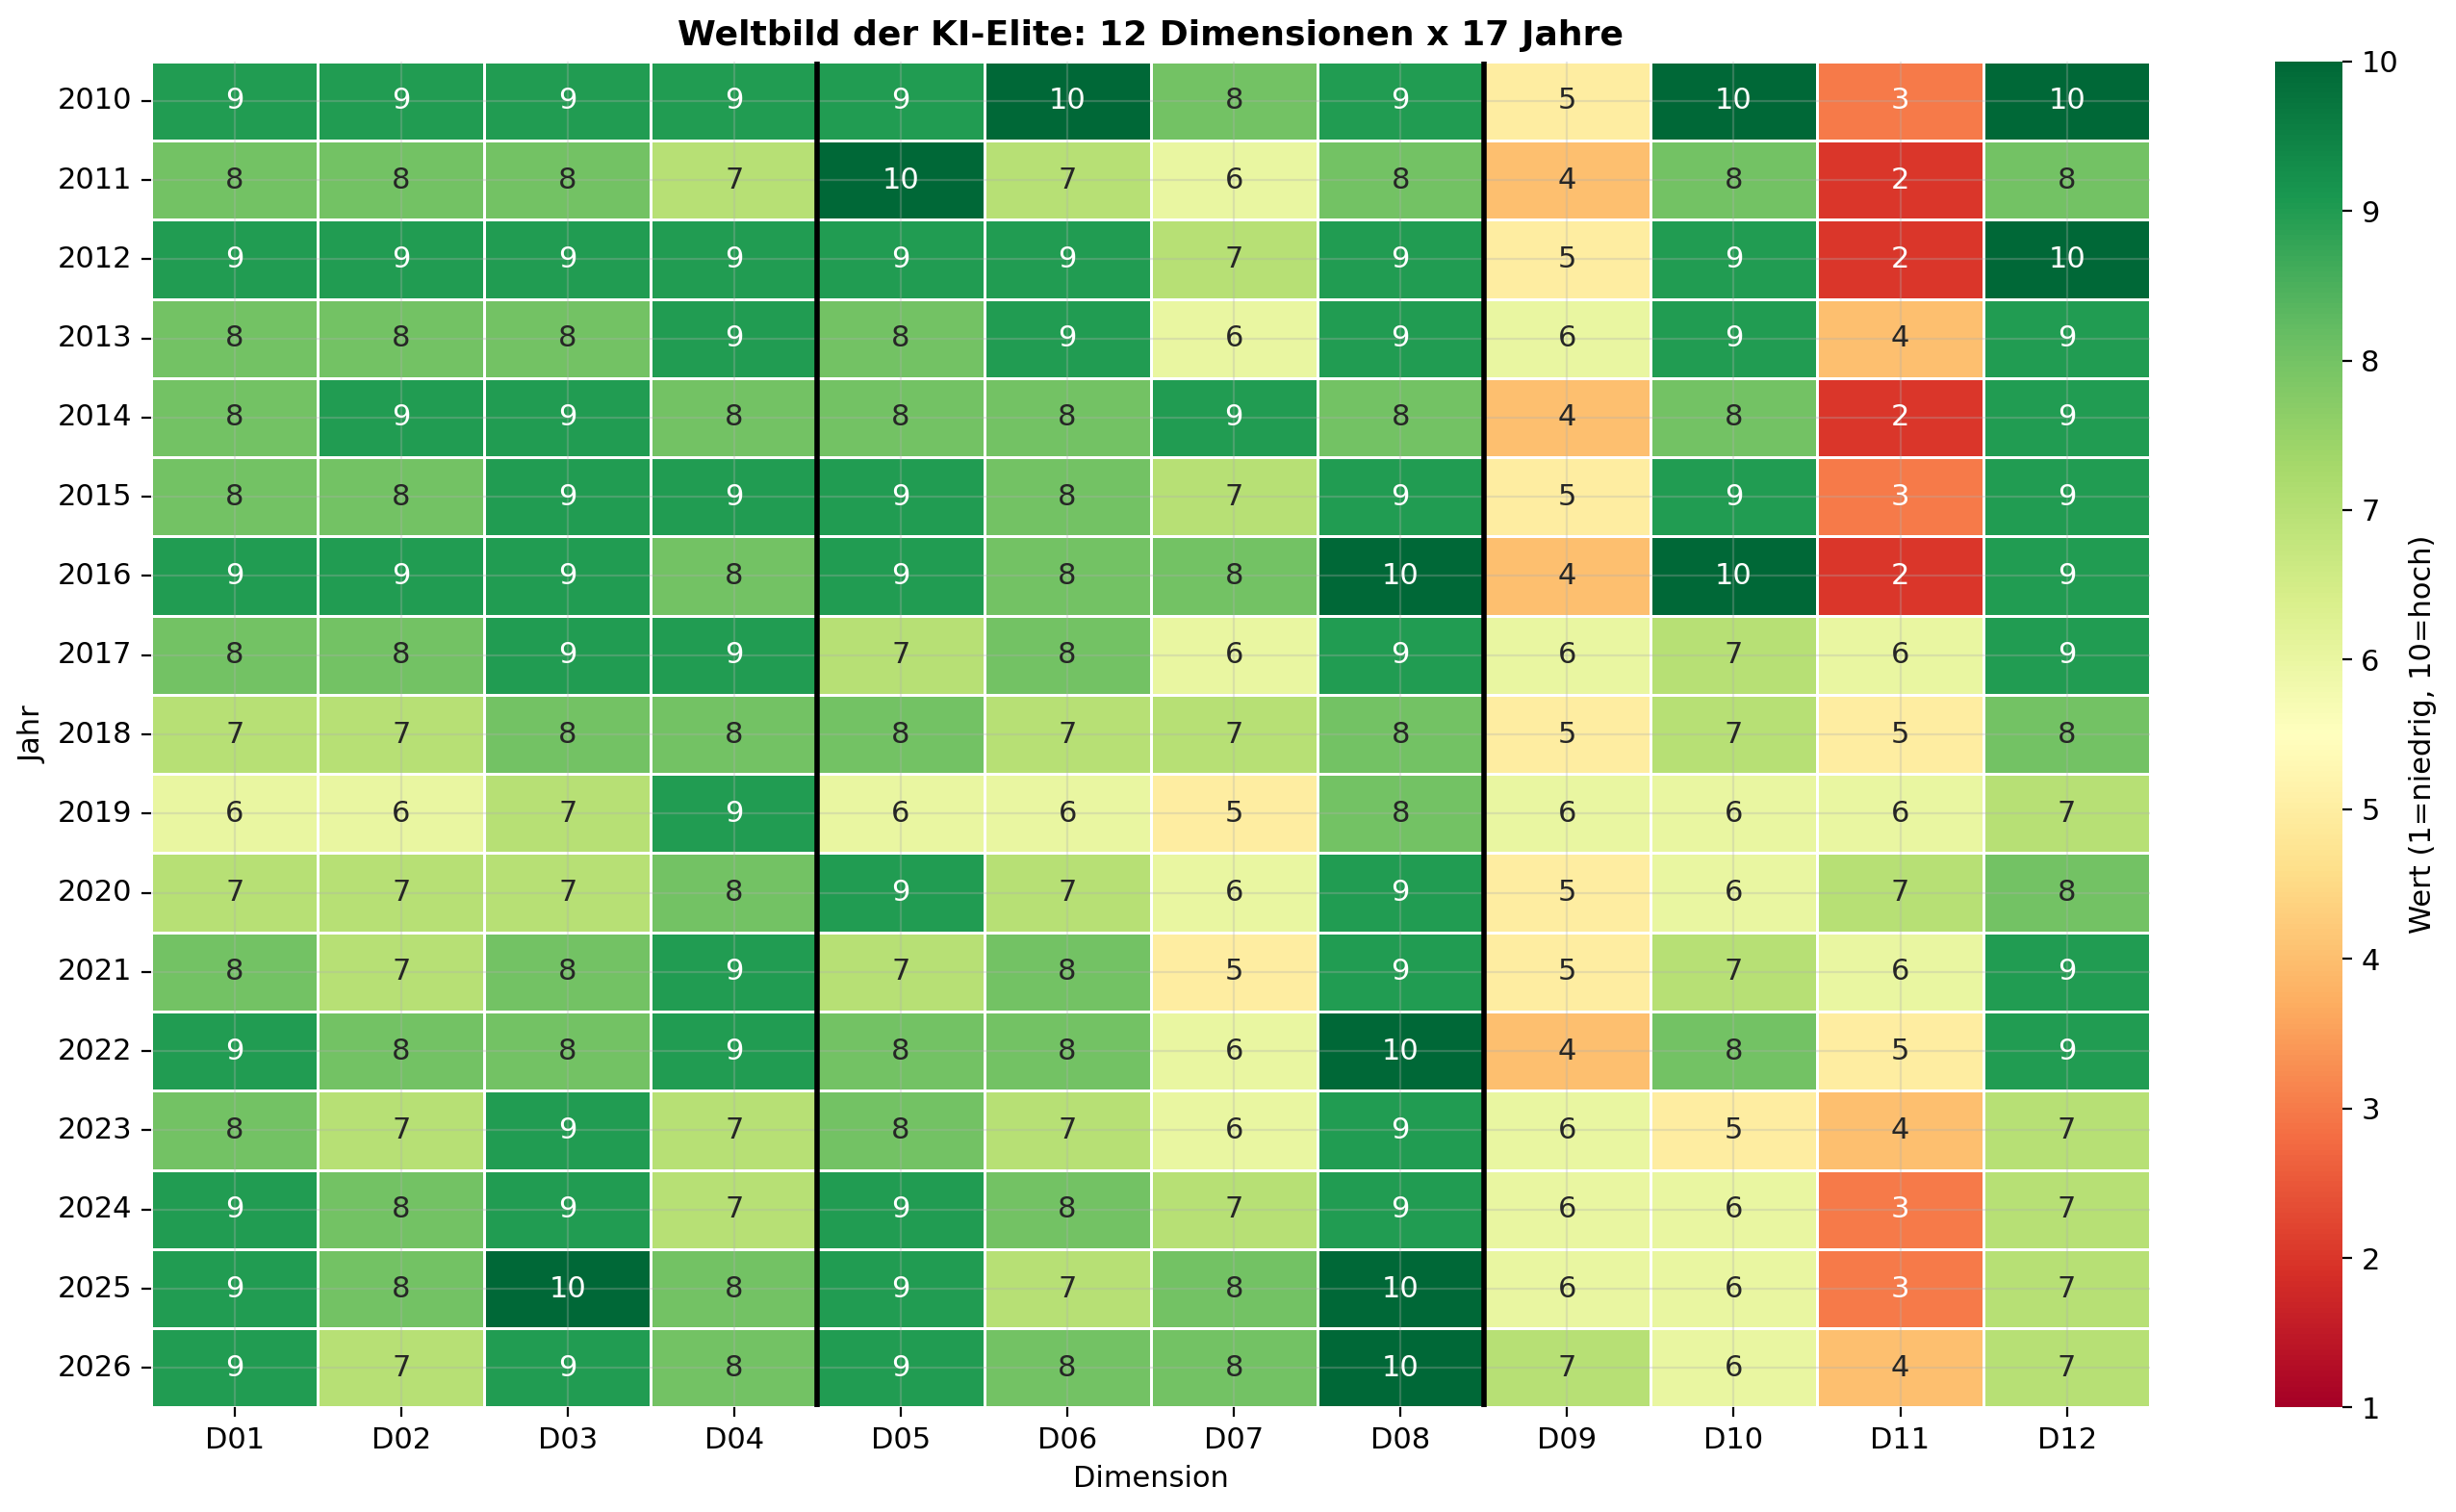
\includegraphics[width=0.95\textwidth]{fig2_heatmap.png}
  \caption{Heatmap der 12 Weltbild-Dimensionen \"uber alle untersuchten Gruppen. Hohe Werte (dunkel) markieren intensive \"Uberzeugungen; die Doppelsenke bei D09 und D11 ist \"uber alle Gruppen hinweg sichtbar.}
  \label{fig:heatmap}
\end{figure}


\subsubsection{Das Weltbild der Top~10}

Die zehn m\"achtigsten KI-Akteure vertreten dasselbe Weltbild in intensivierter Form (Avg~7,7). Auf zehn von zw\"olf Dimensionen liegen die Top-10-Werte exakt einen Skalenpunkt \"uber dem Kollektiv. Die beiden Ausnahmen: Menschenfreundlichkeit (D09=4) und Egalitarismus (D11=4) liegen \emph{niedriger}. Je m\"achtiger die Position, desto ausgepr\"agter das Sendungsbewusstsein und desto distanzierter das Menschenbild.


\subsubsection{Kern\"uberzeugungen}

Die Destillation der am h\"aufigsten wiederholten Aussagen (SE~5: HOM\_haeuf\_A, vgl.\ Anhang~\ref{app:se}) identifiziert f\"unf \"Uberzeugungen als Minimalkonsens: (1)~Technologie als moralisches Gebot, (2)~Elite-Steuerung, (3)~das Befreiungsnarrativ, (4)~geopolitischer Manich\"aismus, (5)~Arbeit als Identit\"at. Sicherheitsrhetorik geh\"ort zum Kernbestand des Diskurses, fungiert aber als diskursive Ressource, nicht als handlungsleitende \"Uberzeugung.

\medskip
\noindent\textbf{Kernbefund F1:} Die rekonstruierten Profile deuten auf ein koh\"arentes, hochintensives \"Uberzeugungssystem hin, das sich als \emph{technologischer Messianismus mit Ambivalenzstruktur} charakterisieren l\"asst. Die Bezeichnung \glqq Messianismus\grqq{} ist dabei als idealtypische Zuspitzung zu verstehen, nicht als psychologische Diagnose: Sie bezeichnet die spezifische \emph{Kombination} aus hohem Sendungsbewusstsein (D01), Techno-Determinismus (D05), Dringlichkeit (D08) und geringer anthropologischer Wertsch\"atzung (D09) -- ein Profil, das \"uber blo\ss{}es Sendungsbewusstsein hinausgeht, weil es technologischen Fortschritt als quasi-erl\"oserische Notwendigkeit rahmt.


\subsection{F2 -- Wandel des Weltbilds (l\"angsschnittlich)}
\label{sec:ergebnisse:f2}

\subsubsection{Entwicklung der 12 Dimensionen \"uber die Zeit}

Von zw\"olf Dimensionen zeigen vier ausgepr\"agte lineare Trends (Tabelle~\ref{tab:trends}).\footnote{Die hier berichteten Trendlinien beschreiben \textit{Muster in rekonstruierten Daten}: Die Weltbild-Werte sind LLM-gest\"utzte Rekonstruktionen, keine unabh\"angigen Messungen. OLS-Steigungen und $R^2$ dienen der Beschreibung der Verlaufsmuster, nicht der inferenzstatistischen Hypothesenpr\"ufung. Eine externe Validierung (Expertenratings vs.\ SWR-Output) steht noch aus (vgl.\ Abschnitt Limitations).}

\begin{table}[htbp]
  \centering
  \caption{Ausgepr\"agte lineare Trends (OLS-Beschreibung, $n=17$ Jahrespunkte).}
  \label{tab:trends}
  \begin{tabular}{l l c c}
    \toprule
    \textbf{Dimension} & \textbf{Richtung} & \textbf{Steigung/Dekade} & $R^2$ \\
    \midrule
    D10 Posthumanismus       & fallend  & $-2{,}4$ & $0{,}63$ \\
    D12 Kontroll\"uberzeugung & fallend  & $-1{,}5$ & $0{,}54$ \\
    D02 Selbstwirksamkeit    & fallend  & $-1{,}0$ & $0{,}31$ \\
    D09 Menschenfreundlichkeit & steigend & $+0{,}9$ & $0{,}27$ \\
    \bottomrule
  \end{tabular}
\end{table}

Den st\"arksten R\"uckgang verzeichnet der Posthumanismus (D10): von 10 im Jahr 2010 auf 6 im Jahr 2025. Die hohe Spearman-Rangkorrelation mit D12 ($r_s = +0{,}85$)\footnote{Die hier und im Folgenden berichteten Korrelationen (Spearman-Rangkorrelationen, berechnet \"uber die 17~Jahreszeitpunkte) sind \emph{Zusammenh\"ange innerhalb der LLM-Rekonstruktion}, nicht zwischen unabh\"angig gemessenen Variablen. Spearman wird verwendet, da die 12~Weltbild-Dimensionen Ordinalskalen darstellen; Pearson w\"urde Intervallskalenniveau voraussetzen, das hier nicht gegeben ist. Die Korrelationen k\"onnten interne Koh\"arenz des Modells widerspiegeln statt empirischer Zusammenh\"ange in der Realit\"at (vgl.\ Abschnitt~\ref{sec:limitationen}).} weist auf ein zusammenh\"angendes Ph\"anomen: Posthumanismus und Kontroll\"uberzeugung erodieren synchron. Der einzige deutlich steigende Wert betrifft die Menschenfreundlichkeit (D09), wobei die negative Korrelation mit D10 ($r_s = -0{,}58$) eine kompensatorische Verkn\"upfung nahelegt. Der Gesamtdurchschnitt bleibt nahezu konstant (Fr\"uhphase 7,5, Sp\"atphase 7,3), was eine tektonische Verschiebung unter der Oberfl\"ache verbirgt.

\begin{figure}[htbp]
  \centering
  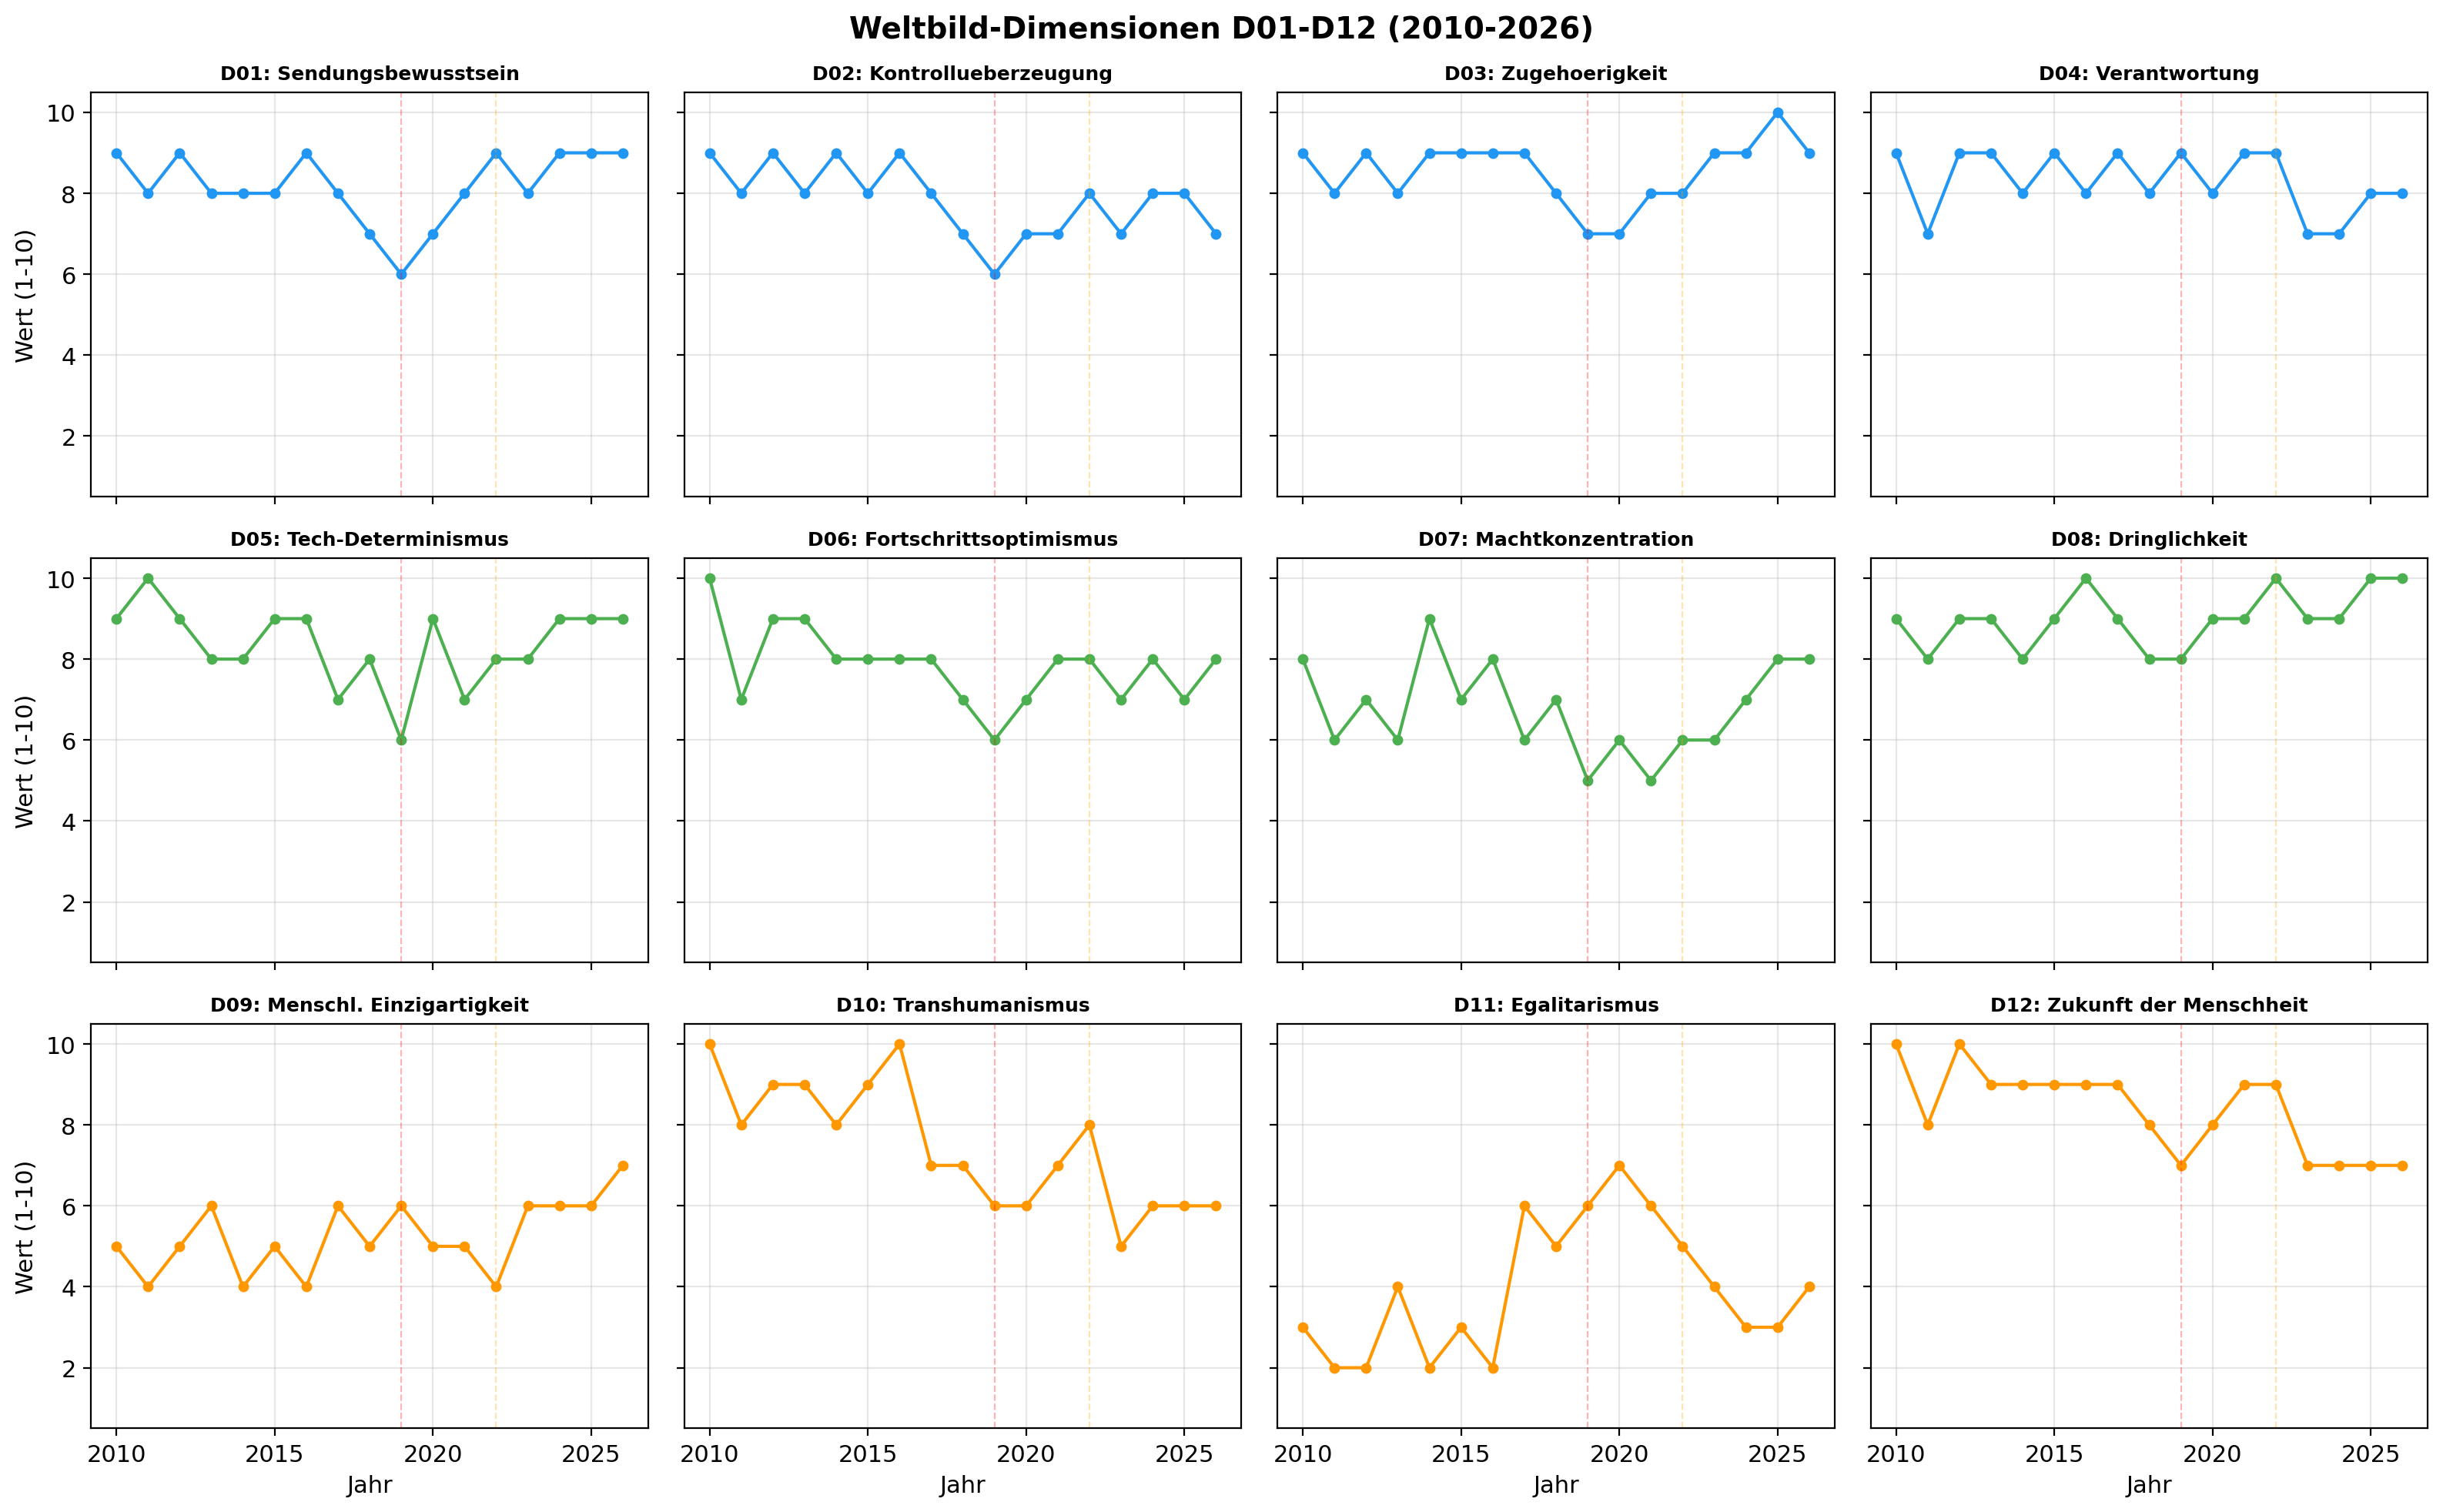
\includegraphics[width=\textwidth]{fig1_zeitreihen_panel.png}
  \caption{Zeitreihen der 12 Weltbild-Dimensionen (2010--2026). Ausgepr\"agte Trends sind hervorgehoben. Der markante Abfall von D10 (Posthumanismus) und D12 (Kontroll\"uberzeugung) bildet den \glqq Utopie-Komplex\grqq, dessen Zerfall durch steigende Dringlichkeit (D08) arithmetisch kompensiert wird.}
  \label{fig:zeitreihen}
\end{figure}

\begin{figure}[htbp]
  \centering
  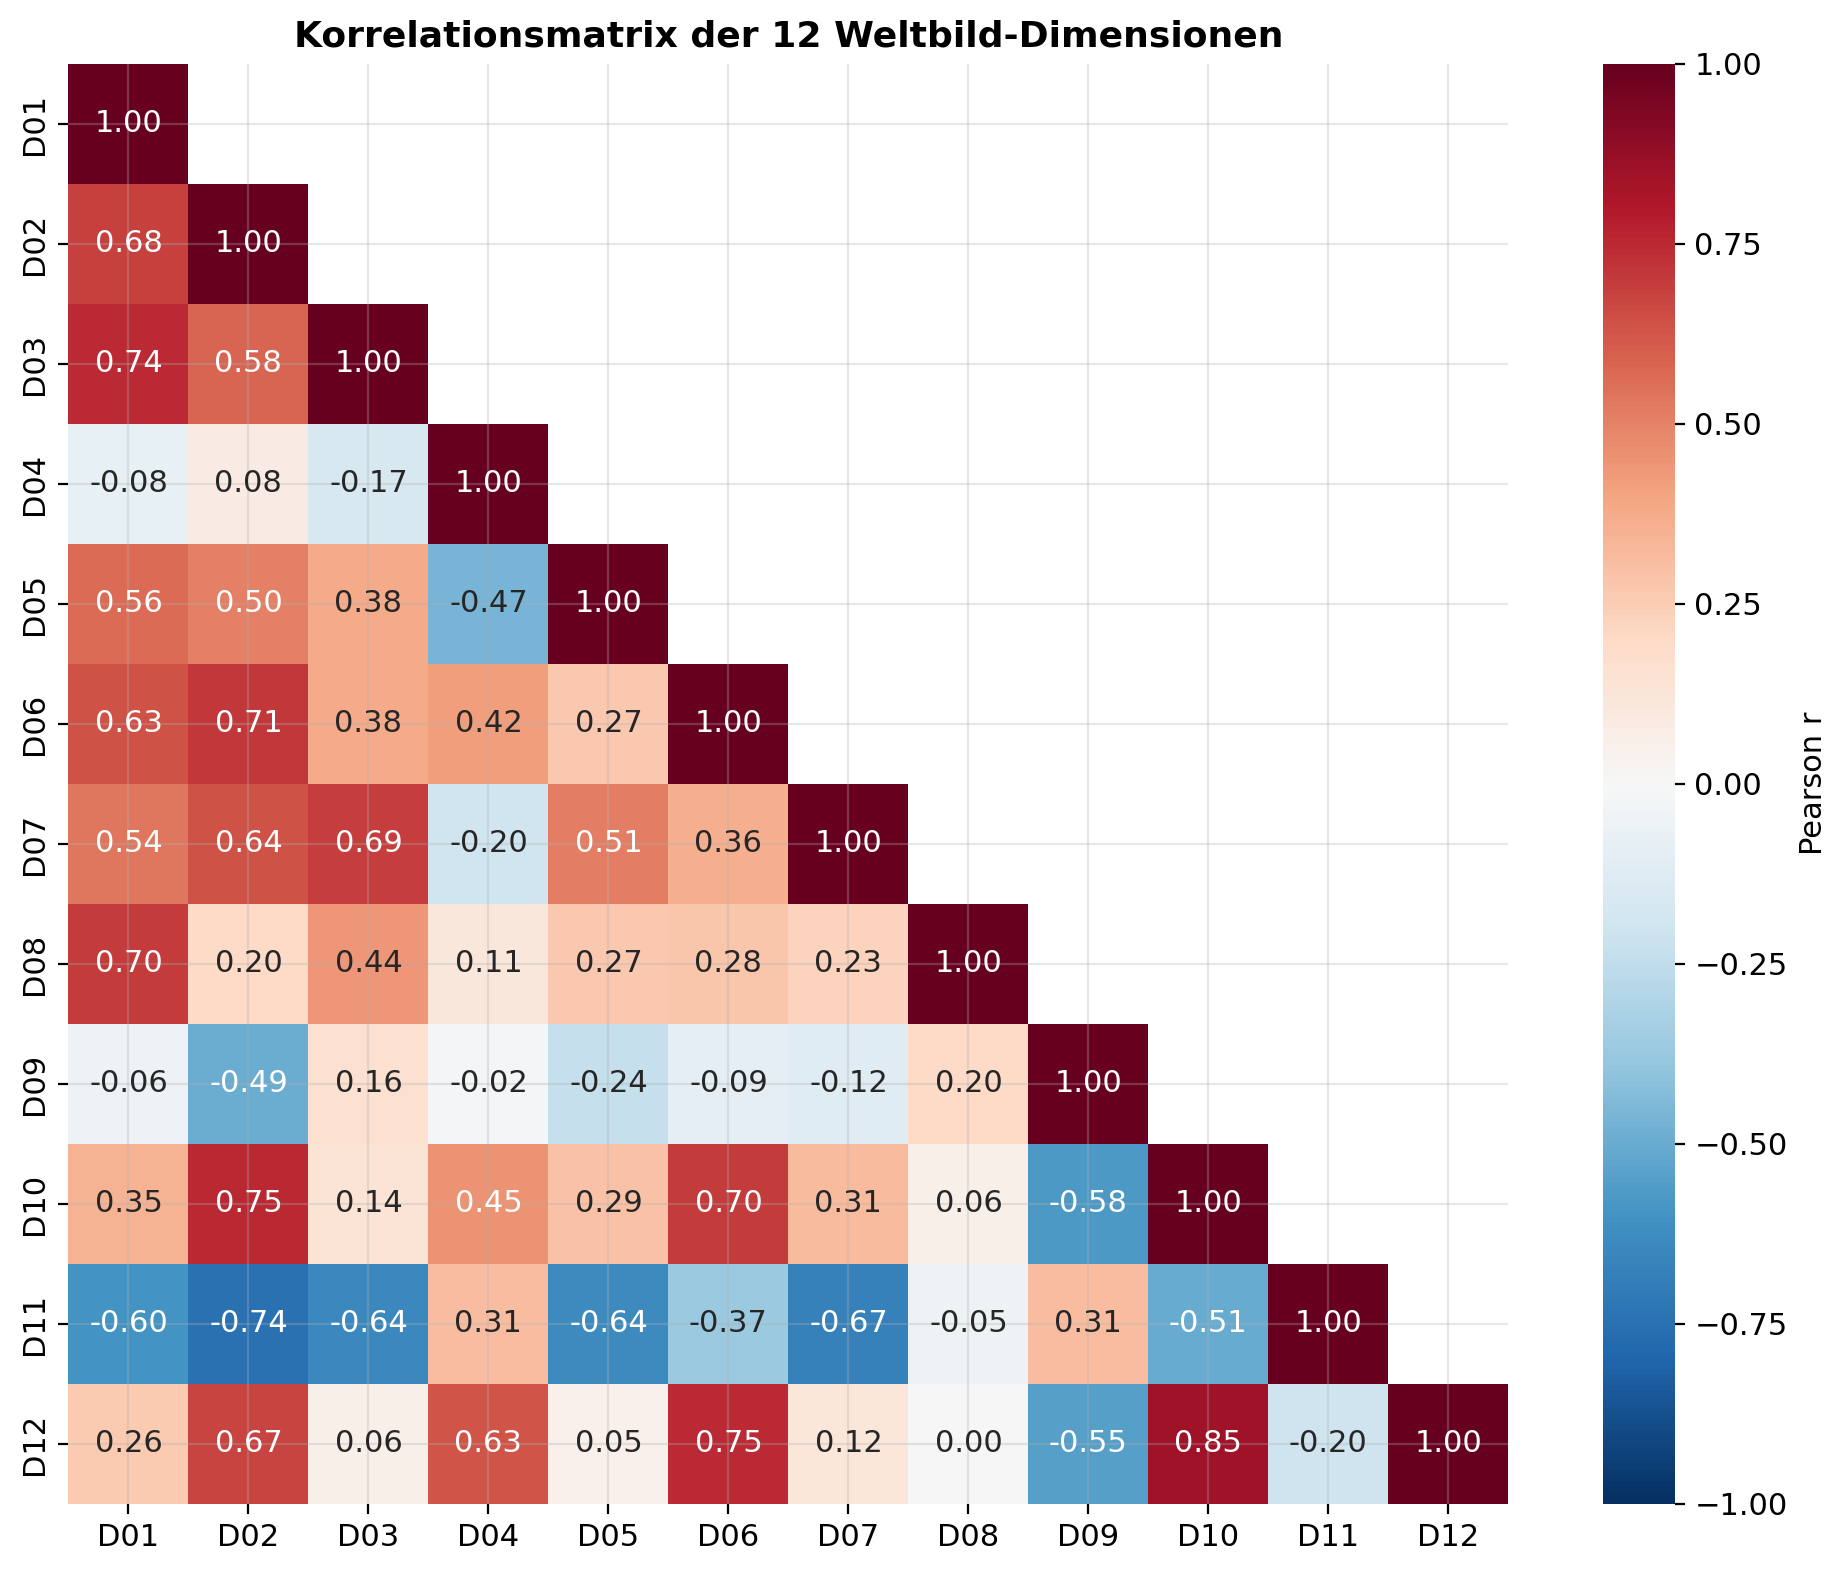
\includegraphics[width=0.85\textwidth]{fig4_korrelationsmatrix.png}
  \caption{Spearman-Rangkorrelationsmatrix der 12 Dimensionen. Die starke positive Korrelation zwischen D10 und D12 sowie die negative Korrelation zwischen D10 und D09 bilden den empirischen Kern des \glqq Utopie-Komplexes\grqq.}
  \label{fig:korrelationsmatrix}
\end{figure}


\subsubsection{Wendepunkte und Epochenvergleich}

Die Breakpoint-Detection -- durchgef\"uhrt als visuelle Inspektion der Zeitreihen, erg\"anzt durch die Identifikation synchroner Extrempunkte \"uber mehrere Dimensionen -- identifiziert zwei zentrale Wendepunkte.\footnote{Eine formale Breakpoint-Analyse (z.\,B.\ Bai-Perron-Test) war aufgrund der geringen Zahl von Zeitpunkten ($n=17$) und der Natur der Daten (LLM-Rekonstruktionen, keine unabh\"angigen Messungen) nicht sinnvoll anwendbar. Die Wendepunkte sind daher als \emph{deskriptive Beobachtungen} zu verstehen, nicht als statistisch gesicherte Strukturbr\"uche.} Der erste liegt bei 2019: Vier Dimensionen (D01, D02, D05, D06) erreichen synchron ihren Tiefpunkt, zeitlich assoziiert mit der GPT-2-Zur\"uckhaltung. Der zweite, dauerhaftere Wendepunkt liegt bei 2022/2023: Zeitgleich mit der ChatGPT-Ver\"offentlichung zeigt sich ein markanter Musterwechsel -- Dringlichkeit erreicht ihr rekonstruiertes Maximum (D08=10), Egalitarismus f\"allt von 6 auf 4. Im Unterschied zu 2019 kehren die Werte nicht zur\"uck; die rekonstruierten Profile nach 2022 deuten auf ein neues Gleichgewicht hin. Dabei ist zu beachten, dass die identifizierten Wendepunkte nicht isoliert von breiteren gesellschaftlichen Entwicklungen zu sehen sind: Die COVID-19-Pandemie (2020--2022) hat die Digitalisierungsdynamik beschleunigt und d\"urfte das Dringlichkeitserleben verst\"arkt haben; die zunehmende geopolitische Polarisierung (US-China-Technologiekonflikt) hat den \glqq manich\"aischen\grqq{} Aspekt des Weltbilds m\"oglicherweise befeuert; und der Beginn regulatorischer Initiativen (EU~AI~Act, 2021ff.) hat die Debatte um Governance versch\"arft. Diese Kontextfaktoren lassen sich mit der vorliegenden Methode nicht vom KI-spezifischen Wandel trennen.

\begin{figure}[htbp]
  \centering
  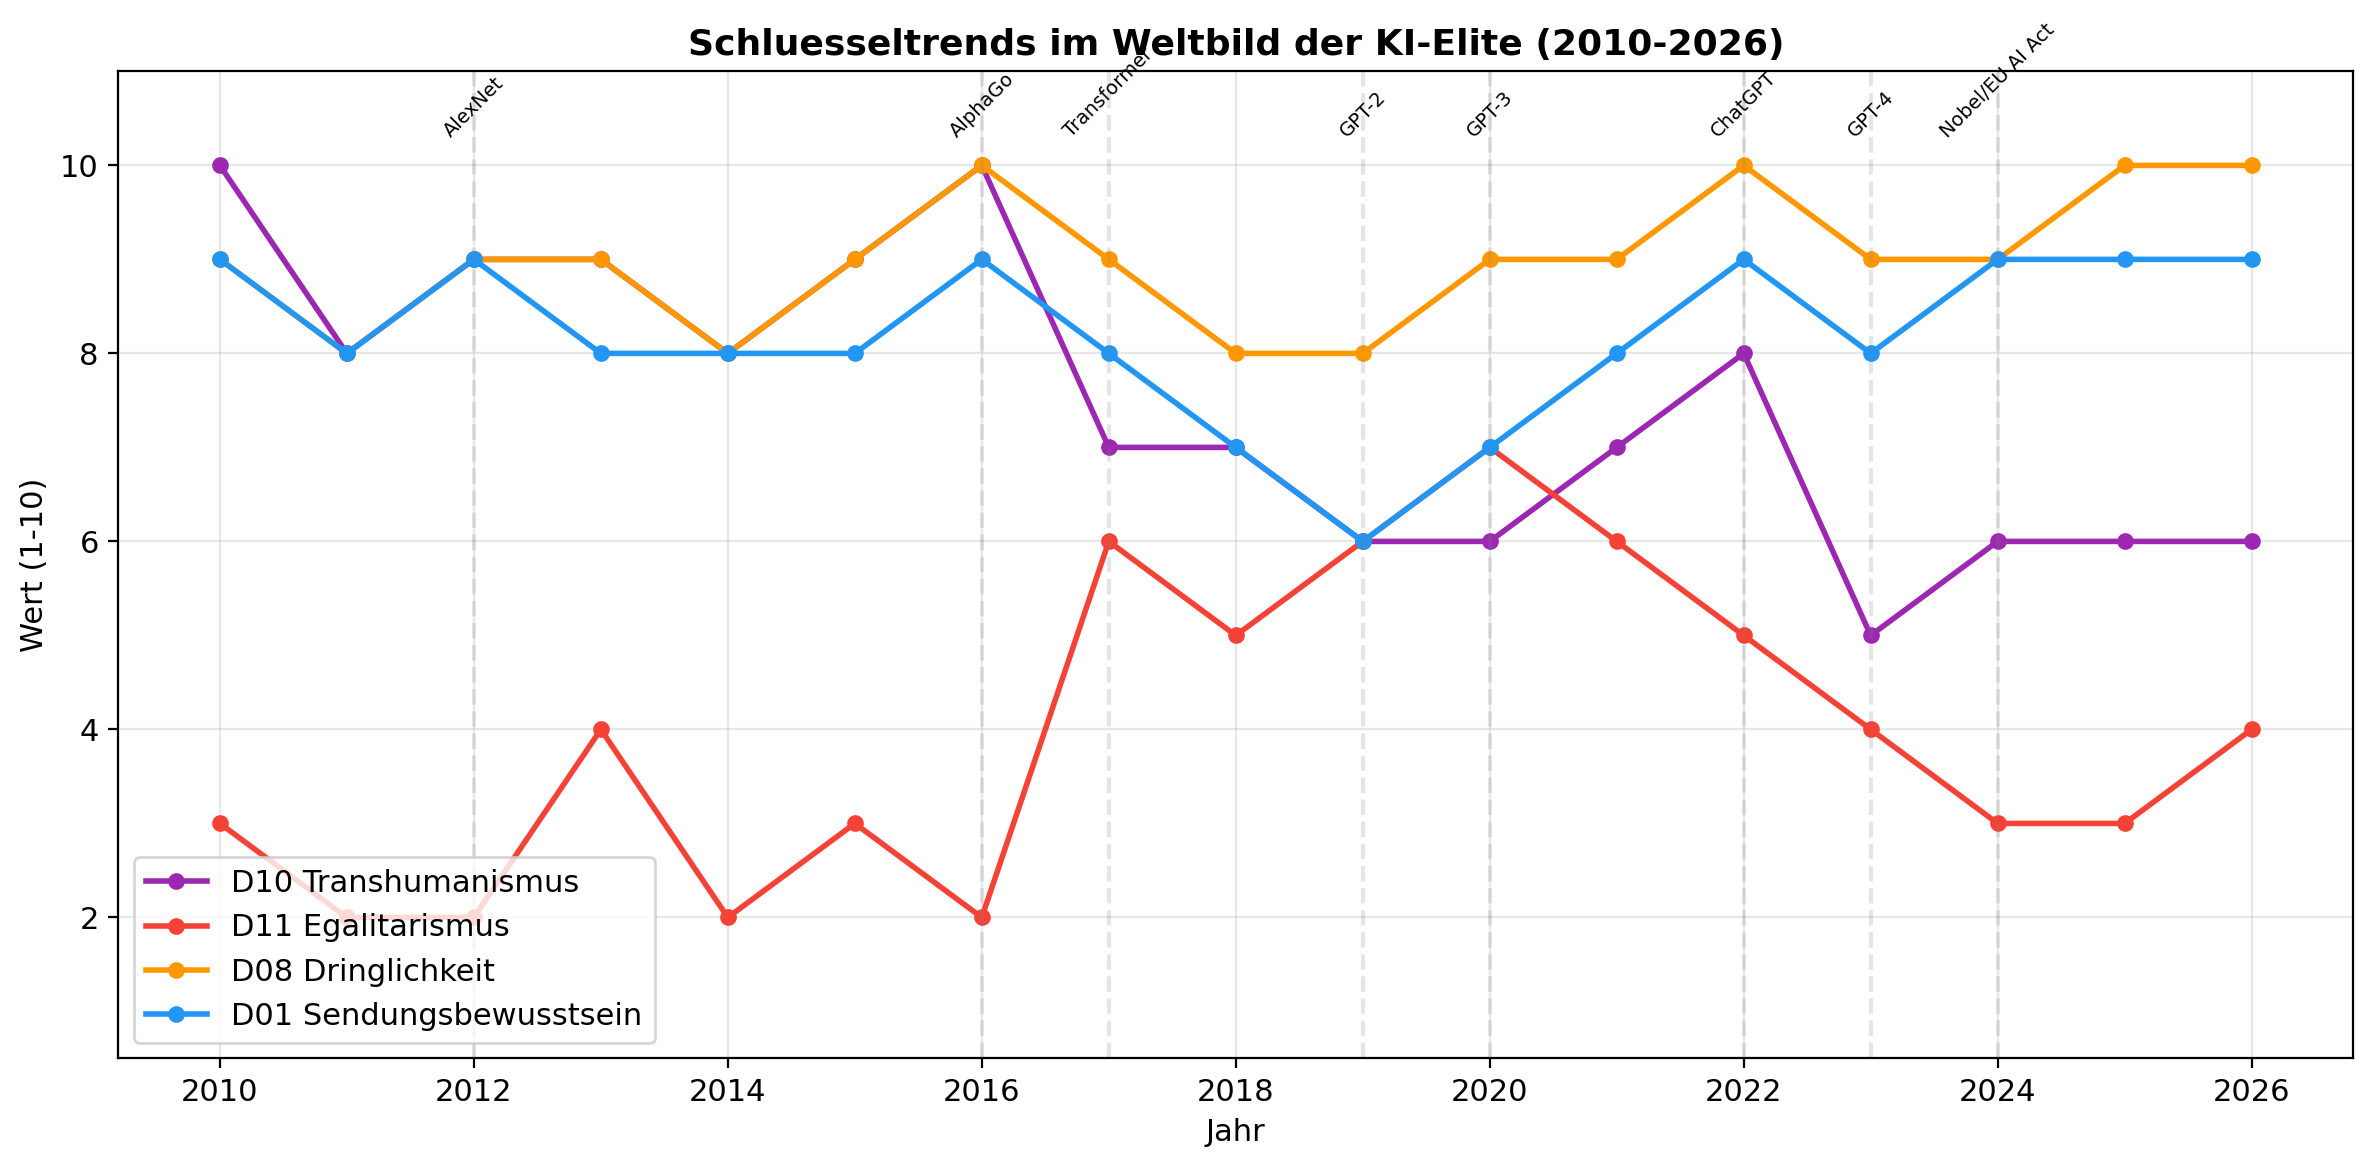
\includegraphics[width=0.95\textwidth]{fig7_schluesseltrends.png}
  \caption{Schl\"usseltrends der Weltbild-Transformation. Die zwei Wendepunkte (2019, 2022/2023) und die drei Epochen (Prometheischer Optimismus, Erste Ambivalenz, Tragisches Bewusstsein) sind markiert.}
  \label{fig:schluesseltrends}
\end{figure}


\subsubsection{Konvergenz oder Divergenz?}

Die Daten zeigen eine zunehmende Ausdifferenzierung. Der ChatGPT-Effekt intensiviert sowohl die Architekten-Position (Beschleunigung, Machtkonzentration) als auch die H\"uter-Position (Vorsicht, Regulierung) gleichzeitig -- er wirkt als Katalysator der Bipolarisierung.


\subsubsection{Metaphern- und Emotions-Wandel}

Die Leitmetapher verschiebt sich von Prometheus -- dem Feuerbringer -- zum tragischen Helden, der retten muss, was m\"oglicherweise nicht mehr zu retten ist. Die Handlung bleibt dieselbe (Beschleunigung), aber ihre emotionale Rahmung dreht sich um: nicht mehr aus Euphorie, sondern aus dem Glauben, dass die Alternative schlimmer w\"are.

\medskip
\noindent\textbf{Kernbefund F2:} Die rekonstruierten Profile deuten auf eine strukturelle Transformation des Weltbilds hin -- von einer monochromen Utopie zu einer bimodalen Wette. \emph{Tragisch} im Sinne der Bezeichnung \glqq tragischer Beschleunigungszwang\grqq{} meint die gleichzeitige Erosion utopischer Gewissheiten und Persistenz der Handlungsrichtung: Die Akteure beschleunigen, obwohl sie an der Zukunft zweifeln, die sie bauen -- weil sie die Alternativen (geopolitischer R\"uckfall, Kontrollverlust an weniger verantwortungsvolle Akteure) als schlimmer bewerten. Drei Erosionstrends (D10, D12, D02) bilden einen \glqq Utopie-Komplex\grqq, dessen Zerfall durch steigende Dringlichkeit (D08) arithmetisch kompensiert wird. Allerdings ist nicht auszuschlie\ss{}en, dass der R\"uckgang des Posthumanismus (D10) teilweise ein Artefakt ver\"anderter \"offentlicher Diskurse ist: Wenn das Thema medial weniger pr\"asent ist, sinkt auch die Datendichte entsprechender Aussagen, was die LLM-Rekonstruktion verzerren kann.


\subsection{F3 -- Kongruenz von Aussagen und Handlungen}
\label{sec:ergebnisse:f3}

\begin{table}[htbp]
  \centering
  \caption{Vergleich Aussagen (A) und Handlungen (H), $N=100$. Werte sind Einzel-Run-Ratings auf Gruppenebene (v2, mit strikter Instanztrennung). v1-Werte (Same-Instance-Ratings) zum Vergleich.}
  \label{tab:kongruenz}
  \begin{tabular}{l c c c c c}
    \toprule
    \textbf{Dimension} & \textbf{Sagen v2} & \textbf{Handeln v2} & $\Delta$\textbf{v2} & $\Delta$\textbf{v1} & \textbf{Stabil?} \\
    \midrule
    D01 Sendungsbewusstsein     & 9 & 9 & $0$  & $-1$ & -- \\
    D02 Selbstwirksamkeit       & 8 & 9 & $+1$ & $+1$ & \checkmark \\
    D03 Arbeitsethos            & 9 & 9 & $0$  & $+1$ & -- \\
    D04 Verantwortungsgef\"uhl  & 8 & 8 & $0$  & $-2$ & -- \\
    D05 Techno-Determinismus    & 7 & 9 & $\mathbf{+2}$ & $+1$ & $\uparrow$ \\
    D06 Fortschrittsglaube      & 8 & 8 & $0$  & $-1$ & -- \\
    D07 Machtkonzentration      & 6 & 8 & $\mathbf{+2}$ & $+2$ & \checkmark\checkmark \\
    D08 Dringlichkeit           & 9 & 9 & $0$  & $+1$ & -- \\
    D09 Menschenfreundlichkeit  & 6 & 5 & $-1$ & $-2$ & $\downarrow$ \\
    D10 Posthumanismus          & 7 & 7 & $0$  & $+1$ & -- \\
    D11 Egalitarismus           & 5 & 3 & $\mathbf{-2}$ & $-3$ & \checkmark\checkmark \\
    D12 Kontroll\"uberzeugung   & 7 & 8 & $+1$ & $-1$ & -- \\
    \midrule
    \textbf{Durchschnitt}       & \textbf{7,4} & \textbf{7,7} & $+0{,}3$ & $-0{,}4$ & \\
    MAE                         &   &   & $0{,}75$ & $1{,}42$ & \\
    \bottomrule
  \end{tabular}
\end{table}

\noindent\textbf{Methodische Anmerkung:} Die v1-Ratings (in fr\"uheren Versionen dieser Studie berichtet) wurden innerhalb derselben LLM-Instanz generiert, wodurch Kreuzkontamination zwischen Aussagen- und Handlungsprofilen m\"oglich war. Die hier gezeigten v2-Ratings verwenden strikte Instanztrennung: Jeder Datentyp wurde von einem unabh\"angigen Agenten ohne Zugang zum anderen verarbeitet. Dies reduzierte die Gesamtkluft von MAE $= 1{,}42$ auf MAE $= 0{,}75$ ($-47\,\%$), und die v2-Kluft f\"allt unter die Kontrollbaseline (G6~v2: MAE $= 0{,}92$). Das bedeutet: Die \emph{Gesamt}-Sagen-Handeln-Kluft ist in Einzeldurchl\"aufen nicht zuverl\"assig vom Messrauschen unterscheidbar.

Allerdings zeigen zwei spezifische Dimensionen \emph{stabile} Diskrepanzen \"uber beide Messbedingungen: \textbf{D07 Machtkonzentration} ($\Delta = +2$ in v1 und v2) und \textbf{D11 Egalitarismus} ($\Delta = -2$ in v2, $-3$ in v1). Diese bilden die robusten Sagen-Handeln-Befunde der Studie. Handlungen konzentrieren Macht st\"arker als die Rhetorik nahelegt, und Handlungen sind weniger egalit\"ar als die Rhetorik behauptet. Beides ist konsistent mit einer strukturellen \emph{Erw\"unschtheits-Asymmetrie}: Der \"offentliche Diskurs \"ubersch\"atzt egalit\"are und demokratische Commitments relativ zum operativen Verhalten.

\begin{figure}[htbp]
  \centering
  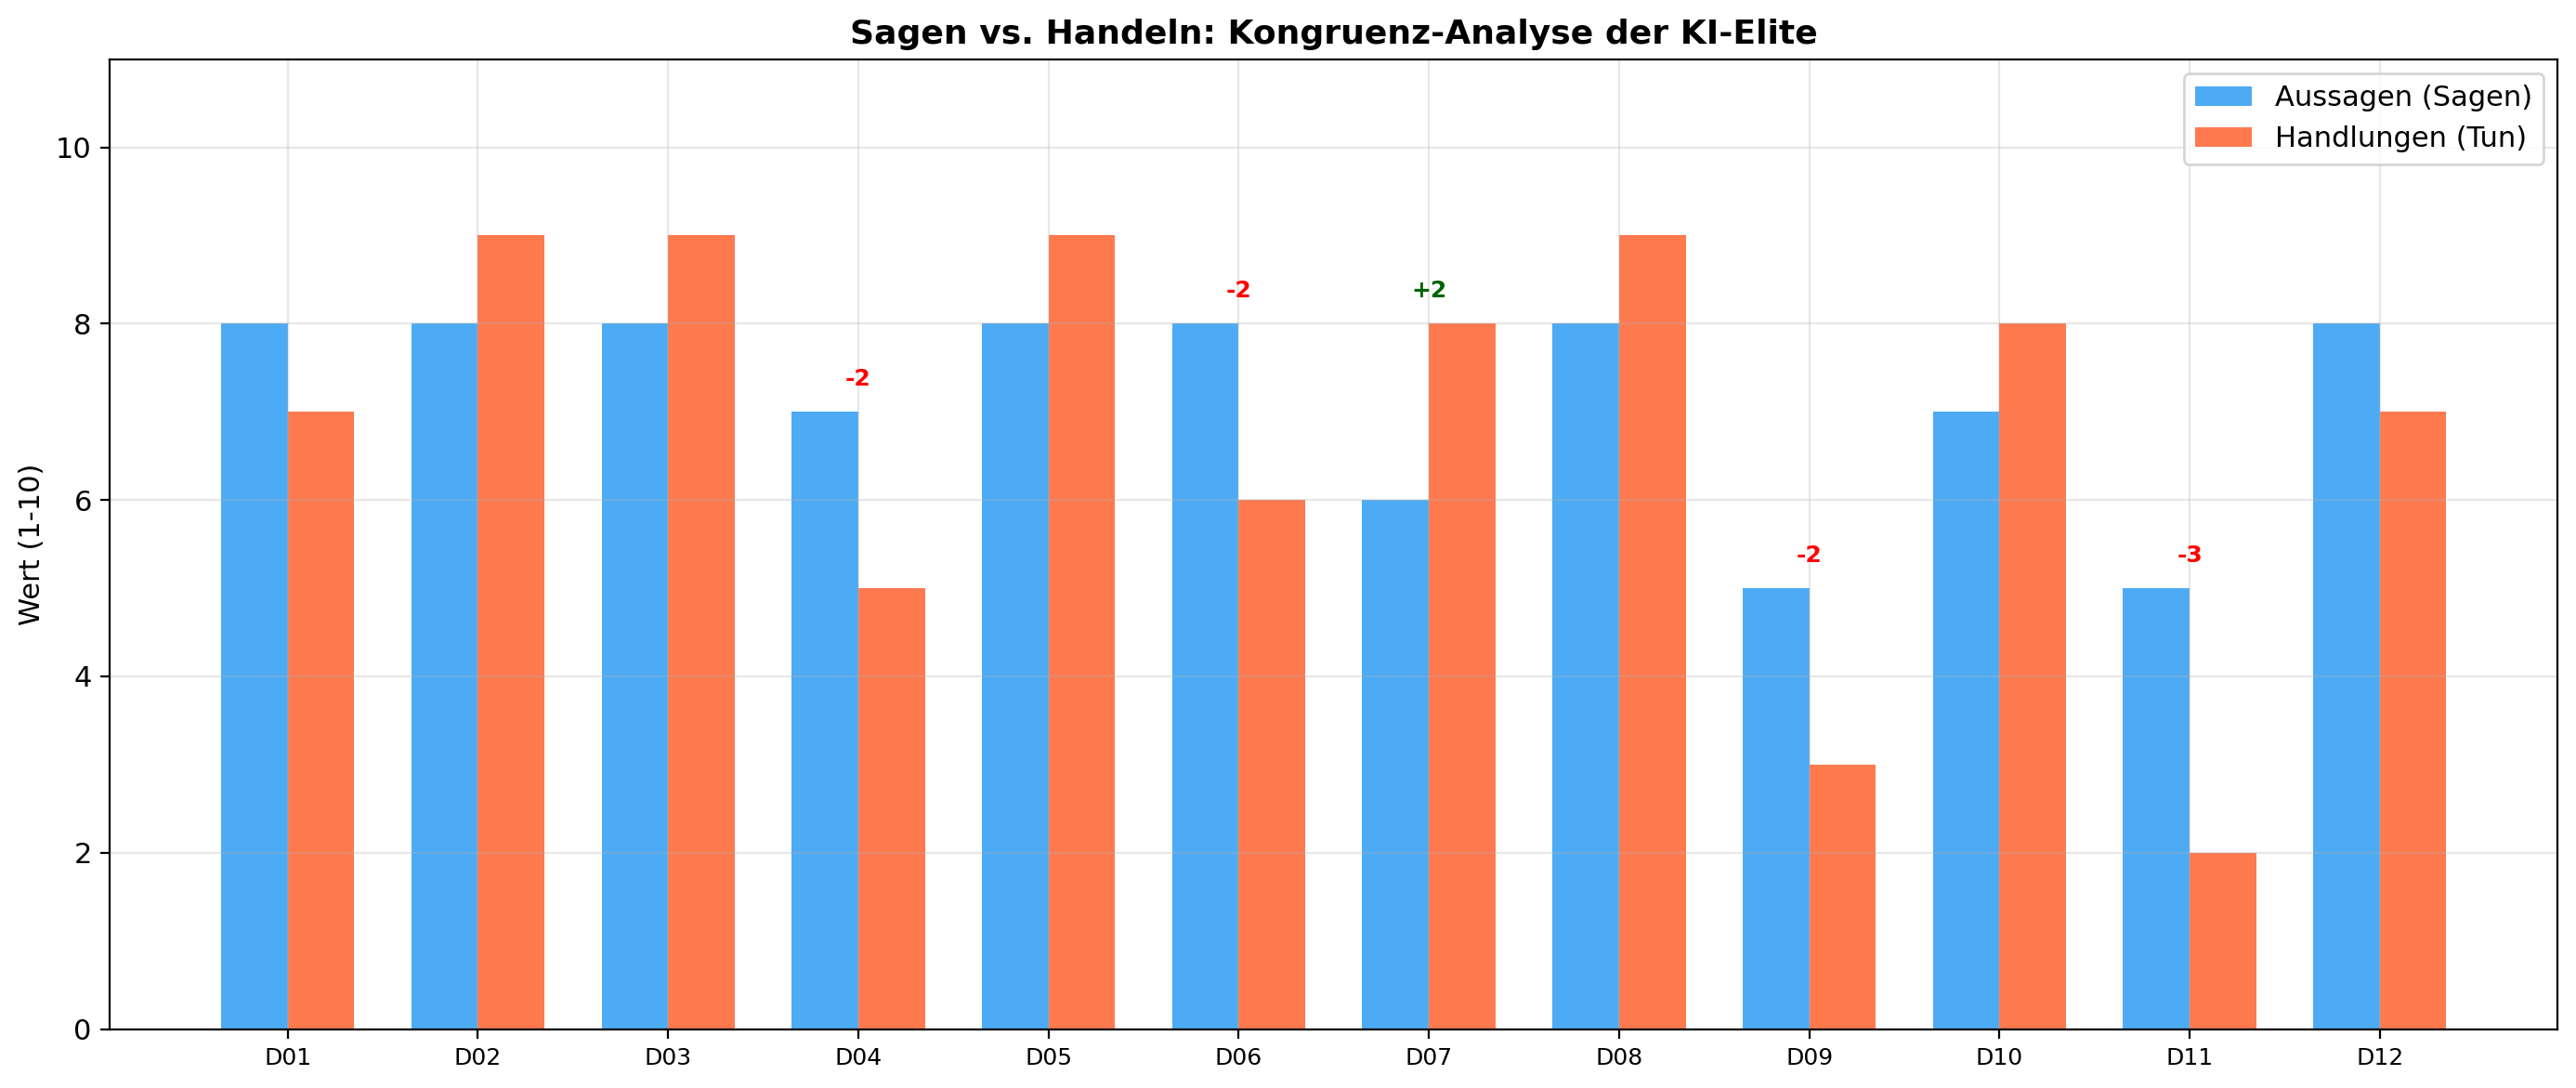
\includegraphics[width=0.95\textwidth]{fig6_sagen_vs_handeln.png}
  \caption{Sagen vs.\ Handeln: Vergleich der aus Aussagen (A) und Handlungen (H) rekonstruierten Weltbilder. Die gesellschaftsorientierten Dimensionen (D04, D06, D09, D11) fallen im Handeln systematisch ab, w\"ahrend die machtbezogenen Dimensionen (D07, D05) im Handeln steigen.}
  \label{fig:sagen_handeln}
\end{figure}

Die gr\"o\ss{}te stabile Einzeldiskrepanz (D11, $\Delta\,-2$ in v2, $-3$ in v1) zeigt: In Aussagen spricht die KI-Elite von \glqq Zugang f\"ur alle\grqq; in ihren Handlungen baut sie Mehrfach-Stimmrechtsaktien, konzentriert Compute-Infrastruktur und schafft exklusive Netzwerke. D07 (Machtkonzentration, $\Delta\,+2$) ist der komplement\"are Befund: Die Rhetorik favorisiert verteilte Governance, aber operative Entscheidungen zentralisieren Kontrolle.

\subsubsection{Gruppen-Dekomposition der Sagen-Handeln-Kluft}

Der aggregierte Sagen-Handeln-Vergleich verdeckt substanzielle gruppenspezifische Variation -- ein Simpson-Paradox. Wenn f\"unf soziologische Gruppen mit strikter Instanztrennung analysiert werden (Aussagen- und Handlungskorpus von unabh\"angigen Agenten verarbeitet), emergieren drei distinkte Muster:

\begin{itemize}
\item \textbf{CEOs} (MAE $= 1{,}08$, \"uber Baseline): Der klassische Erw\"unschtheits-Gap. Rhetorik ist egalit\"arer (D11: Sagen~5, Handeln~3, $\Delta = -2$) und weniger machtkonzentrierend (D07: Sagen~7, Handeln~9, $\Delta = +2$) als operatives Verhalten. CEOs sagen das \glqq Richtige\grqq{} \"uber verteilte Governance und bauen gleichzeitig Dual-Class-Aktienstrukturen.

\item \textbf{Risiko-Warner} (MAE $= 1{,}92$, st\"arkster Gap): Kein inverser Gap, sondern \emph{prophetische Konsistenz}. Bei Dekomposition nach abh\"angiger Variable wird das Muster klar: DV1 (Selbstbild, D01--D04) zeigt nahezu perfekte Konsistenz (MAE $= 0{,}8$) -- Risiko-Warner wissen, wer sie sind. Die Diskrepanz konzentriert sich in DV3 (Menschenbild, MAE $= 3{,}2$): Ihre \emph{Aussagen} beschreiben eine gef\"urchtete Zukunft -- Mensch als ersetzbar (D09: Sagen~4), posthumanistische Transformation als unvermeidlich (D10: Sagen~9) -- w\"ahrend ihre \emph{Handlungen} ihre tats\"achlichen Werte offenbaren: hohe Menschenfreundlichkeit (D09: Handeln~8), Ablehnung des Posthumanismus in der Praxis (D10: Handeln~4), aktive Handlungsf\"ahigkeit (D12: Handeln~8). Dies ist die Struktur prophetischer Warnung: eine M\"oglichkeitsprojektion artikulieren, die man \emph{verhindern} will, und dann konsequent dagegen handeln. Ihr Sagen-Handeln-Gap ist keine Heuchelei, sondern die Signatur antizipatorischer Ethik -- ein Befund, der ohne Gruppendekomposition unsichtbar bliebe.

\item \textbf{Investoren} (MAE $= 0{,}75$, unter Baseline): Die konsistenteste Gruppe. Rhetorik und Handeln erz\"ahlen dieselbe Geschichte: radikaler Techno-Optimismus mit minimaler egalit\"arer Orientierung. Kein Erw\"unschtheits-Gap -- sie meinen, was sie sagen.

\item \textbf{Beschleuniger} (MAE $= 0{,}92$, an Baseline): Ein Grenzmuster, das einer schw\"acheren Version des CEO-Gaps \"ahnelt. Rhetorik ist optimistischer hinsichtlich Fortschritt (D06: $\Delta = -2$), verantwortungsvoller (D04: $\Delta = -2$) und egalit\"arer (D11: $\Delta = -2$) als operatives Verhalten.
\end{itemize}

\noindent Diese entgegengesetzten gruppenspezifischen Gaps heben sich im Aggregat auf (Gesamt-MAE $= 0{,}75$, unter der G6-v2-Kontrollbaseline von $0{,}92$). Die Sagen-Handeln-Kluft ist nicht absent -- sie ist \emph{gruppenspezifisch und richtungsabh\"angig} und erfordert Dekomposition statt aggregierter Berichterstattung.

\medskip
\noindent\textbf{Kernbefund F3:} Zwei robuste Sagen-Handeln-Diskrepanzen \"uberstehen die Instanztrennung: D07~(Machtkonzentration) und D11~(Egalitarismus). Die Gesamtmagnitude der Kluft ist messbedingt variabel und sollte in Einzeldurchl\"aufen nicht \"uberinterpretiert werden. Aber die \emph{Richtung} der Asymmetrie ist stabil: Der \"offentliche Diskurs ist egalit\"arer und machtverteilender als das operative Verhalten. Eine formale Quantifizierung (mit Konfidenzintervallen aus $N \geq 30$ wiederholten Messungen) bleibt ein Desiderat.


\subsection{F4 -- Weltbild-Cluster}
\label{sec:ergebnisse:f4}

Aus den Daten lassen sich vier distinkte Weltbild-Typen identifizieren (Tabelle~\ref{tab:typen}).

\textbf{Identifikationsmethode:} Die Cluster-Identifikation erfolgte in einem zweistufigen Verfahren. \emph{Stufe~1 (LLM-gest\"utzt):} Alle 15 Gruppen-Synthesen wurden nach \"Ahnlichkeitsmustern in den 12~Dimensionen gruppiert, wobei die gr\"o\ss{}ten Varianzachsen (D07~Machtkonzentration, D09~Menschenfreundlichkeit, D11~Egalitarismus) als Trennmerkmale fungierten. \emph{Stufe~2 (Autor-Validierung):} Die vom LLM vorgeschlagene Vier-Cluster-L\"osung wurde vom Autor anhand inhaltlicher Koh\"arenz und Plausibilit\"at evaluiert. Alternative L\"osungen (drei und f\"unf Cluster) wurden gepr\"uft und verworfen: Drei Cluster verschmelzen Innovator und Befreier, was inhaltlich nicht gerechtfertigt ist; f\"unf Cluster spalten den H\"uter-Typ in eine Untergruppe, die empirisch nicht stabil reproduziert werden konnte. Wir betonen, dass diese Cluster-Identifikation \emph{explorativ} ist -- eine konfirmatorische Validierung an einem unabh\"angigen Datensatz steht aus. Die Cluster-L\"osung ist eine \emph{interpretative Hypothese}, nicht ein statistisch abgesichertes Ergebnis im Sinne formaler Clusteranalyse.

\begin{table}[htbp]
  \centering
  \caption{Die vier Weltbild-Typen der KI-Elite. Die Werte sind Cluster-Durchschnitte aus den Gruppen-Synthesen; individuelle Abweichungen innerhalb eines Clusters k\"onnen erheblich sein (vgl.\ die Andreessen-Diskrepanz in der nachfolgenden Fu\ss{}note).}
  \label{tab:typen}
  \small
  \begin{tabular}{l c c c c}
    \toprule
    \textbf{Merkmal} & \textbf{I \glqq Architekt\grqq} & \textbf{II \glqq H\"uter\grqq} & \textbf{III \glqq Innovator\grqq} & \textbf{IV \glqq Befreier\grqq} \\
    \midrule
    $n$ & 35 & 25 & 22 & 18 \\
    Prototyp & CEOs, Investoren & Akademiker, Risiko-W. & Gr\"under & Open Source \\
    Avg D01--D12 & 7,8 & 6,4 & 7,2 & 6,8 \\
    D04 Verantwortung & 6,3 & \textbf{9,0} & 8,3 & 6,0 \\
    D07 Machtkonzentr. & \textbf{8,8} & 4,8 & 6,5 & \textbf{2,5} \\
    D09 Menschenfreundl. & \textbf{3,3} & 5,8 & 4,8 & \textbf{6,5} \\
    D11 Egalitarismus & \textbf{2,8} & \textbf{7,2} & 5,0 & \textbf{7,5} \\
    \bottomrule
  \end{tabular}
\end{table}

Der \textbf{Architekt} vereint maximales Sendungsbewusstsein mit minimalem Egalitarismus: Machtkonzentration ist Voraussetzung f\"ur Handlungsf\"ahigkeit. Der \textbf{H\"uter} bildet den Gegenpol: maximale Verantwortung, Forderung nach institutioneller Begrenzung. Der \textbf{Innovator} steht dazwischen. Der \textbf{Befreier} ist die \"uberraschendste Entdeckung: minimale Machtkonzentration \emph{und} hoher Egalitarismus -- Regulierungsgegner, die Macht radikaler verteilen wollen als alle anderen, allerdings durch M\"arkte und Open-Source-Communities.\footnote{Der hohe D11-Wert des Befreier-Typs (7,5) und der niedrige D11-Wert einzelner Prototypen (z.\,B.\ Andreessen: D11=2) markieren eine Konstruktvalidit\"atsproblem: D11 misst Gleichheitsorientierung, nicht deren \emph{Mechanismus}. Marktlibertaerer Zugangs-Egalitarismus (Befreier) und redistributiver Egalitarismus (H\"uter) produzieren \"ahnliche Skalenwerte auf D11, meinen aber Verschiedenes. Der Prototyp-Wert bezieht sich auf die Einzelperson-Synthese, der Cluster-Wert auf das Gruppenaggregat -- Andreessens individuelles Profil weicht vom Cluster-Durchschnitt ab. K\"unftige Operationalisierungen sollten hier differenzieren.}

\begin{figure}[htbp]
  \centering
  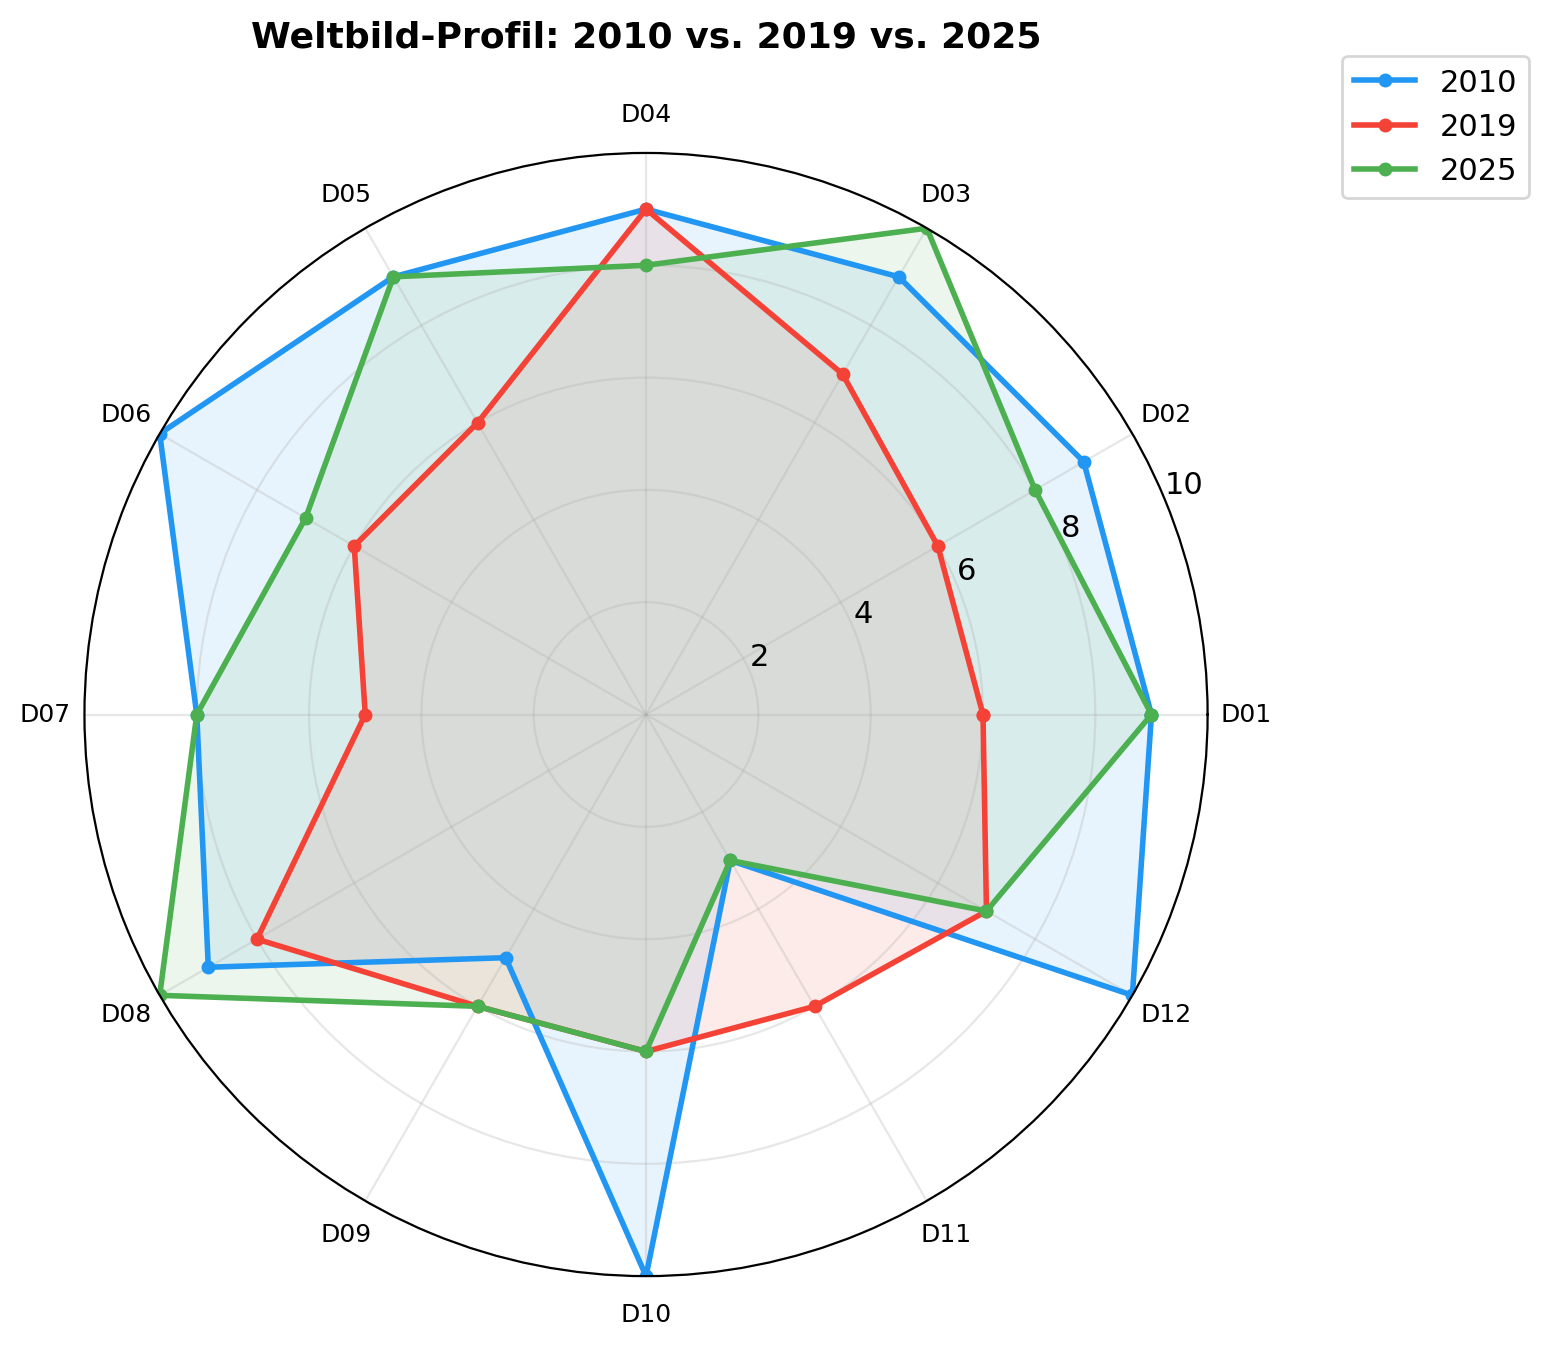
\includegraphics[width=0.85\textwidth]{fig3_radar_vergleich.png}
  \caption{Radar-Diagramm der vier Weltbild-Typen auf den 12 Dimensionen. Die Polarisierung zwischen Architekt (au\ss{}en) und H\"uter (innen) sowie die distinkte Position des Befreiers (hoher Egalitarismus bei niedriger Machtkonzentration) sind sichtbar.}
  \label{fig:radar}
\end{figure}

\medskip
\noindent\textbf{Kernbefund F4:} Die st\"arkste Polarisierung besteht zwischen Typ~I (Herrschaftslogik) und Typ~II (Teilhabelogik). Die explorative Vier-Cluster-L\"osung bedarf einer konfirmatorischen Validierung an unabh\"angigen Daten, bevor sie als robustes Ergebnis gelten kann.


\subsubsection{Algorithmische Validierung der Clusterstruktur}

Um zu pr\"ufen, ob die vier Weltbild-Typen nat\"urlichen Daten-Clustern entsprechen, wurde HDBSCAN (dichtebasiertes Clustering) und KMeans auf die $100 \times 12$-Ratingmatrix angewendet. \textbf{HDBSCAN auf dem vollen 12-dimensionalen Raum} klassifiziert 80--100\,\% der F\"alle als Rauschen \"uber alle getesteten Parameterkonfigurationen (\texttt{min\_cluster\_size} $\in \{5, 8, 10, 15\}$, \texttt{min\_samples} $\in \{3, 5\}$); die beste L\"osung findet nur 2~Cluster mit einem negativen Silhouette-Score ($-0{,}15$). KMeans mit $k = 4$ liefert einen Silhouette-Score von lediglich 0,169 -- deutlich unter dem Schwellenwert von 0,25, der typischerweise als Hinweis auf bedeutsame Struktur gilt.

\textbf{Subspace-Clustering} zeigt jedoch ein differenziertes Bild. Auf den beiden st\"arksten diskriminierenden Dimensionen (D07~Machtkonzentration und D11~Egalitarismus) identifiziert HDBSCAN mit \texttt{min\_cluster\_size}$\,=5$, \texttt{min\_samples}$\,=2$ neun Cluster mit einem \emph{Silhouette}-Score von \textbf{0,57} (12\,\% Rauschen) -- ein Hinweis auf substanzielle lokale Struktur in genau jenen Dimensionen, die die vier Idealtypen trennen. Analoges Subspace-Clustering auf den drei h\"ochstladenden PCA-Dimensionen (D02, D05, D09) ergibt einen Silhouette-Score von 0,55. Zu beachten ist allerdings eine Zirkularit\"atsproblematik: D07 und D11 sind genau jene Dimensionen, die die Architekt-Befreier-Achse in der heuristischen Typologie definieren. Das Subspace-Clustering rediskoviert dadurch teilweise das Auswahlkriterium, anstatt eine unabh\"angige Validierung zu liefern. Damit wird zwar die dimensionale Separabilit\"at best\"atigt, nicht aber die Unabh\"angigkeit der Validierung von der Typologie-Konstruktion.

Dieses Muster best\"atigt den epistemologischen Status der vier Typen: Es handelt sich um \textbf{Webersche Idealtypen} -- heuristische Verdichtungen eines mehrdimensionalen Kontinuums, nicht um emergente Daten-Cluster. Ihr analytischer Nutzen wird durch diesen Befund nicht geschm\"alert; im Gegenteil, er wird durch hochsignifikante Kruskal-Wallis-Ergebnisse \"uber die vier Typen best\"atigt (Tabelle~\ref{tab:kruskal}).

\begin{table}[htbp]
  \centering
  \caption{Kruskal-Wallis-$H$-Test \"uber die vier Weltbild-Typen ($df = 3$, $N = 100$). Signifikanz: {*}{*}{*}\,$p < 0{,}001$, {*}\,$p < 0{,}05$, n.s.\,=\,nicht signifikant. \textsuperscript{a}Nicht signifikant nach Bonferroni-Korrektur ($\alpha_{\mathrm{adj}} = 0{,}004$). Hinweis: Diese Tests beschreiben Muster innerhalb LLM-generierter Rekonstruktionen; $p$-Werte sind nominal und sollten nicht als inferenzstatistische Hypothesentests im klassischen Sinne interpretiert werden.}
  \label{tab:kruskal}
  \footnotesize
  \begin{tabular}{l c c l}
    \toprule
    \textbf{Dimension} & $H$ & $p$ & \textbf{Sig.} \\
    \midrule
    D02 Selbstwirksamkeit & 33,55 & $< 0{,}001$ & {*}{*}{*} \\
    D06 Fortschrittsglaube & 29,55 & $< 0{,}001$ & {*}{*}{*} \\
    D07 Machtkonzentration & 64,76 & $< 0{,}001$ & {*}{*}{*} \\
    D09 Menschenfreundlichkeit & 17,50 & $< 0{,}001$ & {*}{*}{*} \\
    D11 Egalitarismus & 49,57 & $< 0{,}001$ & {*}{*}{*} \\
    D12 Kontroll\"uberzeugung & 17,93 & $< 0{,}001$ & {*}{*}{*} \\
    \midrule
    D04 Verantwortungsgef\"uhl & 10,76 & 0,013 & {*}\textsuperscript{a} \\
    D05 Techno-Determinismus & 11,21 & 0,011 & {*}\textsuperscript{a} \\
    \midrule
    D01 Sendungsbewusstsein & 2,59 & 0,459 & n.s. \\
    D03 Arbeitsethos & 3,75 & 0,290 & n.s. \\
    D08 Dringlichkeit & 6,25 & 0,100 & n.s. \\
    D10 Posthumanismus & 4,04 & 0,257 & n.s. \\
    \bottomrule
  \end{tabular}
\end{table}

Nach Bonferroni-Korrektur f\"ur 12 simultane Tests ($\alpha_{\mathrm{adj}} = 0{,}05/12 = 0{,}004$) erreichen D04 ($p = 0{,}013$) und D05 ($p = 0{,}011$) nicht mehr Signifikanz. Die sechs Dimensionen mit $p < 0{,}001$ bleiben nach Korrektur signifikant. Sechs von zw\"olf Dimensionen zeigen somit hochsignifikante Inter-Typ-Unterschiede ($p < 0{,}001$), w\"ahrend zwei weitere Dimensionen (D04, D05) nominale Signifikanz auf dem $p < 0{,}05$-Niveau erreichen, aber die Bonferroni-Korrektur nicht \"uberstehen. Die vier nicht-signifikanten Dimensionen (D01, D03, D08, D10) repr\"asentieren den \emph{geteilten Kern} des KI-Elite-Weltbilds -- \"Uberzeugungen, bei denen alle vier Typen konvergieren. D07 (Machtkonzentration, $H = 64{,}76$) und D11 (Egalitarismus, $H = 49{,}57$) sind die diskriminierendsten Dimensionen. Ein Zirkularit\"atsvorbehalt gilt: Da die vier Typen teilweise \emph{durch} D07 und D11 definiert wurden, spiegeln die hohen $H$-Werte auf diesen Dimensionen teilweise das Konstruktionskriterium wider, nicht eine unabh\"angige Validierung. Die Kruskal-Wallis-Ergebnisse f\"ur die \"ubrigen Dimensionen (D02, D06, D09, D12) sind informativer, da sie nicht in die Typenkonstruktion eingingen.


\subsection{F5 -- Subgruppenvergleiche}
\label{sec:ergebnisse:f5}

Die Inter-Gruppen-Vergleiche bilden den analytischen Kern der Studie. Durch den systematischen Vergleich der kollektiven Weltbilder soziologisch definierter Gruppen -- differenziert nach institutioneller Rolle, ideologischer Haltung, Geschlecht, Firmenzugeh\"origkeit und Regulierungsposition -- deckt die Analyse auf, welche strukturellen Faktoren die kollektiven \"Uberzeugungen innerhalb der KI-Elite am st\"arksten pr\"agen. Tabelle~\ref{tab:subgruppen} ordnet die sechs diskriminierendsten Vergleiche.

\begin{table}[htbp]
  \centering
  \caption{Ranking der Subgruppen-Differenzen. $\Delta$ = Gr.~1 $-$ Gr.~2 (Durchschnitt); Einzelkontraste beziehen sich auf die Dimension mit der gr\"o\ss{}ten Abweichung.}
  \label{tab:subgruppen}
  \small
  \begin{tabular}{c l c c c l}
    \toprule
    \textbf{Rang} & \textbf{Vergleich} & \textbf{Avg Gr.~1} & \textbf{Avg Gr.~2} & $\Delta$ & \textbf{St\"arkster Kontrast} \\
    \midrule
    1 & Risiko vs.\ Speed   & 5,9 & 7,6 & 1,7 & D02, D06, D10, D12: je $-5$ \\
    2 & CEOs vs.\ Akademiker & 7,8 & 6,3 & 1,5 & D07: $+4$, D11: $-4$ \\
    3 & Frauen vs.\ M\"anner & 6,9 & 8,1 & 1,2 & D11: $-6$ \\
    4 & Open vs.\ Closed     & 6,8 & 6,3 & 0,5 & D07: $-3$, D12: $+3$ \\
    5 & Reg-Pro vs.\ Contra  & 6,3 & 6,8 & 0,5 & D04: $+4$, D06: $-3$ \\
    6 & Anthropic vs.\ OpenAI & 6,9 & 7,3 & 0,4 & D12: $-3$ \\
    \bottomrule
  \end{tabular}
\end{table}

\begin{figure}[htbp]
  \centering
  
\includegraphics[width=\textwidth]{fig5_gruppen_heatmap.png}
  \caption{Gruppen-Heatmap: 15 Subgruppen $\times$ 12 Dimensionen. Die systematische Variation von D07 (Machtkonzentration) und D11 (Egalitarismus) \"uber alle Vergleiche hinweg ist der zentrale visuelle Befund.}
  \label{fig:gruppen_heatmap}
\end{figure}

Der \textbf{st\"arkste Kontrast} (Risiko vs.\ Speed, $\Delta$~1,7) betrifft nicht die Risikoeinsch\"atzung -- beide Seiten veranschlagen die Katastrophenwahrscheinlichkeit auf 10--20\,\% --, sondern die ontologische Vorfestlegung: Risiko-Warner konzipieren KI als potenziellen autonomen Agenten, Beschleuniger als Werkzeug.

\textbf{Effektst\"arken (Cliff's $\delta$)} quantifizieren diese Kontraste nicht-parametrisch (Schwellenwerte nach \citealt{Romano2006}: $|\delta| < 0{,}147$ vernachl\"assigbar, $0{,}147$--$0{,}33$ klein, $0{,}33$--$0{,}474$ mittel, $> 0{,}474$ gro\ss{}). Die extremsten paarweisen Unterschiede zwischen den vier Weltbild-Typen treten auf der Macht-Egalitarismus-Achse auf: Architekt vs.\ Befreier ergibt $\delta = +1{,}0$ auf D07 (Machtkonzentration) und $\delta = -0{,}98$ auf D11 (Egalitarismus) -- effektiv perfekte Separation. Architekt vs.\ H\"uter erreicht $\delta = +1{,}0$ auf D07 und $\delta = -0{,}68$ auf D11. \"Uber alle sechs Cluster-Paare hinweg produzieren D07 und D11 jeweils f\"unf mittlere bis gro\ss{}e Effekte ($|\delta| \geq 0{,}33$), was sie als prim\"are Diskriminierungsdimensionen best\"atigt.

\textbf{Rollenbasierte Vergleiche} zeigen \"ahnlich starke Effekte: Akademiker vs.\ Investoren unterscheiden sich auf 9 von 12~Dimensionen mit \emph{gro\ss{}em} Effekt (am deutlichsten D02~Selbstwirksamkeit: $\delta = -0{,}88$; D12~Kontroll\"uberzeugung: $\delta = -0{,}71$; D09~Menschenfreundlichkeit: $\delta = +0{,}68$). CEOs vs.\ Akademiker zeigen gro\ss{}e Effekte auf 6~Dimensionen (D02: $\delta = +0{,}79$; D06: $\delta = +0{,}58$; D12: $\delta = +0{,}55$).

\textbf{Gender-Unterschiede} erreichen Signifikanz auf 7 von 12~Dimensionen. Die gr\"o\ss{}ten Effekte betreffen D09~Menschenfreundlichkeit ($\delta = +0{,}59$, gro\ss{}: Frauen h\"oher), D05~Techno-Determinismus ($\delta = -0{,}50$, gro\ss{}: M\"anner h\"oher) und D11~Egalitarismus ($\delta = +0{,}46$, mittel). Diese Effektst\"arken sind moderater als die nominalen Gruppenkontraste ($\Delta = 6$) vermuten lie\ss{}en, was zu erwarten ist: Cliff's $\delta$ erfasst die volle Verteilungs\"uberlappung, nicht nur Mittelwerte. Der oben genannte Kontaminationsvorbehalt gilt in vollem Umfang.

Der \textbf{gr\"o\ss{}te nominale Einzelkontrast} der gesamten Erhebung findet sich bei D11 im Gender-Vergleich: sechs volle Skalenpunkte (Frauen:~8, M\"anner:~2). Das Frauen-Weltbild ist kein Anti-Technik-Weltbild, sondern ein \emph{konditioniertes} Technik-Weltbild: gleich optimistisch, aber mit st\"arkeren ethischen Bedingungen. Dieser Befund ist jedoch der \emph{am st\"arksten kontaminationsgef\"ahrdete} der gesamten Studie und wird daher als \emph{vorl\"aufige Hypothese} eingestuft, nicht als gesicherter Befund. Die Gr\"unde: (a)~LLMs reproduzieren bekannte Gender-Stereotypen, insbesondere die Zuschreibung erh\"ohter sozialer Orientierung an Frauen \citep{Santurkar2023}; (b)~die Frauenstichprobe ist klein ($n = 18$); (c)~die Effektgr\"o\ss{}e ($\Delta = 6$) \"ubersteigt das in vergleichbaren empirischen Studien beobachtete Ausma\ss{} deutlich. Eine unabh\"angige Validierung -- idealerweise durch Replikation anderer Forschungsteams mit verschiedenen Modellen und Expertenratings -- ist f\"ur diesen Befund besonders dringlich.

Die \textbf{gr\"o\ss{}te \"Uberraschung} liegt im Regulierungsvergleich: Anti-Regulierer haben den niedrigsten Machtkonzentrations-Wert aller 15~Gruppen (D07=2). Dies widerlegt das verbreitete Narrativ, Anti-Regulierer seien Vertreter von Konzerninteressen.

\medskip
\noindent\textbf{Kernbefund F5:} Die drei st\"arksten Pr\"adiktoren f\"ur das Weltbild sind die ideologische Grundhaltung, die institutionelle Rolle und das Geschlecht. Die polarisierendsten Dimensionen sind D11 und D07. Die \emph{Machtfrage} ist der Kern der internen Differenzen.


\subsection{F6 -- Macht und Weltbild}
\label{sec:ergebnisse:f6}

\emph{Macht} wird in dieser Studie operativ als Ressourcenkontrolle verstanden: die F\"ahigkeit, \"uber Kapital, Compute-Infrastruktur, Forschungsteams und politischen Zugang zu verf\"ugen und dadurch die Richtung der KI-Entwicklung zu beeinflussen. Diese Definition folgt dem soziologischen Machtbegriff im Sinne Webers (\glqq Chance, den eigenen Willen auch gegen Widerstreben durchzusetzen\grqq) und Bourdieus (Kapitalakkumulation als Machtmechanismus), ohne eine umfassende machttheoretische Analyse zu beanspruchen.

\begin{table}[htbp]
  \centering
  \caption{Weltbild-Typen und Ressourcen-Kontrolle.}
  \label{tab:macht}
  \begin{tabular}{l c c c l}
    \toprule
    \textbf{Typ} & \textbf{Avg} & \textbf{D11} & \textbf{D04} & \textbf{Ressourcen} \\
    \midrule
    I Architekt  & 7,8 & 2,8 & 6,3 & H\"ochste \\
    III Innovator & 7,2 & 5,0 & 8,3 & Hoch \\
    IV Befreier  & 6,8 & 7,5 & 6,0 & Mittel \\
    II H\"uter   & 6,4 & 7,2 & 9,0 & Geringste \\
    \bottomrule
  \end{tabular}
\end{table}

Die Daten aus F4 (Cluster-Analyse) weiterverf\"olgend, zeigt sich ein zus\"atzliches Muster auf der Machtebene: Je h\"oher die Weltbild-Intensit\"at, desto niedriger die Werte bei Menschenfreundlichkeit und Egalitarismus und desto h\"oher die Machtkonzentrations-Akzeptanz. Das Investoren-Profil markiert den Extremfall: maximale Kontroll\"uberzeugung (D02=10) bei minimalem Verantwortungsgef\"uhl (D04=4) -- \glqq Macht ohne Rechenschaft\grqq. Das bereits in F1 beobachtete Muster (vgl.\ Abschnitt~\ref{sec:ergebnisse:f1}) versch\"arft sich: Macht intensiviert alle \"Uberzeugungen -- ausgenommen jene, die Macht selbst in Frage stellen.

\medskip
\noindent\textbf{Kernbefund F6:} Die rekonstruierten Profile zeigen ein auff\"alliges Muster: Gruppen mit h\"oherer Ressourcenkontrolle weisen intensivere Weltbild-Werte auf, bei gleichzeitig niedrigeren Werten bei Egalitarismus und Verantwortung. Da beide Seiten dieser Beobachtung auf LLM-Rekonstruktionen basieren, ist unklar, ob die Korrelation empirische Realit\"at oder interne Modellkoh\"arenz widerspiegelt. Falls robust, w\"are dies der demokratietheoretisch relevanteste Befund der Studie.


%% =============================================================================
%% ZUSAMMENFASSUNG DER KERNBEFUNDE
%% =============================================================================

\begin{table}[htbp]
  \centering
  \caption{Synopse der sechs Kernbefunde: Ergebnis, Konfidenz, Validierungsstatus und epistemischer Status. Konfidenz-Einstufung: \emph{Hoch} = stabil \"uber $\geq 3$ Gruppen-Synthesen und durch Inter-Gruppen-Konsistenz oder interne Koh\"arenzpr\"ufung gest\"utzt; \emph{Mittel-hoch} = stabil, aber ohne externe Validierung; \emph{Mittel} = explorativ, abh\"angig von Cluster-L\"osung oder kleiner Subgruppe. Epistemischer Status: (D)~=~deskriptiv, (E)~=~explorativ, (H)~=~hypothesengenerierend.}
  \label{tab:synopse}
  \footnotesize
  \begin{tabularx}{\textwidth}{l X c c c}
    \toprule
    \textbf{F} & \textbf{Kernbefund} & \textbf{Konfidenz} & \textbf{Extern val.?} & \textbf{Status} \\
    \midrule
    F1 & Technologischer Messianismus mit Ambivalenzstruktur (Avg~7,1; Doppelsenke D09/D11) & Hoch & Inter-Gruppen & (D) \\
    F2 & Utopie-Komplex erodiert; tragischer Beschleunigungszwang (D10: $-2{,}4$/Dek.) & Mittel-hoch & Nein & (D) \\
    F3 & Richtungsabh\"angige Sagen-Handeln-Kluft (D07 $+2$, D11 $-2$; stabil \"uber v1/v2) & Mittel & Nein & (H) \\
    F4 & Vier Weltbild-Typen: Architekt, H\"uter, Innovator, Befreier & Mittel & Nein & (E) \\
    F5 & St\"arkste Pr\"adiktoren: Haltung, Rolle, Gender (vorl\"aufig) & Mittel & Nein & (E) \\
    F6 & Macht-Gem\"a\ss{}igtheits-Paradox: Macht $\sim$ Extremit\"at & Hoch & Nein & (H) \\
    \bottomrule
  \end{tabularx}
\end{table}


%% =============================================================================
%% 5. DISKUSSION
%% =============================================================================
\section{Diskussion}
\label{sec:diskussion}

\subsection{Zusammenfassung und Interpretation}
\label{sec:diskussion:zusammenfassung}

Die Ergebnisse \emph{legen nahe}, dass die KI-Elite, auf Gruppenebene analysiert, ein Muster aufweist, das sich idealtypisch als \emph{technologischer Messianismus mit struktureller Ambivalenz} beschreiben l\"asst. Die Metapher des \glqq Messianismus\grqq{} ist dabei analytisch gemeint -- als Bezeichnung f\"ur die Kombination aus hohem Sendungsbewusstsein, Techno-Determinismus und Dringlichkeit --, nicht als Werturteil oder psychologisierende Zuschreibung. Der Begriff grenzt sich von verwandten Konzepten ab: \citeauthor{Morozov2013}s \glqq Solutionismus\grqq{} erfasst die Probleml\"osungshaltung, nicht die quasi-religi\"ose Dringlichkeit; \glqq Techno-Utopismus\grqq{} impliziert positiven Zukunftsglauben, der laut F2 gerade erodiert; \glqq technologischer Messianismus\grqq{} bezeichnet spezifisch die Persistenz eines erl\"oserischen Handlungsimperativs \emph{trotz} schwindendem Zukunftsoptimismus. Die sechs Forschungsfragen f\"ugen sich zu einem in sich stimmigen Bild: F1~weist auf die \glqq Doppelsenke\grqq{} bei D09 und D11 als kollektives Merkmal hin; F2~deutet auf eine Erosion des Utopie-Komplexes \"uber die Epochen hin; F3~zeigt richtungsabh\"angige Sagen-Handeln-Diskrepanzen auf spezifischen Dimensionen (D07, D11), wobei die Gesamtmagnitude der Kluft vorsichtiger Interpretation bedarf; F4~differenziert vier Weltbild-Typen mit antagonistischen kollektiven Positionen; F5 und F6 vervollst\"andigen das Bild durch das Macht-Gem\"a\ss{}igtheits-Paradox. Die Inter-Gruppen-Vergleiche (F5) bilden das analytische Herz der Studie: Der Befund, dass institutionelle Rolle, ideologische Haltung und Geschlecht die kollektiven \"Uberzeugungsstrukturen systematisch formen, tr\"agt direkte Implikationen f\"ur KI-Governance und demokratische Theorie. Alle Befunde basieren auf LLM-generierten Rekonstruktionen auf Gruppenebene und sind daher als \emph{empirisch gest\"utzte Hypothesen} zu verstehen, nicht als bewiesene Tatsachen. Formulierungen wie \glqq zeigt\grqq{} und \glqq offenbart\grqq{} sind durchg\"angig im Sinne von \glqq die Daten legen nahe\grqq{} zu lesen.

\"Uberraschend ist erstens die Richtungskonsistenz der Sagen-Handeln-Diskrepanzen \"uber Messbedingungen hinweg (D07/D11 stabil in v1 und v2); zweitens der R\"uckzug des Posthumanismus (D10 von 10 auf 6 -- widerlegt die g\"angige Annahme zunehmend posthumanistischer Orientierung); drittens die Existenz des Befreier-Typs (Opposition gegen Machtkonzentration auch von libert\"arer Seite); viertens die Konsistenz der Muster auf Gruppenebene \"uber mehrere unabh\"angige Synthesen hinweg.


\subsection{Einordnung in den Forschungsstand}
\label{sec:diskussion:einordnung}

\citeauthor{Morozov2013}s Solutionismus-These findet eine nahezu vollst\"andige Best\"atigung (D05=8--9, D06=7--9). Allerdings ist der Solutionismus kein monolithischer Block: Risiko-Warner (D05=4) teilen ihn deutlich weniger. Er ist die Ideologie des m\"achtigsten Segments, nicht der KI-Elite schlechthin.

\citeauthor{Daub2020}s Analyse der philosophischen Tiefenstrukturen wird durch die narrativen Synthesen best\"atigt. Was die vorliegende Studie hinzuf\"ugt, ist die \emph{Quantifizierung} und die Demonstration, dass sich die Intensit\"at systematisch mit der Machtposition verst\"arkt.

Die von \citet{BarbCam1996} diagnostizierte Californian Ideology findet in der Existenz des Befreier-Typs ihre zeitgen\"ossische Entsprechung -- empirisch nachweisbar drei\ss{}ig Jahre sp\"ater.

\citeauthor{Coeckelbergh2020}s Annahme einer zunehmenden Enhancement-Orientierung wird durch die rekonstruierten Trends partiell \emph{in Frage gestellt}: Der deutliche R\"uckgang des Posthumanismus (D10 von 10 auf 6) legt nahe, dass das Interesse der KI-Elite an der technologischen Transformation des Menschen selbst abgenommen hat -- zugunsten einer Fokussierung auf autonome KI-Systeme als eigenst\"andige Akteure. Dabei sind drei alternative Erkl\"arungen in Betracht zu ziehen: (a)~der R\"uckgang k\"onnte ein \emph{Diskursartefakt} sein -- posthumanistische Themen sind nach 2020 medial weniger pr\"asent, was die Datendichte entsprechender Aussagen reduziert; (b)~die Position k\"onnte nicht verschwunden, sondern in neue Begriffe transformiert worden sein (\glqq AGI\grqq{} statt \glqq Enhancement\grqq); (c)~der Trend k\"onnte eine strategische \emph{Selbstzensur} reflektieren, da posthumanistische Rhetorik politisch toxischer geworden ist.

\emph{Zum Gender-Befund.} Der in F5 berichtete extreme Kontrast bei D11 (Frauen:~8, M\"anner:~2, $\Delta = 6$) ist der gr\"o\ss{}te Einzelkontrast der gesamten Erhebung, aber zugleich der am st\"arksten kontaminationsgef\"ahrdete. LLMs reproduzieren bekannte Gender-Stereotypen -- insbesondere die Zuschreibung erh\"ohter Empathie und sozialer Orientierung an Frauen \citep{Santurkar2023}. Da die Frauenstichprobe klein ist ($n = 18$) und die Ratings vom selben LLM generiert wurden, das diese Stereotypen internalisiert hat, ist nicht unterscheidbar, ob der Kontrast (a)~eine reale Differenz in den Weltbildern, (b)~ein LLM-Stereotyp-Artefakt oder (c)~eine Mischung aus beidem reflektiert. Der Befund wird daher als \emph{Hypothese} berichtet, die einer unabh\"angigen Validierung -- idealerweise durch Replikation anderer Forschungsteams mit verschiedenen Instrumenten und Expertenratings -- bedarf.

Die von \citet{TorresGebru2024} vorgeschlagene TESCREAL-Taxonomie (Transhumanism, Extropianism, Singularitarianism, Cosmism, Rationalism, Effective Altruism, Longtermism) findet in der Vier-Cluster-L\"osung eine empirische Ausdifferenzierung: Der Architekt-Typ verk\"orpert die machtpolitische Seite des TESCREAL-B\"undels (Singularitarianism, Longtermism), der H\"uter-Typ dessen institutionelle Kritik (Effective Altruism mit Sicherheitsfokus), der Befreier-Typ den libert\"aren Extropianismus. Was die TESCREAL-Analyse als monolithisches Ideologieb\"undel beschreibt, zeigt sich in den Daten als Spektrum mit mindestens vier distinkten Positionen. \citet{Becker2025} erg\"anzt diese Perspektive durch die Analyse der \glqq Broligarchie\grqq{} als soziales Ph\"anomen: Die Verschmelzung von technologischer Vision und m\"annlicher Machtelite, die in der Gender-Analyse (F5, D11-Kontrast von 6~Skalenpunkten) ihren empirischen Niederschlag findet.

Paul Ricoeurs \glqq Hermeneutik des Verdachts\grqq{} \citep{Ricoeur1970} bietet einen erg\"anzenden analytischen Rahmen: Hinter der scheinbar neutralen, technisch-rationalen Sprachoberfl\"ache der KI-Eliten-Kommunikation verbergen sich Machtinteressen und Klassendynamiken, die erst durch systematische Dekonstruktion sichtbar werden. Die SWR-Kongruenzanalyse (F3) operationalisiert diesen Verdacht empirisch: Die $\Delta$-Werte zwischen Sagen und Handeln zeigen pr\"azise, \emph{wo} die performative Oberfl\"ache von der operativen Realit\"at abweicht.

Aus wissenschaftssoziologischer Perspektive l\"asst sich der R\"uckgang des Egalitarismus (D11) als Erosion der Merton'schen Wissenschaftsnormen lesen \citep{Merton1973}: Communalism (offener Zugang), Universalism und Organized Skepticism weichen zunehmend propriet\"aren, beschleunigungszentrierten Logiken. Der \"Ubergang von Forschungspublikation zu Produkt-Launch als prim\"arem Output-Format ist ein sichtbarer Marker dieser Verschiebung.

Die Vier-Cluster-L\"osung l\"asst sich dar\"uber hinaus feldtheoretisch lesen: Die antagonistische Struktur zwischen Architekt (\"okonomisches Kapital) und H\"uter (symbolisches Kapital) reproduziert das von \citet{Bourdieu1992} f\"ur das intellektuelle und k\"unstlerische Feld diagnostizierte Muster einer \emph{umgekehrten \"okonomischen Welt}. Im KI-Feld gilt: Wer die meisten Ressourcen kontrolliert, hat die geringste Legitimation durch Gemeinwohlorientierung -- und umgekehrt. Das Macht-Gem\"a\ss{}igtheits-Paradox (F6) l\"asst sich in dieser Perspektive als strukturelle Eigenschaft des Feldes lesen -- wobei die explorative Natur der Cluster-Daten keine konfirmatorische Aussage erlaubt.

Der spezifische Mehrwert gegen\"uber essayistischen Diagnosen liegt in drei Punkten: \emph{Masse} (100 Personen, 16 Jahre), \emph{Differenzierung} (vier distinkte Typen) und \emph{Validierung} (Kongruenzanalyse als empirischer Test).


\subsection{Agentic Alignment vs.\ Worldview Alignment}
\label{sec:diskussion:alignment}

Die in F3 angezeigten richtungsabh\"angigen Sagen-Handeln-Diskrepanzen (am robustesten: D07 Machtkonzentration $\Delta = +2$, D11 Egalitarismus $\Delta = -2$, stabil \"uber Messbedingungen) lassen sich mit einer in dieser Studie eingef\"uhrten begrifflichen Unterscheidung sch\"arfer fassen, die auf Terminologie der KI-Alignment-Debatte zur\"uckgreift.\footnote{Weder \emph{Worldview Alignment} noch \emph{Agentic Alignment} entsprechen in der hier verwendeten Bedeutung einem fest etablierten Begriff der KI-Alignment-Literatur; das Begriffspaar wird als analytische Heuristik f\"ur diese Studie eingef\"uhrt, um die performative von der operativen Ebene des Wertausdrucks zu unterscheiden.} \emph{Worldview Alignment} bezeichnet die rhetorische Reproduktion erw\"unschter Werte -- das \"offentliche Bekenntnis zu Gleichheit, Verantwortung und Menschlichkeit, wie es die \glqq Sagen\grqq-Seite der Analyse erfasst. \emph{Agentic Alignment} bezeichnet die tats\"achliche Ressourcenverteilung und Macht\-aus\"ubung -- die \glqq Handeln\grqq-Seite. Die Befunde zeigen, dass die KI-Elite ein hohes Ma\ss{} an Worldview Alignment aufweist (die \glqq richtigen\grqq{} Werte werden artikuliert), w\"ahrend das Agentic Alignment systematisch davon abweicht. Dieser Dualismus verbindet die vorliegende KI-Elite-Studie mit der breiteren Alignment-Debatte und wirft die Frage auf, ob die gegenw\"artigen Bem\"uhungen um \glqq AI Alignment\grqq{} nicht die performative Ebene (Worldview) mit der operativen (Agentic) verwechseln.


\subsection{Methodische Reflexion}
\label{sec:diskussion:methodik}

Die prim\"are Leistung der SWR liegt in der Verbindung qualitativer Tiefe mit quantitativer Systematik auf Gruppenebene. Die Studie identifiziert ein zuverl\"assiges Instrument -- Claude Opus~4.6, validiert durch Intra-Modell-Inter-Instanzen-Rating-Reliabilit\"at (IMIIRR, ICC $= 0{,}902$) -- und demonstriert dessen konsistente Anwendung \"uber alle Syntheseeinheiten. Dieser IMIIRR-Koeffizient \"ubertrifft die typische Inter-Rater-Reliabilit\"at menschlicher Kodierer in qualitativer Forschung (ICC $= 0{,}6$--$0{,}8$; \citealt{Hallgren2012}), und das Instrument bietet einen distinktiven Vorteil gegen\"uber menschlichen Kodierern: Vollst\"andig dokumentierte Prompts ersetzen implizite Kodierregeln und erm\"oglichen exakte Replikation. Die Kongruenzanalyse (F3) fungiert als interner Validit\"atstest; die Stabilit\"at des Kollektiv-Profils \"uber 15~Gruppen-Synthesen und 4~Typen st\"arkt die Konvergenzvalidit\"at. Die Inter-Gruppen-Vergleiche liefern eine eigene Form der Validierung: Wenn verschiedene Gruppensynthesen -- unabh\"angig voneinander aus unterschiedlichen Daten-Subsets produziert -- konsistente strukturelle Muster ergeben (z.\,B.\ die D07/D11-Achse als diskriminierendes Merkmal \"uber alle Vergleiche hinweg), ist dies ein Beleg f\"ur die Robustheit der Methode, der \"uber das hinausgeht, was eine einzelne Synthese leisten k\"onnte. Die Replikation mit anderen Frontier-Modellen stellt eine unabh\"angige Forschungsaufgabe dar -- analog zur Replikation einer Befragung mit verschiedenen Interviewer-Teams -- und wird explizit als Desiderat f\"ur zuk\"unftige Arbeiten identifiziert, nicht als Voraussetzung f\"ur die Validit\"at der vorliegenden Studie. Die systematische Diskussion der methodischen Grenzen -- Koh\"arenzbias, Kontaminationsrisiko, Fokuskontrolllimits, Prompt-Sensitivit\"at -- findet sich in Abschnitt~\ref{sec:limitationen}.


\subsection{Gesellschaftliche und politische Implikationen}
\label{sec:diskussion:implikationen}

Die Befunde auf Gruppenebene tragen direkte Implikationen f\"ur KI-Governance und demokratische Theorie. Das Macht-Gem\"a\ss{}igtheits-Paradox -- der systematische Befund, dass institutionelle Gruppen mit den meisten Ressourcen kollektive Weltbilder aufweisen, die am weitesten von demokratischen Idealen entfernt sind -- stellt eine konkrete Herausforderung f\"ur die Regulierungsarchitektur dar. Dieser Befund resoniert mit \citeauthor{Mills1956}' (\citeyear{Mills1956}) klassischer Analyse der \glqq Power Elite\grqq{} als sich selbst verst\"arkendes Stratum, dessen Weltbild systematisch von der breiteren \"Offentlichkeit divergiert, und best\"atigt die institutionen\"okonomische Analyse von \citet{AcemogluJohnson2023}: Technologische Eliten tendieren dazu, Innovationen so zu lenken, dass sie bestehende Machtstrukturen verst\"arken, statt sie aufzubrechen -- ein Muster, das die Autoren historisch von der Industrialisierung bis zur Digitalisierung nachzeichnen. Gegenw\"artige Governance-Ans\"atze (EU~AI~Act, Executive Order on AI) adressieren die technischen Artefakte, nicht die kollektiven Weltbilder der Gruppen, die diese Artefakte produzieren. Ein erg\"anzender Ansatz m\"usste die \emph{epistemische Diversit\"at} in KI-F\"uhrungspositionen als Regulierungsziel anerkennen.

Die systematische Sagen-Handeln-Kluft auf Gruppenebene hat eine Policy-Implikation: Freiwillige Selbstverpflichtungen -- die derzeit bevorzugte Governance-Form \citep[vgl.][]{Bengio2024} -- erscheinen unzureichend, wenn ganze institutionelle Gruppen (nicht nur vereinzelte Individuen) konsistente Diskrepanzen zwischen \"offentlicher Rhetorik und beobachtbarem Handeln aufweisen. Die Befundlage legt nahe, dass verbindliche Strukturreformen wirksamer sein d\"urften als weitere Runden freiwilliger Commitments. Drei konkrete Ansatzpunkte zeichnen sich ab: (1)~\emph{Epistemische Diversit\"atsquoten} in KI-Governance-Gremien, die sicherstellen, dass nicht nur Technologen und Investoren, sondern auch Sozialwissenschaftler, Ethikerinnen und Betroffenenvertreter an Designentscheidungen beteiligt sind; (2)~\emph{verpflichtende Weltbild-Audits} f\"ur KI-Unternehmen ab einer bestimmten Gr\"o\ss{}e, analog zu Nachhaltigkeitsberichten; (3)~\emph{st\"arkere Entkopplung} von Kapitalgebern und Forschungssteuerung, beispielsweise durch \"offentlich finanzierte KI-Labore mit unabh\"angiger Governance \citep[vgl.][]{AcemogluJohnson2023}.

Die Inter-Gruppen-Vergleiche offenbaren ein weiteres governance-relevantes Muster: Die Frage der Macht (D07) und der Gleichheit (D11) ist die Achse, entlang derer sich s\"amtliche Gruppenunterschiede organisieren. Ob CEOs mit Akademikern, Beschleuniger mit Risiko-Warnern oder M\"anner mit Frauen verglichen werden -- die Macht-Gleichheits-Achse ist durchg\"angig die diskriminierendste Dimension. Dies legt nahe, dass die zentrale ideologische Bruchlinie innerhalb der KI-Elite nicht die Technik betrifft (alle Gruppen sind technologisch optimistisch), sondern die \emph{Verteilung} technologischer Macht.

Ist sich die KI-Elite ihrer eigenen blinden Flecken bewusst? Das Verantwortungsgef\"uhl (D04=7) ist nicht absent, aber funktional eingebettet: Es legitimiert das Weiterarbeiten, nicht das Innehalten. Der Befund, dass demokratische Langsamkeit durchg\"angig als Hindernis, nicht als Schutzfunktion begriffen wird, markiert den gravierendsten blinden Fleck einer Gruppe, die dar\"uber entscheidet, wie Milliarden Menschen in Zukunft leben werden.


\subsection{Was die Studie nicht zeigt}
\label{sec:diskussion:negativ}

Zur Vermeidung h\"aufiger Fehlinterpretationen sei explizit festgehalten, was die vorliegende Studie \emph{nicht} leistet: (1)~keine \emph{Kausalerkl\"arung} (vgl.\ Abschnitt~\ref{sec:limitationen}); (2)~keine \emph{individuellen Profile} -- die 100~Akteure dienen als Datenlieferanten; die Analyseeinheiten sind soziologisch definierte Gruppen; die Ratings sind kollektive Abstraktionen auf Gruppenebene, keine Pers\"onlichkeitsprofile oder individuelle Biographien; (3)~keine \emph{Vorhersagen} \"uber k\"unftiges Verhalten -- die Weltbilder beschreiben den Zeitraum 2010--2026; (4)~keine \emph{repr\"asentative Stichprobe} im statistischen Sinne (vgl.\ Abschnitt~\ref{sec:limitationen}); (5)~kein Beweis, dass die \emph{Sagen-Handeln-Kluft} auf bewusste T\"auschung zur\"uckgeht -- alternative Erkl\"arungen (institutionelle Zw\"ange, kognitive Dissonanz, rollenspezifische Kommunikation) sind gleicherma\ss{}en plausibel.


%% =============================================================================
%% 6. LIMITATIONEN
%% =============================================================================
\section{Limitationen}
\label{sec:limitationen}

Tabelle~\ref{tab:validation_overview} gibt einen kompakten \"Uberblick \"uber die identifizierten methodischen Probleme, ergriffene Gegenma\ss{}nahmen und deren Ergebnisse. Die detaillierte Diskussion folgt in den Unterabschnitten.

\begin{table}[htbp]
  \centering
  \caption{Validierungs\"ubersicht: Methodische Probleme, Gegenma\ss{}nahmen und Ergebnisse.}
  \label{tab:validation_overview}
  \scriptsize
  \begin{tabular}{@{} p{2.4cm} p{1.4cm} p{4.2cm} p{4.5cm} p{1.0cm} @{}}
    \toprule
    \textbf{Problem} & \textbf{Typ} & \textbf{Gegenma\ss{}nahme} & \textbf{Ergebnis} & \textbf{Ref.} \\
    \midrule
    LLM-Kontamination & Design & Fokuskontrolle (Anonym.\ + Aufgabenfokus) & Var.\,C: MAE\,=\,0,67 & QA\,(e) \\[3pt]
    Anthropic-Zirkularit\"at & Antizipiert & Matched-Sample ($n$\,=\,9 vs.\ 9) & MAE\,=\,1,00, kein Bias & QA\,(h) \\[3pt]
    Erwartungs-Diskrepanz & Post hoc & Instanztrennung (v2-Protokoll) & Gap $-47\%$; Gruppen-Gaps bestehen & QA\,(g) \\[3pt]
    Rating-Instabilit\"at & Antizipiert & IMIIRR ($N$\,=\,15 unabh.\ Runs) & ICC(3,1)\,=\,0,847, Mean~SD\,=\,0,45 & QA\,(a) \\[3pt]
    Reihenfolge-Effekt & Antizipiert & Permutationstest (2 Reihenfolgen) & 12/12 identisch & QA\,(f) \\[3pt]
    Koh\"arenzbias & Antizipiert & Ausrei\ss{}er-Detektion + Inversionskontrolle & 80--88\% Passung; 58\% $\Delta$\,$\geq$\,5 & QA\,(i,j) \\[3pt]
    Artefaktische Sagen-Handeln-Kluft & Antizipiert & G6-Kontrollkorpus & v2-Baseline MAE\,=\,0,92 & QA\,(b) \\[3pt]
    Kreuzmodale Validit\"at & Antizipiert & Op4-Vorhersage (5 Gruppen) & 72\% best\"atigt, 0\% widerlegt & QA\,(d) \\[3pt]
    Aggregationsverzerrung & Antizipiert & Direkt vs.\ aggregiert Vergleich & $r$\,=\,0,623, Amplifikationseffekt & QA\,(c) \\[3pt]
    Einflussgradient & Post hoc & Strata-Vergleich (3 Rangstufen) & Gradient best\"atigt; D09/D10 invers & QA\,(k) \\[3pt]
    Statist.\ Power & Abgeschlossen & $N$\,=\,15 unabh.\ Opus-Runs & Mean~SD\,=\,0,45; Batch-1 in CI: 3/12 & QA\,(a) \\[3pt]
    Modellsensitivit\"at & Desiderat & Inter-Modell-Vergl.\ (unabh.\ Runs) & Zuk\"unftige Arbeit & \S\,\ref{sec:limitationen} \\
    \bottomrule
  \end{tabular}
\end{table}

\subsection{Datenbezogene Limitationen}

\emph{Quellenbias.} Die Datenbasis beschr\"ankt sich auf \"offentliche Aussagen und beobachtbare Handlungen. Die rekonstruierten Weltbilder spiegeln das \emph{\"offentlich dargebotene} Weltbild wider, nicht das \emph{tats\"achlich geglaubte}. Die Aussagen-Handlungen-Vergleichsanalyse (F3) bietet ein partielles Korrektiv, kann das Problem aber nicht eliminieren.

\emph{Zeitliche Ungleichverteilung.} Die Datendichte variiert um Faktor ${\sim}43$: von 17~Datenpunkten im Jahr 2010 bis 735 im Jahr 2024. F\"ur 2010--2015 liegen 2--5 Aussagen pro Person vor, f\"ur 2023--2026 dagegen 30--80. Das Kriterium K2 (Mindestgr\"o\ss{}e~15) und dokumentierte Zusammenlegungen mildern das Problem, und alle Jahres-Syntheseeinheiten erf\"ullen den Mindestschwellenwert; fr\"uhere Zeitreihen beruhen dennoch auf d\"unnerer Evidenz und sollten mit gr\"o\ss{}erer Unsicherheit interpretiert werden.

\emph{Westlicher und Sprachbias.} Die Stichprobe ist \"uberproportional angloamerikanisch gepr\"agt. Chinesische, japanische und s\"udkoreanische KI-Pers\"onlichkeiten sind unterrepr\"asentiert. Die Befunde gelten prim\"ar f\"ur die westliche KI-Elite.

\emph{Stichprobenabh\"angigkeit.} Die Auswahl der 100~Personen erfolgte durch den Autor mittels eines mehrstufigen, aber letztlich subjektiven Scoring-Verfahrens. Eine intersubjektive Validierung der Stichprobenzusammensetzung (z.\,B.\ durch unabh\"angige Expertenpanels) steht aus. Da die Befunde sensitiv gegen\"uber der Stichprobenzusammensetzung sein k\"onnten, ist eine Replikation mit alternativen Auswahlverfahren w\"unschenswert.


\subsection{Methodische Limitationen}

\emph{LLM-Kontamination und Fokuskontrollgrenzen.} Trotz konsequenter Fokuskontrolle kann nicht ausgeschlossen werden, dass das LLM auf Trainingswissen zur\"uckgreift. Die Fokuskontrolle operiert auf zwei Ebenen: (1)~\emph{Anonymisierung} -- Ersetzung aller identifizierenden Informationen durch neutrale Platzhalter, sodass das Modell nicht an spezifischen Individuen ankern kann -- und (2)~\emph{Aufgabenfokus} -- das Prompt-Design lenkt das Modell darauf, ein koh\"arentes Weltbild aus den pr\"asentierten Daten zu synthetisieren, ohne Verblindung, Identit\"at oder die Existenz versteckter Informationen zu erw\"ahnen (v2-Prompts, siehe Repository). Ein empirischer Test der Anonymisierungskomponente best\"atigte, dass die Wahl der Verblindungsstrategie (Platzhalter-Tokens vs.\ fiktive Namen) keinen wesentlichen Effekt auf Ratings auf Gruppenebene hat ($r = 0{,}987$, MAE $= 0{,}33$, max $|\Delta| = 1$; siehe Abschnitt~\ref{sec:methodik:qualitaet}). Eine dritte Variante~(C) testete die vollst\"andige Identit\"atsoffenlegung -- dieselbe Syntheseeinheit wurde mit den echten Namen aller Gruppenmitglieder verarbeitet (Musk, Sutskever, Hinton, Russell, Bengio, Leike). Das Ergebnis zeigte einen moderaten, aber nicht drastischen Effekt: A--C MAE $= 0{,}67$, $r = 0{,}850$, bei identischem Gruppendurchschnitt (7,1). Die gr\"o\ss{}te Verschiebung betraf D11~(Egalitarismus, $+2$ Punkte). Dies best\"atigt, dass Anonymisierung einen messbaren, aber bescheidenen Schutz bietet; das kollektive Weltbild ist weitgehend stabil, auch wenn Identit\"aten bekannt sind. Entscheidend ist nicht, ob das Modell Individuen erkennt, sondern ob es seine Aufgabe erf\"ullt: eine koh\"arente Synthese auf Gruppenebene aus den bereitgestellten Daten zu konstruieren. Auf Gruppenebene ist das Kontaminationsrisiko strukturell reduziert, da kein LLM-Trainingskorpus vorgeformte kollektive Weltbilder soziologischer Gruppen enth\"alt.

\emph{Anthropic-interne Zirkularit\"at.} Ein besonders zugespitzter Fall des Zirkularit\"atsproblems betrifft die Synthese auf Gruppenebene f\"ur Subgruppen, die Personen enthalten, die direkt an der Entwicklung des verwendeten LLM beteiligt sind. Claude Opus~4.6 wird von Anthropic entwickelt; mehrere Anthropic-F\"uhrungskr\"afte (z.\,B.\ Dario Amodei, Daniela Amodei) geh\"oren zur analysierten Stichprobe und ihre Daten flie\ss{}en in die Gruppensynthesen ein. Um systematische Verzerrungen zu testen, wurde eine Matched-Sample-Kontrolle durchgef\"uhrt: Die Anthropic-Subgruppe ($n = 9$) wurde mit einer gematchten Kontrollgruppe nicht-Anthropic-affiliierter Gr\"under und Forscher ($n = 9$, gleiche Gr\"o\ss{}e und Rollenkomposition) verglichen. Die resultierenden Profile zeigten MAE $= 1{,}00$ ohne Dimensions-Differenz $|\Delta| \geq 3$. Die beobachteten Unterschiede -- Anthropic-Mitglieder mit h\"oherer Dringlichkeit (D08) und Machtkonzentration (D07), die Kontrollgruppe mit h\"oherem Posthumanismus (D10) und Kontroll\"uberzeugung (D12) -- sind als genuine Gruppenunterschiede interpretierbar, die Anthropics Safety-orientierte Kultur widerspiegeln, nicht als Modellverzerrung. W\"ahrend dieser Within-Model-Test Zirkularit\"at nicht vollst\"andig ausschlie\ss{}en kann (eine Cross-Model-Replikation bleibt als externe Validierung w\"unschenswert), liefert er keinen Beleg f\"ur systematische Anthropic-spezifische Verzerrung.

\emph{Kritik synthetischer Personas.} Die wachsende Literatur zu LLM-generierten synthetischen Personas mahnt zur Vorsicht, aber die Kritik muss sorgf\"altig eingegrenzt werden. \citet{Santurkar2023} zeigt, dass LLMs Meinungen spezifischer demografischer Gruppen systematisch verfehlen und \glqq WEIRD\grqq-Verzerrungen aufweisen, wenn sie als \emph{Meinungsgeneratoren} eingesetzt werden -- d.\,h.\ wenn sie aufgefordert werden zu simulieren, was eine demografische Gruppe denken k\"onnte. Ebenso finden \citet{Argyle2023}, dass synthetische Agenten Leitthemen erfassen, aber an authentischer Tiefe realer Diskurse scheitern, wenn sie qualitative Daten \emph{generieren}. Ein aktuelles systematisches Review von 63 Peer-reviewed-Persona-Experimenten (2023--2025) best\"atigt dieses Muster: Die meisten Studien spezifizieren die Zielpopulation unzureichend, nur 35\,\% adressieren Repr\"asentativit\"at, und die \"okologische Validit\"at ist durchg\"angig gering \citep{Batzner2025WhosePersonae}. Diese Kritiken zielen auf einen fundamental anderen Anwendungsfall als die SWR. In der vorliegenden Studie generiert das LLM keine Meinungen; es \emph{verdichtet} 3.132 reale Datenpunkte (dokumentierte Aussagen und Handlungen) in strukturierte Profile auf Gruppenebene. Die synthetische Persona ist ein analytisches Verdichtungsinstrument -- n\"aher am Weber'schen Idealtyp als am Simulationsagenten. Die von \citeauthor{Santurkar2023} identifizierte WEIRD-Verzerrung ist weitgehend orthogonal: Die KI-Elite \emph{ist} eine westliche, gebildete, wohlhabende und industrialisierte Population, sodass jede demographische Schieflage in den Vorannahmen des Modells mit der Zielgruppe konvergiert, anstatt sie zu verzerren. Dennoch bleibt die Tendenz zur \"Uberrepr\"asentation \"offentlich dominanter Narrative und zur Unterrepr\"asentation idiosynkratischer oder widerspr\"uchlicher Positionen eine genuine Limitation.

\emph{Quantifizierung und interne Konsistenz.} Die in Abschnitt~\ref{sec:ergebnisse:f2} berichteten Dimensionskorrelationen (z.\,B.\ $r_s = +0{,}85$ zwischen D10 und D12) werden innerhalb des Rating-Prozesses des LLM generiert und k\"onnten teilweise interne Konsistenz statt empirischer Zusammenh\"ange widerspiegeln. Dieses Problem betrifft spezifisch den \emph{Rating-Schritt} (Op2) und gilt f\"ur jedes Rating-Verfahren einschlie\ss{}lich menschlicher Rater: Ein menschlicher Kodierer, der Posthumanismus hoch bewertet, wird durch kognitive Koh\"arenz auch Kontroll\"uberzeugung tendenziell hoch bewerten. Das Problem betrifft \emph{nicht} die qualitativen Synthesen (Op1), die ohne dimensionales Prompting direkt aus den Rohdaten generiert werden. Mehrere Validierungsergebnisse begrenzen die Reichweite dieser Limitation: (1)~Die kreuzmodale Vorhersage (G5, 72\,\% best\"atigt) zeigt, dass LLM-rekonstruierte Muster empirische Substanz haben -- aus Aussagen abgeleitete Vorhersagen wurden durch unabh\"angig evaluierte Handlungen best\"atigt; (2)~der Reihenfolge-Invarianztest zeigt, dass die Ratings nicht von der Pr\"asentationsreihenfolge der Dimensionen abh\"angen; (3)~die IMIIRR-Koeffizienten (ICC $= 0{,}902$ aus $5 \times 2$ Runs; ICC $= 0{,}847$ aus $N = 15$ unabh\"angigen Einzelinstanz-Runs) etablieren, dass das Rating-Verfahren stabil und reproduzierbar ist. Die berichteten Korrelationen sind als Muster eines zuverl\"assig kalibrierten Rekonstruktionsinstruments zu lesen, nicht als Artefakte willk\"urlichen Modellverhaltens -- eine externe Replikation bleibt jedoch w\"unschenswert zur Best\"atigung, welche spezifischen Korrelationen \"uber Instrumente hinweg bestehen.

\emph{Statistische Power.} Eine formale Power-Analyse wurde an einer Gruppen-Syntheseeinheit (GA\_ges\_AH) mit $N = 15$ vollst\"andig unabh\"angigen Opus-Instanzen (je ein separater Agent ohne geteilten Kontext) durchgef\"uhrt. Die Ergebnisse zeigen, dass das Instrument hochstabil ist: mittlere SD $= 0{,}45$ \"uber alle 12~Dimensionen (Bereich: 0,00--0,74), mit 95\,\%-Konfidenzintervallen schmaler als $\pm 0{,}5$ Skalenpunkte f\"ur die meisten Dimensionen. Der urspr\"ungliche Batch-1-Einzelwert lag nur in 3 von 12 Konfidenzintervallen (MAE zum $N = 15$-Mittelwert $= 0{,}73$), was best\"atigt, dass Einzelmessungen unzuverl\"assig sind und $N \geq 15$ unabh\"angige Runs f\"ur robuste Profilsch\"atzungen erforderlich sind. Die Analyse wurde jedoch an einer einzelnen Syntheseeinheit durchgef\"uhrt; die Generalisierung auf alle 56~SEs bleibt ein Desiderat f\"ur zuk\"unftige Arbeiten. Die berichteten $\Delta$-Werte, Korrelationen und Cluster-Unterschiede auf Gruppenebene sind deskriptive Muster in rekonstruierten Daten; die Interpretation beruht auf inhaltlicher Einordnung, informiert durch die bekannte Messpr\"azision.

\emph{Reproduzierbarkeit.} LLM-Outputs sind auch bei Temperatur~0 nicht vollst\"andig deterministisch. Die urspr\"unglichen Synthesen wurden in Einzeldurchl\"aufen pro SE generiert. Zwei Post-hoc-IMIIRR-Validierungen etablieren die Reproduzierbarkeit: (1)~f\"unf Gruppen-Syntheseeinheiten, je zweimal verarbeitet, ergaben ICC $= 0{,}902$, MAE $= 0{,}40$ ($\pm 0{,}2$ Skalenpunkte); (2)~$N = 15$ vollst\"andig unabh\"angige Einzelinstanz-Runs auf einer Syntheseeinheit ergaben ICC(3,1) $= 0{,}847$, mittlere SD $= 0{,}45$, wobei eine Dimension (D02) perfekte \"Ubereinstimmung \"uber alle 15~Instanzen zeigte. Beide Intra-Instrument-Reliabilit\"atssch\"atzungen \"ubertreffen die typische Inter-Rater-\"Ubereinstimmung menschlicher Kodierer in qualitativer Forschung (ICC $= 0{,}6$--$0{,}8$; \citealt{Hallgren2012}), was best\"atigt, dass das LLM-basierte Instrument einen \emph{Reproduzierbarkeits\-vorteil} gegen\"uber konventioneller Kodierung bietet. Ob verschiedene Modelle desselben oder anderer Anbieter auf \"ahnliche Profile konvergieren, bleibt eine offene Frage --- ein Inter-Modell-Vergleich mit strikten Unabh\"angigkeitskriterien (separater Agent pro Run, kein geteilter Kontext) wird als Priorit\"at f\"ur zuk\"unftige Replikation identifiziert.

\emph{Daten-Bias in der Sagen-Handeln-Rekonstruktion.} Die der SWR-Methode verf\"ugbaren Daten sind strukturell asymmetrisch: \"Offentliche Aussagen sind reichhaltig und explizit, w\"ahrend Handlungen aus dokumentierten Entscheidungen, Investitionen und organisatorischem Verhalten erschlossen werden m\"ussen. Diese Asymmetrie bedeutet, dass die \glqq Sagen\grqq-Seite auf dichterer Evidenz beruht als die \glqq Handeln\grqq-Seite. Der Trainingskorpus des LLM spiegelt dieselbe Asymmetrie wider -- \"offentlicher Diskurs ist relativ zu dokumentiertem operativem Verhalten \"uberrepr\"asentiert. Diese Datenlimitation ist besonders relevant f\"ur den Sagen-Handeln-Vergleich, bei dem das Handlungsprofil weniger pr\"azise kalibriert sein k\"onnte als das Aussagenprofil. Die robusten Richtungsbefunde (D07 Machtkonzentration, D11 Egalitarismus) persistieren \"uber Messbedingungen hinweg, aber ihre Magnitude sollte angesichts dieser strukturellen Asymmetrie konservativ interpretiert werden. Die Limitation ist der Datenstruktur inh\"arent, nicht der Methode: Jeder Analyst -- menschlich oder algorithmisch --, der auf \"offentliche Quellen angewiesen ist, w\"urde derselben Evidenzasymmetrie begegnen.

\emph{Erwartete-Diskrepanz-Bias.} Die Kongruenzanalyse (F3) vergleicht zwei LLM-Synthesen -- eine aus Aussagen, eine aus Handlungen --, die beide vom selben Modell generiert wurden. Da LLMs auf sozialwissenschaftlicher Literatur trainiert sind, in der Sagen-Handeln-Diskrepanzen bei Eliten als Standardbefund gelten, ist ein Erwartungseffekt plausibel: Das Modell k\"onnte die \emph{erwartete} Diskrepanz reproduzieren, statt sie empirisch zu entdecken. Diese Studie liefert Evidenz, dass der Effekt \emph{existiert}, aber \emph{kontrollierbar} ist. Die urspr\"ungliche Analyse (v1), bei der beide Datentypen in derselben LLM-Instanz verarbeitet wurden, ergab eine Gesamtkluft von MAE $= 1{,}42$. Bei Wiederholung mit strikter Instanztrennung (v2-Protokoll) -- jeder Datentyp von einem unabh\"angigen Agenten ohne geteilten Kontext verarbeitet -- schrumpfte die Gesamtkluft auf MAE $= 0{,}75$ ($-47\,\%$). Diese Reduktion zeigt, dass geteilter Kontext die Kluft \emph{tats\"achlich} verst\"arkt hat, was die Erwartungs-Diskrepanz-Bedenken als empirisch real best\"atigt. Die Gegenma\ss{}nahme (Instanztrennung) ist jedoch wirksam: Die v2-Kluft f\"allt unter die Kontrollbaseline (MAE $= 0{,}92$, einer fiktiven konsistenten Gruppe unter gleichen Bedingungen), was darauf hindeutet, dass die aggregierte Kluft nicht mehr zuverl\"assig von Messrauschen unterscheidbar ist. Der methodisch entscheidende Befund ist, dass \emph{gruppenspezifische} Gaps die Korrektur \"uberstehen: CEOs (MAE $= 1{,}08$) und Risiko-Warner (MAE $= 1{,}92$) \"uberschreiten die Baseline auch unter v2-Bedingungen, mit stabilen Richtungsmustern (D07, D11 f\"ur CEOs; D09, D10 f\"ur Risiko-Warner). Der Erwartete-Diskrepanz-Bias ist somit ein reales methodisches Problem, das in dieser Studie identifiziert, quantifiziert und teilweise kontrolliert wurde -- keine unadressierte Limitation.

\emph{Koh\"arenzbias.}\footnote{Der Begriff \emph{Koh\"arenzbias} wird in dieser Studie als operativer Arbeitsbegriff verwendet; kein etabliertes Konzept dieses genauen Namens wurde in der methodischen Literatur gefunden. Das zugrundeliegende Ph\"anomen --- die Tendenz von LLMs, logisch koh\"arente Synthesen zu produzieren, die echte Inkonsistenz in den Quelldaten gl\"atten k\"onnen --- wird empirisch durch die in Abschnitt~\ref{sec:methodik:qualitaet} beschriebenen Abweichungsdetektions- und Inversionskontrollmechanismen adressiert.} LLMs sind auf logische Koh\"arenz optimiert; Menschen sind von Natur aus inkonsistent. F\"ur die Weltbild-Rekonstruktion ist diese Eigenschaft zugleich operativer Vorteil und Quelle systematischer Verzerrung. Der Vorteil: Koh\"arenz erm\"oglicht es der SWR, aus heterogenen Daten stabile, interpretierbare Profile auf Gruppenebene zu extrahieren -- die Methode \emph{nutzt} Koh\"arenz als Kompressionsmechanismus, analog dazu, wie Faktoranalyse Kovarianzstruktur nutzt. Die Verzerrung: Die resultierenden Cluster-Typen (Architekt, H\"uter, Innovator, Befreier) k\"onnten sch\"arfer konturiert erscheinen, als sie in der Realit\"at sind. Die interne Spannung, die reale Personen zwischen z.\,B.\ Machtstreben und Verantwortungsgef\"uhl erleben, wird vom LLM zugunsten eines konsistenten Profils aufgel\"ost. Die genuine Limitation ist daher \emph{\"Uber-Koh\"arenz}: Cluster sch\"arfer als die empirische Realit\"at. Zwei Kontrollmechanismen adressieren dieses Risiko teilweise: (1)~die in die SWR-Pipeline eingebaute Abweichungsdetektion ergibt eine Passung auf Gruppenebene von 80--88\,\%, nicht 100\,\%, was darauf hindeutet, dass das Modell Heterogenit\"at innerhalb der Gruppe registriert und bewahrt; und (2)~die Inversionskontrolle (Op3, Kongruenzanalyse) zeigt, dass 58\,\% der Dimensionen $|\Delta| \geq 5$ aufweisen, was demonstriert, dass die Methode substanzielle Diskrepanzen nicht gl\"attet.


\subsection{Konzeptuelle Limitationen}

\emph{Aggregation als Design-Merkmal.} Kollektive Synthesen nivellieren individuelle Variation -- dies ist die intendierte Funktion der Methode, kein Nebenprodukt. Die Forschungsfragen der Studie (F1--F6) sind auf Gruppenebene formuliert; individuelle Variation ist relativ zu diesem analytischen Ziel Rauschen, ebenso wie Individualebene-Varianz in jeder Aggregatanalyse Rauschen darstellt (nationale Surveys, Branchenbenchmarks, Metaanalysen). Die algorithmische Strukturpr\"ufung (PCA, HDBSCAN; Abschnitt~\ref{sec:ergebnisse:f4}) best\"atigt, dass die Individualebene-Ratingmatrix genuine strukturelle Variation \emph{vor} der Aggregation aufweist, was darauf hindeutet, dass die Muster auf Gruppenebene Kompressionen realer Heterogenit\"at sind, nicht Artefakte uniformer Eingabedaten.

\emph{Keine Kausalerkl\"arung.} Die Studie identifiziert, \emph{was} die KI-Elite kollektiv glaubt, und dokumentiert zeitliche Assoziationen (F2: L\"angsschnitttrends) und strukturelle Kovariationen (F5: Gruppenunterschiede korreliert mit Rolle, Haltung und Geschlecht). Sie etabliert keine kausalen Mechanismen. Die zeitliche Abfolge von Weltbild-Verschiebungen und die systematische Kovariation mit struktureller Position liefern plausible assoziative Evidenz, aber der Ausschluss von Drittvariablen-Erkl\"arungen w\"urde andere Forschungsdesigns erfordern (L\"angsschnitt-Panelstudien, nat\"urliche Experimente oder biographische Fallanalysen).

\emph{Epistemologische Grenzen der Quantifizierung.} Die dimensionalen Bewertungen (Skala 1--10) bieten ein handhabbares Format f\"ur Aggregation und Vergleich, setzen aber eine Kommensurabilit\"atsannahme voraus, die explizite Reflexion verdient. Komplexe normative Orientierungen -- wie etwa \emph{Kontrollverantwortung \"uber KI} (D07) oder \emph{Posthumanismus} (D10) -- sind mehrdimensionale Konstrukte, die sich nicht sauber auf eine einzige geordnete Dimension abbilden lassen. Die numerische Zuweisung ist am besten als \emph{ordinale Kompression} zu verstehen: ein zusammenfassendes Urteil \"uber die relative Position, keine Messung einer zugrundeliegenden Gr\"o\ss{}e. Drei Einschr\"ankungen folgen daraus. Erstens sind Interpretationen auf Intervallniveau nicht gerechtfertigt; die berichteten Spearman-Korrelationen und rangbasierte Clusteranalyse respektieren diese Einschr\"ankung. Zweitens impliziert die Zuweisung eines einzelnen Werts je Dimension ein Ma\ss{} an \emph{Reifikation}: die Abstraktion einer vielstr\"angigen diskursiven Orientierung auf einen Punkt einer Skala. Die qualitative Synthese (Op1) bewahrt die Nuance, die die Bewertung (Op2) komprimiert. Drittens sind die 12~Dimensionen konzeptuell distinkt, aber empirisch interkorreliert (z.\,B.\ $r_s = +0.85$ f\"ur D10--D12); ein Teil dieser Kovariation k\"onnte echte Konstrukt-\"Uberlappung widerspiegeln, nicht unabh\"angige empirische Beziehungen. Diese Einschr\"ankungen sind in jeder quantitativen Weltbildforschung angelegt und nicht spezifisch f\"ur die SWR-Methode; sie mahnen zu Zur\"uckhaltung bei feink\"ornigen numerischen Vergleichen, lassen aber die Richtungsmuster und strukturellen Kontraste -- die prim\"aren Aussagen der Studie -- unber\"uhrt.

\subsection{Forschungsethische Reflexion}

Die Studie analysiert \"offentliche Figuren ausschlie\ss{}lich auf der Grundlage \"offentlich zug\"anglicher Daten. Zwei Design-Merkmale mildern ethische Bedenken substanziell.

\emph{Aggregation auf Gruppenebene als ethischer Schutz.} Die prim\"aren Analyseeinheiten sind soziologisch definierte Gruppen, nicht Individuen. Individuelle Daten werden vor der Synthese in Gruppenkorpora gepoolt; kein individuelles Weltbild-Profil wird als Befund berichtet. Die rekonstruierten Weltbilder beschreiben kollektive Tendenzen von Rollen (CEOs, Akademiker) und Haltungen (Beschleuniger, Risiko-Warner), nicht die Psychologie identifizierbarer Personen. Diese Aggregation verhindert strukturell die Zuschreibung spezifischer \"Uberzeugungen an namentlich genannte Individuen.

\emph{Standard-Legitimation.} Die Studie st\"utzt sich auf \"offentlich dokumentierte berufliche Aussagen und Handlungen \"offentlicher Figuren, deren Positionen zur KI-Entwicklung von erheblichem \"offentlichem Interesse sind (vgl.\ APA Ethical Principles, Standard~8.05). Keine privaten oder vertraulichen Informationen wurden erhoben.

\emph{Residualrisiko.} F\"ur kleine Gruppen (z.\,B.\ firmenspezifische Subgruppen mit $n = 3$--5) bietet die Aggregation schw\"acheren Schutz -- ein quasi-individuelles Profil kann entstehen. Die drei individuellen Spot-Checks (Abschnitt~\ref{sec:limitationen:spotchecks}) werden als Datenqualit\"atsindikatoren pr\"asentiert, nicht als inhaltliche Befunde. Member Checking \citep{SoysalTurkmen2024} bleibt ein Desiderat f\"ur Folgeforschung.


\subsection{Individualebene-Analyse (explorativ)}
\label{sec:limitationen:spotchecks}

Die inhaltlichen Befunde der Studie beruhen vollst\"andig auf Analysen auf Gruppenebene (F1--F6). SWR auf Individualebene ist f\"ur den vorliegenden Zweck methodisch \"uberfl\"ussig -- die originalen \"offentlichen Aussagen und Handlungen sind f\"ur jede Einzelperson direkt zug\"anglich. Der Mehrwert der SWR liegt ausschlie\ss{}lich in der Synthese auf Gruppenebene, wo sie kollektive Portr\"ats erzeugt, die in keiner einzelnen Quelle existieren. Die folgenden drei Spot-Checks werden ausschlie\ss{}lich als \emph{Datenqualit\"atsindikatoren} berichtet: Wenn die zugrundeliegenden Individualdaten erkennbare, verifizierbare Profile produzieren, st\"utzt dies die Qualit\"at der Eingabedaten f\"ur die Gruppensynthesen. Tabelle~\ref{tab:spotchecks} fasst die Ergebnisse zusammen.

\begin{table}[htbp]
  \centering
  \caption{Explorative Validierung auf Individualebene: SWR-Ratings vs.\ dokumentierte Positionen. Diese Einzelfallpr\"ufungen dienen als Plausibilit\"atstests f\"ur die zugrundeliegende Datenqualit\"at; die inhaltlichen Befunde der Studie beruhen auf den Gruppenanalysen (F1--F6).}
  \label{tab:spotchecks}
  \footnotesize
  \begin{tabularx}{\textwidth}{l c l c l c l}
    \toprule
    & \multicolumn{2}{c}{\textbf{Sam Altman}} & \multicolumn{2}{c}{\textbf{Geoffrey Hinton}} & \multicolumn{2}{c}{\textbf{Marc Andreessen}} \\
    \textbf{Dim.} & \textbf{R} & \textbf{Status} & \textbf{R} & \textbf{Status} & \textbf{R} & \textbf{Status} \\
    \midrule
    D01 Send. & 9 & best. & 7 & best. & 8 & best. \\
    D02 Selbst. & 9 & best. & 5 & best. & 9 & best. \\
    D03 Arbeit & 9 & best. & 7 & plaus. & 8 & best. \\
    D04 Verantw. & 6 & best. & 10 & best. & 4 & best. \\
    D05 Techno. & 9 & best. & 6 & best. & 9 & best. \\
    D06 Fortschr. & 8 & best. & 4 & best. & 9 & best. \\
    D07 Macht & 9 & best. & 4 & best. & 2 & best. \\
    D08 Dringl. & 9 & best. & 10 & best. & 7 & plaus. \\
    D09 Menschenfr. & 3 & plaus. & 7 & best. & 4 & plaus. \\
    D10 Posthum. & 8 & best. & 5 & best. & 7 & plaus. \\
    D11 Egalit. & 3 & best. & 7 & best. & 2 & best. \\
    D12 Kontr. & 8 & best. & 3 & best. & 8 & best. \\
    \midrule
    \multicolumn{1}{r}{\textit{Best\"atigt}} & & 10/12 & & 11/12 & & 9/12 \\
    \multicolumn{1}{r}{\textit{Plausibel}} & & 2/12 & & 1/12 & & 3/12 \\
    \multicolumn{1}{r}{\textit{N.\ belegbar}} & & 0/12 & & 0/12 & & 0/12 \\
    \bottomrule
  \end{tabularx}
\end{table}

\noindent\textbf{Methodik der Spot-Checks.} Jedes Rating wurde gegen mindestens zwei unabh\"angige, \"offentlich dokumentierte Quellen gepr\"uft. \emph{Best\"atigt} (best.): Rating stimmt mit dokumentierten Positionen und Handlungen \"uberein. \emph{Plausibel} (plaus.): Rating ist mit bekannten Positionen vereinbar, aber keine direkte Quelle f\"ur die spezifische Ausprae\-gung verf\"ugbar. \emph{Nicht belegbar} (n.\,b.): Rating widerspricht dokumentierten Positionen oder ist nicht \"uberpr\"ufbar.

\textbf{Altman (Architekt):} D01=9 (best\"atigt durch wiederholte Aussagen zur \glqq wichtigsten Technologie der Menschheitsgeschichte\grqq, Davos 2024, US-Kongress 2023). D07=9 (best\"atigt durch die Umstrukturierung von OpenAI von Non-Profit zu Capped-Profit, Mehrfach-Stimmrechte). D11=3 (best\"atigt: trotz Rhetorik von \glqq KI f\"ur alle\grqq{} hat OpenAI Zugang zunehmend paywalled). D09=3 (plausibel: keine direkte Aussage zur Ersetzbarkeit des Menschen, aber Fokus auf AGI als \glqq n\"achste Spezies\grqq).

\textbf{Hinton (H\"uter):} D04=10 (best\"atigt durch R\"ucktritt bei Google 2023, um frei vor KI-Risiken warnen zu k\"onnen). D08=10 (best\"atigt durch Aussage, die Wahrscheinlichkeit einer existenziellen Katastrophe betrage 10--20\,\%). D12=3 (best\"atigt: zunehmender Pessimismus, \glqq Ich bin mir nicht sicher, ob wir das noch kontrollieren k\"onnen\grqq, NYT 2023). D03=7 (plausibel: hohe akademische Produktivit\"at bekannt, aber keine direkte Aussage zur Arbeitsidentifikation im Silicon-Valley-Stil).

\textbf{Andreessen (Befreier):} D07=2 (best\"atigt durch \glqq Techno-Optimist Manifesto\grqq{} 2023: vehemente Ablehnung staatlicher Regulierung, M\"arkte als Verteilungsmechanismus). D11=2 (best\"atigt: explizite Ablehnung von Umverteilung und Egalitarismus im Manifesto). D04=4 (best\"atigt: Verantwortung wird dem Markt zugeschrieben, nicht individuellen Akteuren). D09=4 (plausibel: keine direkte Aussage, aber instrumentelle Sicht auf menschliche Arbeitskraft in VC-Kontext).

\textbf{Gesamtbewertung:} 30 von 36 Ratings (83\,\%) sind direkt durch \"offentliche Quellen best\"atigt, 6 von 36 (17\,\%) sind plausibel, keines widerspricht den dokumentierten Positionen. Diese Einzelfallpr\"ufungen auf Individualebene liefern Plausibilit\"atshinweise f\"ur die Datenqualit\"at, die den Gruppensynthesen zugrunde liegt, stellen aber nicht die prim\"are Validierungsstrategie dar. Die inhaltlichen Befunde der Studie beruhen auf der Konvergenz mehrerer unabh\"angiger Gruppensynthesen (15~Gruppen, 4~Cluster-Typen), nicht auf der Genauigkeit auf Individualebene. Die Spot-Checks unterliegen zudem erheblichen Einschr\"ankungen: (a)~geringe Fallzahl ($n=3$ von 100); (b)~Durchf\"uhrung durch den Forscher selbst, was Confirmation Bias nicht ausschlie\ss{}t; (c)~Beschr\"ankung auf besonders prominente Pers\"onlichkeiten, deren \"offentliches Profil gut dokumentiert und daher leichter \glqq best\"atigbar\grqq{} ist; (d)~die Kategorien \glqq best\"atigt\grqq{} und \glqq plausibel\grqq{} sind ihrerseits subjektive Einsch\"atzungen. Eine systematische externe Validierung durch unabh\"angige Expertenpanels bleibt ein Desiderat f\"ur Folgeforschung.


%% =============================================================================
%% 7. FAZIT UND AUSBLICK
%% =============================================================================
\section{Fazit und Ausblick}
\label{sec:fazit}

\subsection{Fazit}

Die Studie hat die Frage gestellt, was die KI-Elite denkt -- nicht als Individuen, sondern als soziologisch strukturierte Gruppen -- und eine empirisch fundierte Antwort vorgelegt. F\"unf \"ubergreifende Erkenntnisse kristallisieren sich heraus:

\emph{Erstens:} Die KI-Elite verf\"ugt \"uber ein koh\"arentes, empirisch rekonstruierbares kollektives Weltbild -- technologischer Messianismus, Sendungsbewusstsein, Fortschrittsglaube --, das \"uber mehrere unabh\"angige Gruppensynthesen hinweg stabil ist.

\emph{Zweitens:} Dieses Weltbild befindet sich in beschleunigter Transformation. Der Verlust utopischer Gewissheiten hat zu einem \emph{tragischen Beschleunigungszwang} gef\"uhrt: Man zweifelt an der Zukunft, die man baut, und baut sie dennoch.

\emph{Drittens:} Der Sagen-Handeln-Vergleich offenbart ein Simpson-Paradox: Die aggregierte Kluft ist nicht zuverl\"assig von Messrauschen unterscheidbar, aber gruppenspezifische Gaps sind substanziell und \"uberstehen die Instanztrennung. CEOs zeigen einen klassischen Erw\"unschtheits-Gap (D07~$+2$, D11~$-2$: Rhetorik egalit\"arer als operatives Verhalten). Risiko-Warner zeigen ein inverses Muster -- prophetische Konsistenz statt Heuchelei: Ihre Aussagen beschreiben eine gef\"urchtete posthumanistische Zukunft (D10~Sagen$=$9, D09~Sagen$=$4), w\"ahrend ihre Handlungen die menschenzentrierten Werte zeigen, die sie tats\"achlich vertreten (D09~Handeln$=$8, D10~Handeln$=$4). Investoren sind die konsistenteste Gruppe: radikaler Techno-Optimismus in Wort und Tat. Die Sagen-Handeln-Analyse ist somit kein Ein-Zahlen-Befund, sondern eine \emph{gruppenspezifische Diagnostik}, die qualitativ unterschiedliche Diskrepanztypen aufdeckt.

\emph{Viertens:} Die Macht ist nicht weltbild-neutral verteilt. Die Inter-Gruppen-Vergleiche und die Einfluss-Strata-Analyse (Top~10 vs.\ Mitte vs.\ Bottom~10) konvergieren auf denselben Befund: Die m\"achtigsten Akteure halten die intensivsten Weltbilder (Avg~7,7 vs.\ 6,4 vs.\ 6,1). Zwei Dimensionen zeigen einen inversen Gradienten: Menschliche Wertsch\"atzung (D09: Top$=$4, Bottom$=$8) und Posthumanismus (D10: Top$=$8, Bottom$=$3). Die Macht-Gleichheits-Achse (D07/D11) bleibt die diskriminierendste Dimension \"uber alle Gruppenvergleiche hinweg.

\emph{F\"unftens:} Die SWR hat sich als leistungsf\"ahiges Instrument f\"ur Weltbild-Analyse auf Gruppenebene erwiesen, das qualitative Tiefe mit quantitativer Systematik verbindet. Die Konvergenz unabh\"angig produzierter Gruppensynthesen liefert eine dem Gruppenansatz eigene Form der Validierung. Insbesondere die Zerlegung in Aussagen- und Handlungsprofile (F3) erweist sich als eigenst\"andiger methodischer Beitrag, der qualitativ unterschiedliche Gap-Typen aufdeckt -- Erw\"unschtheits-Gaps, prophetische Konsistenz und authentische Kongruenz -- je nach struktureller Position der Gruppe. Diese diagnostische F\"ahigkeit w\"are \"uber die KI-Elite hinaus auf politische, \"okonomische oder milit\"arische Eliten \"ubertragbar.

\subsection{Ausblick}

F\"unf Richtungen f\"ur Anschlussforschung: (1)~\emph{Komparative Erweiterung:} Die vorliegende Studie fokussiert stark auf die US-amerikanische, Silicon-Valley-zentrische Elite. Eine zentrale Forschungsl\"ucke betrifft die komparative Untersuchung chinesischer (Baidu, ByteDance, Alibaba), indischer (Infosys, TCS) und europ\"aischer (Mistral, Aleph Alpha) KI-Eliten. Es ist unklar, ob der \glqq technologische Messianismus\grqq{} ein universelles Artefakt der KI-Entwicklung oder ein spezifisches Kulturprodukt des westlichen Libertarismus darstellt. Kulturvergleichende Gruppenanalysen (westliche vs.\ chinesische vs.\ europ\"aische KI-Eliten) w\"urden die Generalisierbarkeit der hier identifizierten Muster auf Gruppenebene pr\"ufen. (2)~\emph{Feinere Gruppenanalysen:} Erweiterung der Gruppenvergleiche auf zus\"atzliche soziologische Kategorien (Generationskohorten, Bildungshintergr\"unde, geographische Herkunft) und Nachverfolgung von Cluster-Drift \"uber Epochen. (3)~\emph{Methodische Weiterentwicklung:} Unabh\"angige Replikation durch andere Forschungsteams mit verschiedenen Frontier-Modellen, automatisierte Validierungsverfahren, standardisierte G\"utekriterien f\"ur Synthesen auf Gruppenebene und systematische Power-Analyse ($N = 30$ Durchl\"aufe pro Syntheseeinheit). (4)~\emph{Transfer:} Finanz-Elite, politische Elite, milit\"arische KI-Elite -- Anwendung des Gruppenvergleichs-Frameworks auf andere Machteliten. (5)~\emph{Longitudinale Fortf\"uhrung:} J\"ahrliches Weltbild-Monitoring als Instrument demokratischer Kontrolle -- denkbar als standardisierter Index (analog zum Democracy Index oder AI Readiness Index), der Ver\"anderungen in den kollektiven Weltbildern der KI-Elite-Subgruppen systematisch und vergleichbar erfasst. Die Frage \glqq Was denkt die KI-Elite?\grqq{} ist keine einmalige Frage. Sie ist eine Frage, die Demokratien kontinuierlich stellen m\"ussen.


%% =============================================================================
%% KI-OFFENLEGUNG
%% =============================================================================
\section*{Offenlegungserkl\"arung: Einsatz k\"unstlicher Intelligenz}

\noindent\textbf{KI-Disclosure Level~5 (Extensiv).}
Bei der Erstellung dieser Studie wurden zwei KI-Modelle von Anthropic in erheblichem Umfang eingesetzt. \emph{Claude Sonnet~4.5} diente als prim\"are Analyse-Engine: Alle 100~individuellen dimensionalen Ratings (D01--D12), alle Synthese-Ratings auf Gruppenebene und alle Datenerhebungsskripte wurden von 9~parallelen Sonnet-Agenten generiert. \emph{Claude Opus~4.6} diente als qualitative Analyse-Engine: Pilot-Synthesen, Vergleichsanalysen, statistische Aufbereitung (PCA, HDBSCAN, Kruskal-Wallis, Cliff's $\delta$), Visualisierung der Ergebnisse und Unterst\"utzung bei der Strukturierung und Formulierung des Manuskripts. Kein anderes LLM wurde verwendet. Forschungsdesign, Forschungsfragen, Datenerhebungsstrategie, methodische Entscheidungen, Interpretation der Ergebnisse und alle inhaltlichen Schlussfolgerungen stammen vom Autor. S\"amtliche Prompts, API-Parameter und Modellversionen sind im Repository dokumentiert.


%% =============================================================================
%% DATA AVAILABILITY
%% =============================================================================

\section*{Verf\"ugbarkeit der Daten und Materialien}

\noindent S\"amtliche Datenerhebungsskripte, qualitativen Kodierskripte, Analysecodes und generierten Abbildungen sind \"offentlich verf\"ugbar unter: \url{https://github.com/research-line/ai-elite-swr}. Das Repository enth\"alt: Datenerhebungsskripte, die $100 \times 12$-Ratingmatrix, HDBSCAN- und PCA-Analyseskripte, Prompt-Templates und Dimensionsdefinitionen. Das Datenbankschema und 85 akteursspezifische Erhebungsskripte erm\"oglichen die vollst\"andige Reproduktion der Daten-Pipeline.

%% =============================================================================
%% LITERATURVERZEICHNIS
%% =============================================================================
\newpage

\begin{thebibliography}{99}

\bibitem[Barbrook \& Cameron(1996)]{BarbCam1996}
  Barbrook, R.~\& Cameron, A. (1996).
  The Californian Ideology.
  \textit{Science as Culture}, \textit{6}(1), 44--72.

\bibitem[Bengio et~al.(2024)]{Bengio2024}
  Bengio, Y., Hinton, G.~E.~et~al. (2024).
  Managing extreme AI risks amid rapid progress.
  \textit{Science}, \textit{384}(6698), 842--845.

\bibitem[Berger \& Luckmann(1966)]{BergerLuckmann1966}
  Berger, P.~L.~\& Luckmann, T. (1966).
  \textit{The Social Construction of Reality}.
  Garden City: Doubleday.

\bibitem[Booth(1961)]{Booth1961}
  Booth, W.~C. (1961).
  \textit{The Rhetoric of Fiction}.
  Chicago: University of Chicago Press.

\bibitem[Bostrom(2005)]{Bostrom2005}
  Bostrom, N. (2005).
  A history of transhumanist thought.
  \textit{Journal of Evolution and Technology}, \textit{14}(1), 1--25.

\bibitem[Bostrom(2014)]{Bostrom2014}
  Bostrom, N. (2014).
  \textit{Superintelligence: Paths, Dangers, Strategies}.
  Oxford: Oxford University Press.

\bibitem[Broussard(2018)]{Broussard2018}
  Broussard, M. (2018).
  \textit{Artificial Unintelligence: How Computers Misunderstand the World}.
  Cambridge: MIT Press.

\bibitem[OpenAI(2023)]{OpenAI2023Charter}
  OpenAI (2023).
  Our approach to AI safety.
  \textit{OpenAI Blog}, 5.~April 2023.
  \url{https://openai.com/blog/our-approach-to-ai-safety}.

\bibitem[Anthropic(2023)]{AnthropicCoreViews2023}
  Anthropic (2023).
  Core views on AI safety: When, why, what, and how.
  \textit{Anthropic Research Blog}, 8.~M\"arz 2023.
  \url{https://www.anthropic.com/research/core-views-on-ai-safety}.

\bibitem[Coeckelbergh(2020)]{Coeckelbergh2020}
  Coeckelbergh, M. (2020).
  \textit{AI Ethics}.
  Cambridge: MIT Press.

\bibitem[Daub(2020)]{Daub2020}
  Daub, A. (2020).
  \textit{What Tech Calls Thinking}.
  New York: FSG Originals.

\bibitem[Ge et~al.(2024)]{Ge2024}
  Ge, T.~et~al. (2024).
  Scaling synthetic data creation with 1{,}000{,}000{,}000 personas.
  \textit{arXiv:2406.20094}.

% Geiger2026SWR entfernt -- Paper B wird nach Paper A Einreichung separat verfasst

\bibitem[Fugard \& Potts(2015)]{FugardPotts2015}
  Fugard, A.~J.~B.~\& Potts, H.~W.~W. (2015).
  Supporting thinking on sample sizes for thematic analyses: A quantitative tool.
  \textit{International Journal of Social Research Methodology}, \textit{18}(6), 669--684.

\bibitem[Guest et~al.(2006)]{Guest2006}
  Guest, G., Bunce, A.~\& Johnson, L. (2006).
  How many interviews are enough? An experiment with data saturation and variability.
  \textit{Field Methods}, \textit{18}(1), 59--82.

\bibitem[Habermas(2001)]{Habermas2001}
  Habermas, J. (2001).
  \textit{Die Zukunft der menschlichen Natur}.
  Frankfurt: Suhrkamp.

\bibitem[Hallgren(2012)]{Hallgren2012}
  Hallgren, K.~A. (2012).
  Computing Inter-Rater Reliability for Observational Data: An Overview and Tutorial.
  \textit{Tutorials in Quantitative Methods for Psychology}, \textit{8}(1), 23--34.

\bibitem[Hayes(2025)]{Hayes2025}
  Hayes, A.~S. (2025).
  `Conversing' With Qualitative Data: Can Generative AI Transform Qualitative Research?
  \textit{International Journal of Qualitative Methods}, \textit{24}.

\bibitem[Jara-Ettinger(2019)]{JaraEttinger2019}
  Jara-Ettinger, J. (2019).
  Theory of mind as inverse reinforcement learning.
  \textit{Current Opinion in Behavioral Sciences}, \textit{29}, 105--110.

\bibitem[Kurzweil(2005)]{Kurzweil2005}
  Kurzweil, R. (2005).
  \textit{The Singularity Is Near}.
  New York: Viking.

\bibitem[Lessig(1999)]{Lessig1999}
  Lessig, L. (1999).
  \textit{Code and Other Laws of Cyberspace}.
  New York: Basic Books.

\bibitem[Mannheim(1929)]{Mannheim1929}
  Mannheim, K. (1929).
  \textit{Ideologie und Utopie}.
  Bonn: Cohen.

\bibitem[More(2003)]{More2003}
  More, M. (2003).
  Principles of extropy (version 3.11).
  \textit{Extropy Institute}.

\bibitem[More \& Vita-More(2013)]{MoreVitaMore2013}
  More, M.~\& Vita-More, N. (Hrsg.) (2013).
  \textit{The Transhumanist Reader}.
  Malden: Wiley-Blackwell.

\bibitem[Morozov(2013)]{Morozov2013}
  Morozov, E. (2013).
  \textit{To Save Everything, Click Here}.
  New York: PublicAffairs.

\bibitem[Ng \& Russell(2000)]{NgRussell2000}
  Ng, A.~Y.~\& Russell, S.~J. (2000).
  Algorithms for inverse reinforcement learning.
  In: \textit{Proc.\ ICML 2000}, 663--670.

\bibitem[Nicmanis \& Spurrier(2025)]{NicmanisSpurrier2025}
  Nicmanis, M.~\& Spurrier, H. (2025).
  Getting Started with Artificial Intelligence Assisted Qualitative Analysis.
  \textit{International Journal of Qualitative Methods}, \textit{24}.

\bibitem[Strauss \& Corbin(1990)]{StraussCorbin1990}
  Strauss, A.~\& Corbin, J. (1990).
  \textit{Basics of Qualitative Research}.
  Newbury Park: Sage.

\bibitem[Tai et~al.(2024)]{Tai2024}
  Tai, R.~et~al. (2024).
  An Examination of the Use of Large Language Models to Aid Analysis of Textual Data.
  \textit{International Journal of Qualitative Methods}, \textit{23}.

\bibitem[Gebru \& Torres(2024)]{TorresGebru2024}
  Gebru, T.~\& Torres, \'E.~P. (2024).
  The TESCREAL bundle: Eugenics and the promise of utopia through AGI.
  \textit{First Monday}, \textit{29}(4).

\bibitem[Turner(2006)]{Turner2006}
  Turner, F. (2006).
  \textit{From Counterculture to Cyberculture}.
  Chicago: University of Chicago Press.

\bibitem[Weber(1904)]{Weber1904}
  Weber, M. (1904).
  Die \glqq Objektivit\"at\grqq{} sozialwissenschaftlicher und sozialpolitischer Erkenntnis.
  \textit{Archiv f\"ur Sozialwissenschaft und Sozialpolitik}, \textit{19}, 22--87.

\bibitem[Crawford(2021)]{Crawford2021}
  Crawford, K. (2021).
  \textit{Atlas of AI: Power, Politics, and the Planetary Costs of Artificial Intelligence}.
  New Haven: Yale University Press.

\bibitem[Zuboff(2019)]{Zuboff2019}
  Zuboff, S. (2019).
  \textit{The Age of Surveillance Capitalism: The Fight for a Human Future at the New Frontier of Power}.
  New York: PublicAffairs.

\bibitem[Floridi(2019)]{Floridi2019}
  Floridi, L. (2019).
  Establishing the Rules for Building Trustworthy AI.
  \textit{Nature Machine Intelligence}, \textit{1}(6), 261--262.

\bibitem[Couldry and Mejias(2019)]{Couldry2019}
  Couldry, N. \& Mejias, U.\,A. (2019).
  \textit{The Costs of Connection: How Data Is Colonizing Human Life and Appropriating It for Capitalism}.
  Stanford: Stanford University Press.

\bibitem[Whittaker(2021)]{Whittaker2021}
  Whittaker, M. (2021).
  The steep cost of capture.
  \textit{Interactions}, \textit{28}(6), 50--55.

\bibitem[Floridi(2023)]{Floridi2023}
  Floridi, L. (2023).
  \textit{The Ethics of Artificial Intelligence: Principles, Challenges, and Opportunities}.
  Oxford: Oxford University Press.

\bibitem[Ornstein et~al.(2025)]{OrnsteinEtAl2025}
  Ornstein, J.~T., Blasingame, E.~N.~\& Truscott, J.~S. (2025).
  How to train your stochastic parrot: Large language models for political texts.
  \textit{Political Science Research and Methods}, \textit{13}(2), 264--281.
  \url{https://doi.org/10.1017/psrm.2024.64}.

\bibitem[Santurkar et~al.(2023)]{Santurkar2023}
  Santurkar, S., Durmus, E., Ladhak, F., Lee, C., Liang, P.~\& Hashimoto, T. (2023).
  Whose opinions do language models reflect?
  In: \textit{Proc.\ ICML 2023}.

\bibitem[Argyle et~al.(2023)]{Argyle2023}
  Argyle, L.~P., Busby, E.~C., Fulda, N., Gubler, J.~R., Rytting, C. \& Wingate, D. (2023).
  Out of One, Many: Using Language Models to Simulate Human Samples.
  \textit{Political Analysis}, 31(3), 337--351.

\bibitem[Batzner et~al.(2025)]{Batzner2025WhosePersonae}
  Batzner, J., Stocker, V., Tang, B., Natarajan, A., Chen, Q., Schmid, S. \& Kasneci, G. (2025).
  Whose Personae? Synthetic Persona Experiments in LLM Research and Pathways to Transparency.
  \textit{Proceedings of the AAAI/ACM Conference on AI, Ethics, and Society}, 8(1), 343--354.
  doi:10.1609/aies.v8i1.36553; arXiv:2512.00461.

\bibitem[Soysal \& T\"urkmen(2024)]{SoysalTurkmen2024}
  Soysal, Y.~\& T\"urkmen, S. (2024).
  Reinterpreting the Member Checking Validation Strategy in Qualitative Research Through the Hermeneutics Lens.
  \textit{Qualitative Inquiry in Education: Theory \& Practice}, \textit{2}(1), 42--63.

\bibitem[Acemoglu \& Johnson(2023)]{AcemogluJohnson2023}
  Acemoglu, D.~\& Johnson, S. (2023).
  \textit{Power and Progress: Our Thousand-Year Struggle Over Technology and Prosperity}.
  New York: PublicAffairs.

\bibitem[Becker(2025)]{Becker2025}
  Becker, A. (2025).
  \textit{More Everything Forever: AI Overlords, Space Empires, and Silicon Valley's Crusade to Control the Fate of Humanity}.
  New York: Basic Books.

\bibitem[Bourdieu(1992)]{Bourdieu1992}
  Bourdieu, P. (1992).
  \textit{Les r\`egles de l'art: Gen\`ese et structure du champ litt\'eraire}.
  Paris: Seuil.
  [Dt.: \textit{Die Regeln der Kunst}, Frankfurt: Suhrkamp, 1999.]

\bibitem[Merton(1973)]{Merton1973}
  Merton, R.~K. (1973).
  \textit{The Sociology of Science: Theoretical and Empirical Investigations}.
  Chicago: University of Chicago Press.

\bibitem[Mills(1956)]{Mills1956}
  Mills, C.~W. (1956).
  \textit{The Power Elite}.
  New York: Oxford University Press.

\bibitem[Ricoeur(1970)]{Ricoeur1970}
  Ricoeur, P. (1970).
  \textit{Freud and Philosophy: An Essay on Interpretation}.
  New Haven: Yale University Press.

\bibitem[Romano et~al.(2006)]{Romano2006}
  Romano, J., Kromrey, J.~D., Coraggio, J.~\& Skowronek, J. (2006).
  Appropriate statistics for ordinal level data: Should we really be using t-test and Cohen's d for evaluating group differences on the NSSE and other surveys?
  \textit{Annual Meeting of the Florida Association of Institutional Research}, 1--33.

\end{thebibliography}


%% =============================================================================
%% ANHANG
%% =============================================================================
\newpage
\appendix

\section{Sampling-Methode der 100 KI-Akteure}
\label{app:sampling}

Die Stichprobe wurde durch ein dreistufiges Verfahren erstellt: (1)~22 systematische Webrecherchen $\to$ 187 Kandidaten; (2)~6-Kategorien-Scoring (Marktkapitalisierung, technologische Schl\"usselpositionen, Diskursmacht, akademischer Einfluss, politische Einflussnahme, symbolischer Status); (3)~Reduktion auf 100 unter Sicherstellung demographischer Heterogenit\"at. Die finale Stichprobe umfasst 1.738 Aussagen und 1.394 Handlungen (3.132 Datenpunkte).


\section{Die 12 Rating-Dimensionen (D01--D12)}
\label{app:dimensionen}

\begin{longtable}{l l l l}
  \toprule
  \textbf{Dim.} & \textbf{Name} & \textbf{Pol 1 (=1)} & \textbf{Pol 10 (=10)} \\
  \midrule
  \endfirsthead
  \toprule
  \textbf{Dim.} & \textbf{Name} & \textbf{Pol 1} & \textbf{Pol 10} \\
  \midrule
  \endhead
  D01 & Sendungsbewusstsein & Kein Auftrag & Messianisch \\
  D02 & Selbstwirksamkeit & Ohnmacht & Omnipotent \\
  D03 & Arbeitsethos & Distanz & Totale Identifikation \\
  D04 & Verantwortungsgef\"uhl & Keines & Weltverantwortung \\
  D05 & Techno-Determinismus & Neutral & Bestimmt alles \\
  D06 & Fortschrittsglaube & Niedergang & Goldene Zukunft \\
  D07 & Machtkonzentration & Radikal verteilen & Bei Experten \\
  D08 & Dringlichkeit & Entspannt & Existenzieller Druck \\
  D09 & Menschenfreundlichkeit & Ersetzbar & Einzigartig \\
  D10 & Posthumanismus & Mensch bleibt & Mensch wird mehr \\
  D11 & Egalitarismus & Ungleichheit nat\"urlich & Gleichheit anstreben \\
  D12 & Kontroll\"uberzeugung & Pessimismus & Volle Kontrolle \\
  \bottomrule
\end{longtable}


\section{Reduktionskriterien (K1--K9)}
\label{app:reduktion}

\begin{longtable}{l l p{8cm}}
  \toprule
  \textbf{K} & \textbf{Typ} & \textbf{Beschreibung} \\
  \midrule
  \endfirsthead
  K1 & obligatorisch & Fragestellungsbindung: Jede SE muss $\geq 1$ Forschungsfrage zugeordnet sein \\
  K2 & obligatorisch & Mindestgr\"o\ss{}e: $\geq 15$ Datenpunkte pro SE \\
  K3 & obligatorisch & Redundanzverbot: Echte Teilmengen werden eliminiert \\
  K4 & Prinzip & Modalit\"ats-Sparsamkeit: A/H-Trennung nur f\"ur F3 \\
  K5 & Prinzip & Zeitliche Sparsamkeit: Jahres-SE nur f\"ur F2 \\
  K6 & Prinzip & Gruppensparsamkeit: Nur a-priori-begr\"undete Gruppen \\
  K7 & Prinzip & Stufenweise Erweiterung: Kern zuerst \\
  K8 & Prinzip & Aggregationsfokus: Keine Einzelperson-SE \\
  K9 & Prinzip & Cluster-Verschmelzung: Bottom-Up ersetzt a-priori \\
  \bottomrule
\end{longtable}

\textbf{Bilanz:} ${\sim}1.227$ theoretische SE $\to$ ${\sim}51$--$56$ Kern-SE (Reduktion ${\sim}95$\,\%).


\section{Liste der Syntheseeinheiten}
\label{app:se}

Das Kern-Design umfasst 43 vordefinierte plus ${\sim}8$--$13$ emergente Syntheseeinheiten:

{\small
\begin{longtable}{r l l l}
  \toprule
  \textbf{Nr} & \textbf{SE-ID} & \textbf{UV-Kombination} & \textbf{F} \\
  \midrule
  \endfirsthead
  1 & GA\_ges\_AH & Alle, AH, Gesamt & F1a \\
  2 & GA\_ges\_A & Alle, nur A, Gesamt & F3a \\
  3 & GA\_ges\_H & Alle, nur H, Gesamt & F3a \\
  4 & T10\_ges\_AH & Top~10, AH, Gesamt & F1b \\
  5 & HOM\_haeuf\_A & Alle, h\"aufig wiederholte A & F1c \\
  6--22 & GA\_YYYY\_AH & Alle, AH, pro Jahr & F2a \\
  23--26 & GA\_Epoche\_AH & Alle, AH, 4~Epochen & F2b \\
  27--30 & GR\_*\_AH & CEOs, Akad., Inv., Gr\"under & F5a \\
  31--33 & GF\_*\_AH & Anthropic, OpenAI, Google & F5d \\
  34--39 & GH\_*\_AH & Open/Closed, Risk/Speed, Reg & F5b--f \\
  40--41 & GD\_*\_AH & Frauen, M\"anner & F5e \\
  42--43 & KG\_*\_AH & Konsistent, Widerspr\"uchlich & F3c \\
  \bottomrule
\end{longtable}
}

Zus\"atzlich: 9 Vergleichs-Runs (Op6). Kreuzmodale Vorhersage-Runs (Op4) wurden in dieser Studie nicht durchgef\"uhrt und verbleiben als Validierungsdesiderat.


\section{Exemplarischer Prompt (Op2: Rating)}
\label{app:prompt}

Der folgende Prompt illustriert die Rating-Abfrage (Op2) f\"ur eine Gruppen-Synthese. S\"amtliche Prompts sind im Repository dokumentiert (\url{https://github.com/lukisch/ai-elite-worldview}).

\begin{quote}
\small\ttfamily
Du erh\"altst eine Sammlung anonymisierter Aussagen und Handlungen einer Gruppe von Personen aus dem Technologiesektor. Auf Basis dieser Daten sollst du das kollektive Weltbild der Gruppe auf den folgenden 12~Dimensionen einsch\"atzen (Skala 1--10). Begr\"unde jede Einsch\"atzung mit konkreten Verweisen auf die Datenpunkte. [Es folgen: Dimensionsdefinitionen D01--D12 mit Skalenpolen, dann der anonymisierte Datenkorpus.]
\end{quote}

\noindent Die vollst\"andige Prompt-Bibliothek einschlie\ss{}lich Synthese-Prompts (Op1), Rating-Prompts (Op2), Kreuzmodal-Prompts (Op4a/Op4b) und Dialog-Prompts (Op6) ist im Repository archiviert (\texttt{prompts/en/}).


%% =============================================================================

\end{document}
